\documentclass[12pt]{article}
\usepackage{graphicx}
\usepackage[ngerman]{babel}
\usepackage[T1]{fontenc}
\usepackage{lastpage}
\RequirePackage{subfiles}
\usepackage[a4paper, left=23mm, top=32.5mm, right=25mm, bottom=20mm, headheight=50mm]{geometry}
\usepackage{fancyhdr}
\usepackage{float}
\restylefloat{table}
\usepackage{tabularx}
\usepackage{csquotes}
\usepackage{pdfpages}
\usepackage{pdflscape}
\usepackage{xurl}
\usepackage{subcaption}
\usepackage{wrapfig}
\usepackage{nameref}
\usepackage{listings}
\usepackage{booktabs}




% my cheaty way of making linebreaks in tables
\usepackage{makecell}
\renewcommand{\cellalign}{tl}
\renewcommand{\theadalign}{tl}

\addto\captionsngerman{
    \renewcommand{\figurename}{Abb.}
}
\renewcommand{\familydefault}{cmss}

% Remove indent
\setlength{\parindent}{0pt}
\setlength{\parindent}{0mm}
\setlength{\parskip}{2mm}

% Header and Footer settings
\pagestyle{fancy}
\fancyhead[L,L] {
\includegraphics[height=10mm]{assets/gesamtkonzept/HSLU_Logo.png}}
\fancyhead[R,R] {
\includegraphics[height=10mm]{assets/gesamtkonzept/project_logo_BanaCone.png}}
\fancyfoot[L, L] {PREN 2}
\fancyfoot[C] {\thepage /\pageref{LastPage}}
\fancyfoot[R, R] {\today}
\renewcommand{\headrulewidth}{0pt}
\renewcommand{\footrulewidth}{0.4pt}

% References
\RequirePackage{wrapfig}
\RequirePackage[backend=biber]{biblatex}
  \addbibresource{references.bib}

\RequirePackage[linktoc=all]{hyperref}
\hypersetup{
  colorlinks,
  citecolor=black,
  filecolor=black,
  linkcolor=black,
  urlcolor=black
}

% Glossary
\usepackage[section, acronym]{glossaries}
\makeglossaries


    % Override the mark (because the glossary is only a section use the chapter mark)
% else, the \leftmark whould not be the chapter name
\makeatletter
  \renewcommand{\glossarymark}[1]{}
\makeatother

\RequirePackage{nomencl}

\newglossarystyle{acronymindent}{
  \setglossarystyle{long}

  % glossary group skipp
  % This one made it ugly
  % \renewcommand*{\glsgroupskip}{\vspace{3mm}}
  \renewenvironment{theglossary}
  {
    % bold name
    % \renewcommand{\glsnamefont}[1]{\textbf{#1}}
    % No new line when 1.8cm- but then the vspace isnt right anumore for last ones
    \begin{longtable}[l]{@{}p{\dimexpr 1.6cm-\tabcolsep}p{0.6\hsize}}
  }
  {
    \end{longtable}
  }
}

% Make the name bold
\renewcommand{\glsnamefont}[1]{\textbf{#1}}

\newcommand\addglossary{
  \printnomenclature[2cm]
  % Akronyme
  \addcontentsline{toc}
    {section}
    {Akronyme}

  \printglossary[
    title=Akronyme,
    style=acronymindent,
    type=\acronymtype
  ]
  \newpage
}

% Actual document
\begin{document}

\title{\textbf{Produktentwicklung 2}

Autonomer Wegfindungsroboter

Hochschule Luzern - Informatik, Technik und Architektur}

% 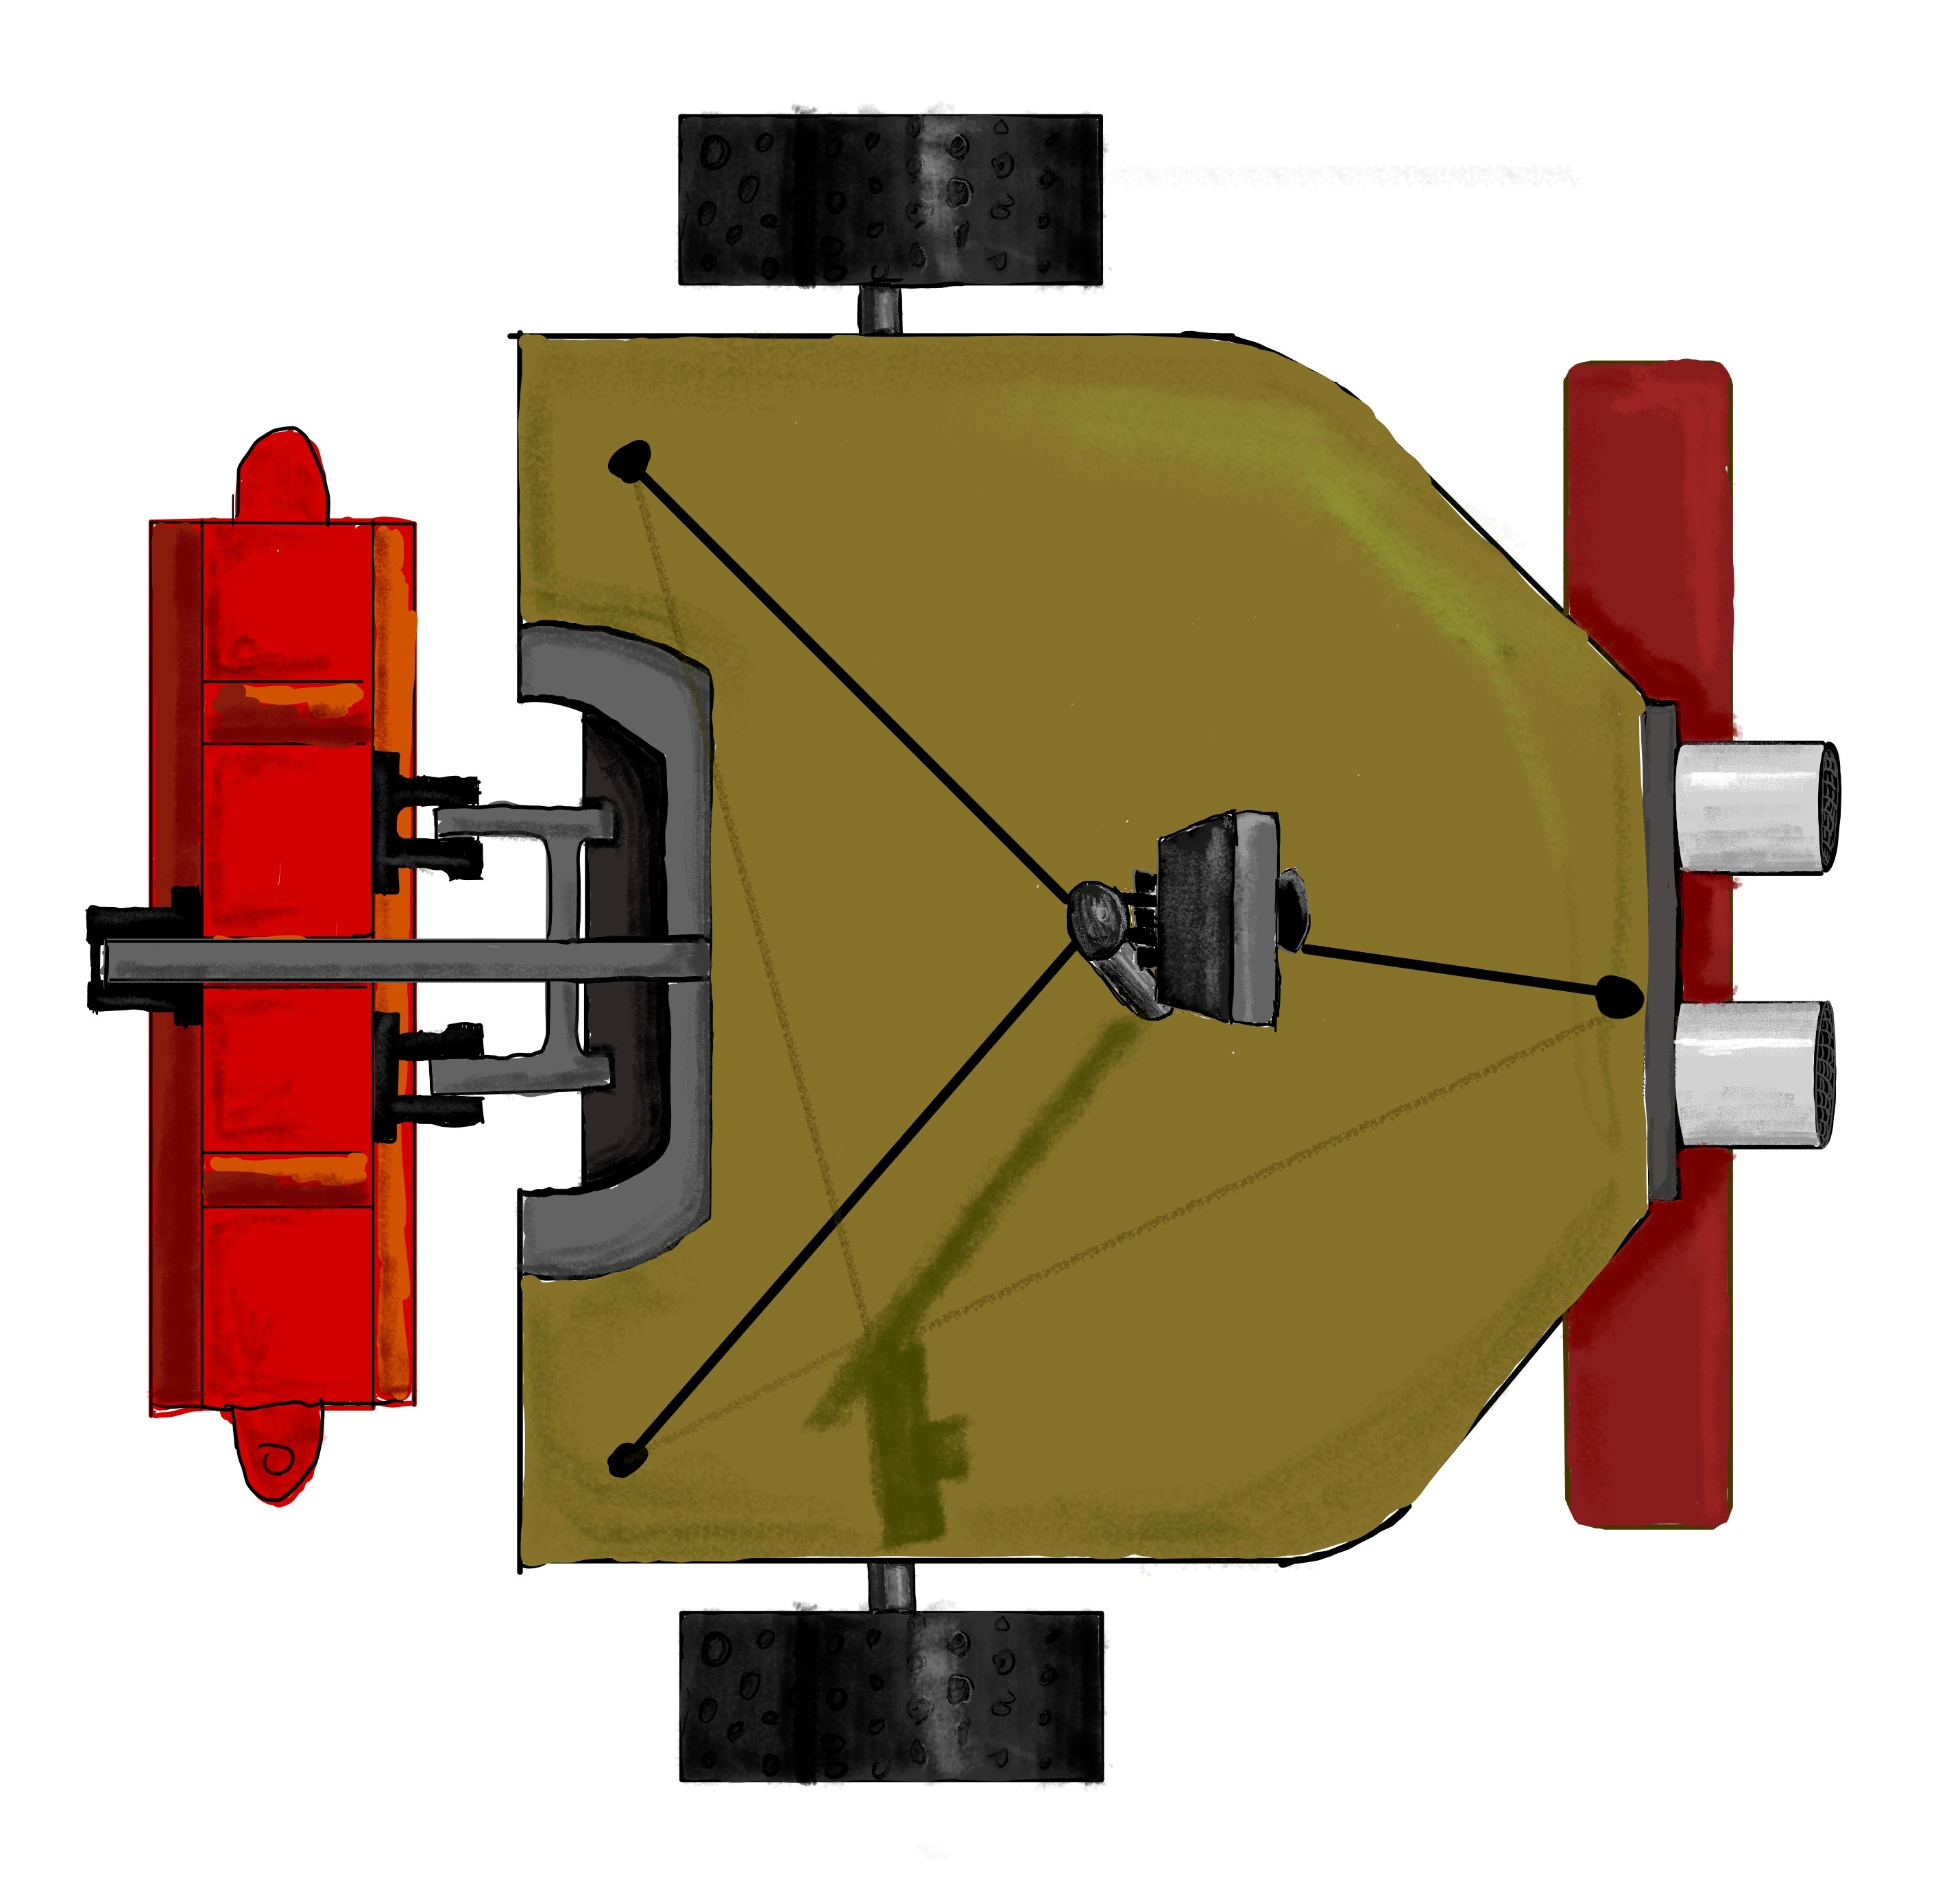
\includegraphics[width=0.5\textwidth]{assets/gesamtkonzept/Skizze-Fahrzeugkonzept.jpg}}


\author{
\begin{tabular}{ l l l}
  \textbf{Gruppe 4} && \\
    Schaffner Timo & timo.schaffner@stud.hslu.ch & Digital Engineering\\
  Kasper Jonah & jonah.kasper@stud.hslu.ch & Elektrotechnik\\
  Zimmermann Ivan & ivan.zimmermann@stud.hslu.ch & Elektrotechnik \\
  Schmid Lukas & lukas.schmid@stud.hslu.ch & Informatik\\
  Meyer Alina & alina.meyer@stud.hslu.ch & Informatik \\
  von Atzigen Elias & elias.vonatzigen@stud.hslu.ch & Maschinentechnik \\
  \\
  \textbf{Betreuender Dozent} && \\
  Thalmann Markus & markus.thalmann@hslu.ch & Elektrotechnik \\
  \\
  \\
  \\
  TA.BA\_PREN2.F2501 &&\\
\end{tabular}
}
\date{\today}


    \maketitle
    \newpage

    \section*{Abstract}

Abstract

Entweder hier: TODO PREN1 in ELEKTRONISCHER ANHANG

    \tableofcontents\thispagestyle{fancy}
    \newpage
    \listoffigures\thispagestyle{fancy}
    \newpage
    \listoftables
    \newpage
    \subfile{glossary.tex}

%%%%%%%%%%%%%%%%%%%%%%%%%%%%%%%%%%%%%%%%%%%%%%%%%%%%%%%%%%%%%%%%%%%%%%%%%%%%%%%%%%%%%%%%%%
%%%%%%%%%%%%%%%%%%%%%%%%%% Add your file here %%%%%%%%%%%%%%%%%%%%%%%%%%%%%%%%%%%%%%%%%%%%
%%%%%%%%%%%%%%%%%%%%%%%%%%%%%%%%%%%%%%%%%%%%%%%%%%%%%%%%%%%%%%%%%%%%%%%%%%%%%%%%%%%%%%%%%%

    % Include files
    \section{Einleitung}

In dieser Dokumentation wird die Umsetzung des im \acrfull{pren1} erarbeiteten Konzeptes beschrieben. 
Die Dokumentation, in der das Erarbeiten des Konzeptes detailliert ist, befindet sich im elektronischen Anhang und wird, wenn nötig im Text referenziert und alle Aenderungen werden hervorgehoben.

Der Roboter kann ein Wegenetzwerk traversieren und Hindernisse darauf erkennen und umgehen. Die genaue Aufgabenstellung inklusive der Anforderungsliste befinden sich im Anhang \nameref{aufgabenstellung} und \nameref{anforderungliste}. Das Projekt wird wieder in einem interdisziplinären Team durchgeführt. Das Team besteht aus Studierenden der Studiengänge \acrfull{maschinentechnik}, \acrfull{elektrotechnik}, \acrfull{informatik} und \acrfull{digitalengineering}. Alle für die Planung und Umsetzung benötigten Kompetenzen sind vorhanden.

In diesem Bericht werden zuerst die Risiken die während \acrshort{pren1} und \acrshort{pren2} indentifiziert wurden beschrieben. Bei allen Risiken, die mit Massnahmen beim Roboterbau stark mitigiert werden konnten, wird auf die Beschreibung der Mitigation referenziert. Danach wird der Roboterbau beschrieben. Dabei werden die einzelnen Teilfunktionen beschrieben und wie sie umgesetzt wurden. Es werden neben der Umsetzung auch alle Tests und zusätzliche Berechnung beschrieben, genau wie die Risikobewältigung. Ebenfalls wird das Gesamtkonzept aufgezeigt mit Verweisen zu den Teilfunktionen und den einzelnen Komponenten. Als nächstes Kapitel wird das gesamte Funktionsmuster anhand der Anforderungen bewertet. Vor dem Fazit wird auf die Nachhaltigkeit eingegangen. Als Schlussdiskussion werden das Gelernete, weitere Risiken und offene Punkte beschrieben. Im Anhang sind unter anderem die Projektplanung und die Kosten angehängt.


Das Ziel ist es, einen stabilen und funktionierenden Roboter zu haben. Dieser soll intensiv getestet sein und er sollte auf allfällige Risiken vorbereitet sein. Der Roboter wird zum Abschluss in Form eines Wettbewerbes gegen die anderen Roboter antreten. Das Ziel für dieses Team ist es, dass der Roboter erfolgreich das Wegenetzt traversieren kann und das Ziel erreicht. Der benötigte Zeitaufwand wird gegenüber einer stabilen Funktionalität nachrangig priorisiert.


    \section{Risikobewertung}


Die Risiken des Projektes sind in \acrshort{pren1} gesammelt und bewertet worden. Pro Risiko wurden Massnahmen zur Prävention und zur Mitigation gesammelt. Die Bewertung wurde durchgeführt vor dem Umsetzen der Massnahmen (V.) und nachher (N.). Dies ist in mehr Detail nachzulesen in der im Anhang angehängten Arbeit. Jedes Risiko hat in dieser Arbeit neu eine weitere Kolonne "Ref.". Diese zeigt auf, in welchem Kapitel beschrieben wird, wie das Risko behoben oder noch weiter mitigiert wurde, falls dies möglich war.

TODO: SOME IMG IN SOME WAY? Riskomatrix von PREN1 + neue Risiken

% Aus der Risikomatrix nach den Massnahmen geht hervor, dass die grössten Risiken, die beim Entwickeln des Roboters berücksichtigt werden müssen, die folgenden drei sind:

% \begin{itemize}
%     \item Risiko 2: Knoten werden nicht erkannt.
%     \item Risiko 7: Ein Objekt wird fehlerhaft gedeutet und falsche Wege werden intern entfernt.
%     \item Risiko 12: Der Roboter wählt einen falschen Pfad, weil die Hinderniserkennung fehlerhaft ist.
% \end{itemize}

Die folgende Tabelle \ref{table:risks} zeigt alle Risiken detailliert auf.

\begin{table}[H]
\centering
\small
\begin{tabularx}{\textwidth}{|c|X|X|X|c|c|c|}
\hline
  \textbf{Nr} & \textbf{Beschreibung} & \textbf{Prävention} & \textbf{Mitigation} & \textbf{V.} & \textbf{N.} & \textbf{Ref.}\\
  \hline
      1&Hindernisse werden nicht erkannt. &Mit vielen Bildern trainieren.& Distanzsensor erkennt Hindernisse, falls Bilderkennung nicht erkannt hat; Roboter fährt zurück, falls Distanzsensor erkennt.&20&5& \\
  \hline
2&Knoten werden nicht erkannt. &Viele Bilder in verschiedenen Situationen machen, um zu trainieren.&Linien werden erkannt und Roboter orientiert sich daran.&20& 12&\ref{model-results}\\
  \hline
      3&4 Minuten reichen nicht. &Testdurchfläufe in realistischen Umgebungen.&&8&4 &\ref{risks-sprint-2}\\
  \hline
      4& 1 Minute reicht nicht zum Aufbau.& Testdurchfläufe und einfaches Interface.&Zufälliges Ziel wird gewählt von SW, falls bei Start keines ausgewählt.&5&3 &\ref{zieleingabe}\\
  \hline
      5&Bodenfugen werden als Linie erkannt. & Testdurchfläufe in realistischen Umgebungen.&Kamera hilft Linien zu erkennen, hilft Roboter gerade zu stellen.&15&4& \\
  \hline
      6& Liniensensor fehlerhaft. &Sichere Implementation mit Tests.& Encoder Motoren.&8&3 &\\
  \hline
      7& Ein Objekt wird fälschlicherweise erkannt. &Knoten erkennen und nicht nur Hindernisse.&Roboter ist schnell genug, um Wege auszuprobieren und hat einen Trial \& Error Modus, der dies erlaubt.&16&6& \ref{model-results}\\
  \hline
      8&Hindernisse werden beim Anheben verschoben. &Robuste Greifmethode wählen und testen.&&12&8& \\
  \hline
      9&Überstrom bei blockierten Motoren. &Endschalter, Stromsensoren.&Abschalten bevor Bauteile beschädigt.&10&5& \\
  \hline
      10&Ungenaue Abfahrtsituation vom Knoten, Fahrzeug fährt von der Linie weg. &Liniensensor als Unterstützung, Kamera prüft Linie& Falls keine Linie mehr erkannt, rückwärts fahren und korrigieren.&15&5& \\
  \hline
      11&Die Kamera liefert unscharfe oder verzerrte unbrauchbare Bilder. &Verwendung von Kameras mit hoher Auflösung.&Falls Bilder unscharf sind, Roboter anhalten und neue Bilder aufnehmen.&12&6&\ref{risks-sprint-1} \\
  \hline
      12& Der Roboter wählt einen falschen Pfad, Objekte nicht erkann werden. &Optimierung der Hinderniserkennung.& Falls Fehlzustand auftritt, kann Roboter zu vorherigen Knoten fahren und das vorher Gelernte zurücksetzen. Roboter ist schnell.&12& 6&\ref{model-results}\\
  \hline

\end{tabularx}
\end{table}

\newpage

\begin{table}[H]
\centering
\small
\begin{tabularx}\textwidth{|c | X | X | X | c | c|c|}
\hline
  \textbf{Nr} & \textbf{Beschreibung} & \textbf{Prävention} & \textbf{Mitigation} & \textbf{V.} & \textbf{N.} & \textbf{Ref.}\\
  
  \hline
        13&Ein Softwarefehler führt zu einem Absturz während der Laufzeit, wodurch der Roboter stoppt oder Fehlfunktionen aufweist. &Exception Handling und umfangreiche Tests unter verschiedenen Bedingungen.&Automatischer SW-Neustart, Wiederaufnahme des letzten bekannten Zustands.&15&4&\ref{risks-sprint-2} \\
  \hline
      14&Ein Software-Update führt zu neuen Fehlern oder ist nicht kompatibel mit der aktuellen Hardware. &Gründliche Tests vor dem Rollout eines Updates.& Durch SW-Versionierung hat man die Möglichkeit, schnell zur vorherigen stabilen Version zurückzukehren.&6&2&\ref{navigation-arch} \\
  \hline
      15&Akkustand ist zu niedrig bei Start des Laufes. & Anzeige des Akkustandes. Leicht austauschbarer Akku. Akku aufladen.&Ein zweiter Akku, der voll aufgeladen ist.&5& 1&\\
  \hline
      16&Personenausfall durch Krankheit oder Unfall. &&Stellvertretungen und virtuelle Kommunikation.&6& 3&-\\
  \hline
      17&Datenkorruption. &&Regelmässige Backups. Alle Dokumente auf Teams erstellen. Dokumentation in LaTeX auf Overleaf. Durch Cronjob werden jeden Tag die .tex Files auf GitHub gepusht.&4& 1&-\\
  \hline
  \multicolumn{7}{l}{Neue Risiken aus PREN 2} \\
  \hline
  18&Akkuhalterung geht kaputt & Akku vorsichtig austauschen. & Mehrere Akkuhalterungen erstellen. & &&\\
  \hline
  19&Elektroteile geht kaputt & Vorsichtig damit umgehen und nicht unnötig anfassen. & Mehrere Exemplare bereithalten. & &&\ref{pcb}\\
  \hline
    20&Robtoter weiss nicht mehr wo er sich befindet.& Robuste Bilderkennung und Wegfindungsmethode. & Trial \& Error Modus implementieren. &&&\ref{navigation-arch}\\
  \hline
    21&Ausgehende Linien werden nicht erkannt. & Objekterkennung testen. & Aus anderer Distanz noch einmal versuchen und falls immer noch nicht erkannt, Knoten aus internem Graph entfernen. & &&\ref{outgoing-lines}\\
  \hline



\end{tabularx}
\caption{Risiken}
\label{table:risks}
\end{table}

TODO add those:

  - sprint 4 : gibt fälschlich an sei im Ziel obwohl nicht ist/ erkennt ziel nicht -> getestet mit X bildern und immer erkannt

TMP NOTES:

3: Risiko 1: ultraschall \\
3: Risiko 2: ok weil wenn ninchts erkannt einach Knoten \\
4: Risiko 3: schaffte immer in x min \\
4: Risiko 4: immer moeglich in x sec \\
Risiko 5:\\
Risiko 6:\\
3: Riisko 7: Model kann zu x prozent richtig, sonst wir gehofft dass nicht genug objekte gibt, dass alle wege wege sind, kamera winkel? Muss confidence level erreichen, damit nicht falsch deutet, lieber verpassen als erkennen wegen safety mit ultraschall\\
Risiko 8:\\
Risiko 9:\\
Risiko 10: durch tests: ist ok\\
1: Risiko 11: done\\
3: Risiko 12: Ultraschall erkennt \& setzt zurueck, faehrt zurueck\\
x: Risiko 13: in progress (link all times we mention unittests)\\
2: Risiko 14: done\\
Risiko 15:\\
16: -\\
17: -\\


    \section{Roboterbau}

In diesem Teil werden die einzelne Schritte beschrieben, um den Roboter zu bauen. Dabei wird sich an dem Konzept von \acrshort{pren1} orientiert. Falls von dem Konzept abgewichen wird, wird dies erwähnt und begründet. Die Arbeit aus \acrshort{pren1} kann im elektronischen Anhang gefunden werden.

Die folgenden Kapitel sind unterteilt nach den einzelnen Epics und User Stories, die im vorgehenden Kapitel \ref{projektplanung} aufgelistet wurden. Dabei werden die Tätigkeiten beschrieben, inklusive Testprotokolle und -beschriebe.

TODO: Risikoverweise (welches Risiko vermindert/behoben? Double checkwith table from prev chapter 
TODO: Testprotokolle
TODO: Lessons Learned
TODO: Komponentendiagramme mit Schnittstellen falls sinnvoll

TODO: 
Was vorkommen muss:
• Produktbeschreibung des Funktionsmusters (Hauptteil)
- Übersichtszeichnungen / Übersichtsmodell
- Beschreibung der Komponenten
- Ablaufdiagramme, Blockdiagramme
- Beschreibung der Funktionalität der einzelnen Blöcke und deren Beziehungen
- Schnittstellenbeschreibungen
- Softwaresubsysteme
- Wichtige Berechnungen (Resultate)
- Beschreibung von Versuchen und Tests mit Ergebnissen (Zusammenfassung)

\subsection{Produktbeschreibung}

In diesem Kapitel wird der Roboter als Gesamtsystem beschrieben. Dabei wird das Funktionsmuster mit einem Ablaufdiagramm beschrieben und die einzelnen physischen und elektronischen Komponenten werden in Zeichnungen aufgezeigt.


Die folgende Grafik \ref{fig:ablauf} zeigt das geplante Funktionsmuster auf. Dieses Ablaufdiagramm stammt aus \acrshort{pren1} und dient zur Erinnerung, genauere Informationen koennen aus der angehaengten PREN 1 Dokumentation entnommen werden.

\begin{figure}[H]
\centering
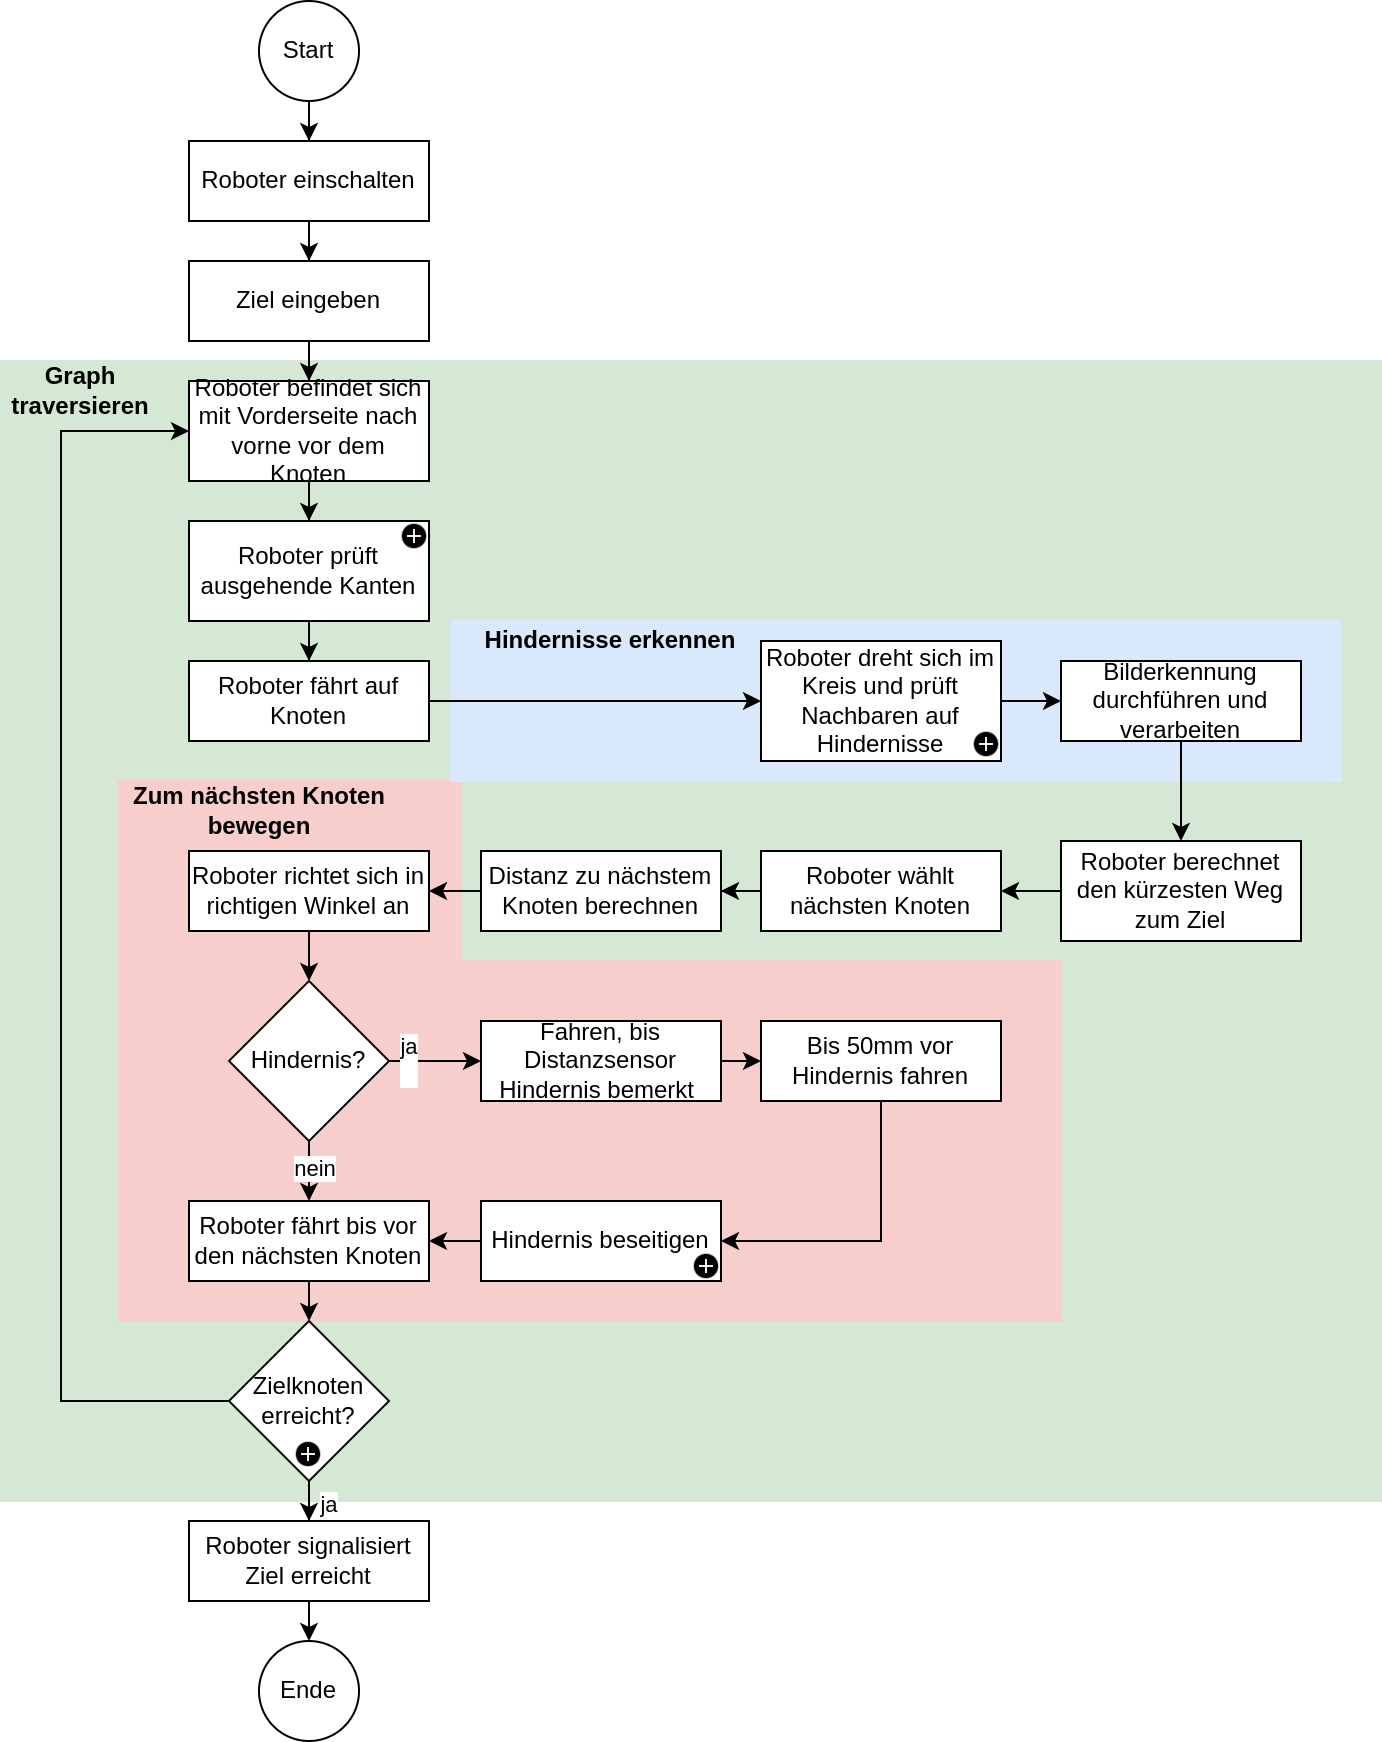
\includegraphics[width=\textwidth]{assets/gesamtkonzept/ablaufdiagramm.png}
\caption{Gesamtkonzept Ablaufdiagram}
\label{fig:ablauf}
\end{figure}

Damit dieses Funktionsmuster umgesetzt werden kann, wird ein Produkt mit folgenden Komponenten auf Grafik \ref{fig:components} gebaut. Die Grafik ist zeigt lediglich das Konzept mit den noetigen Komponenten und nicht das tatsaechliche Aussehen des Roboters.

\begin{figure}[H]
\centering
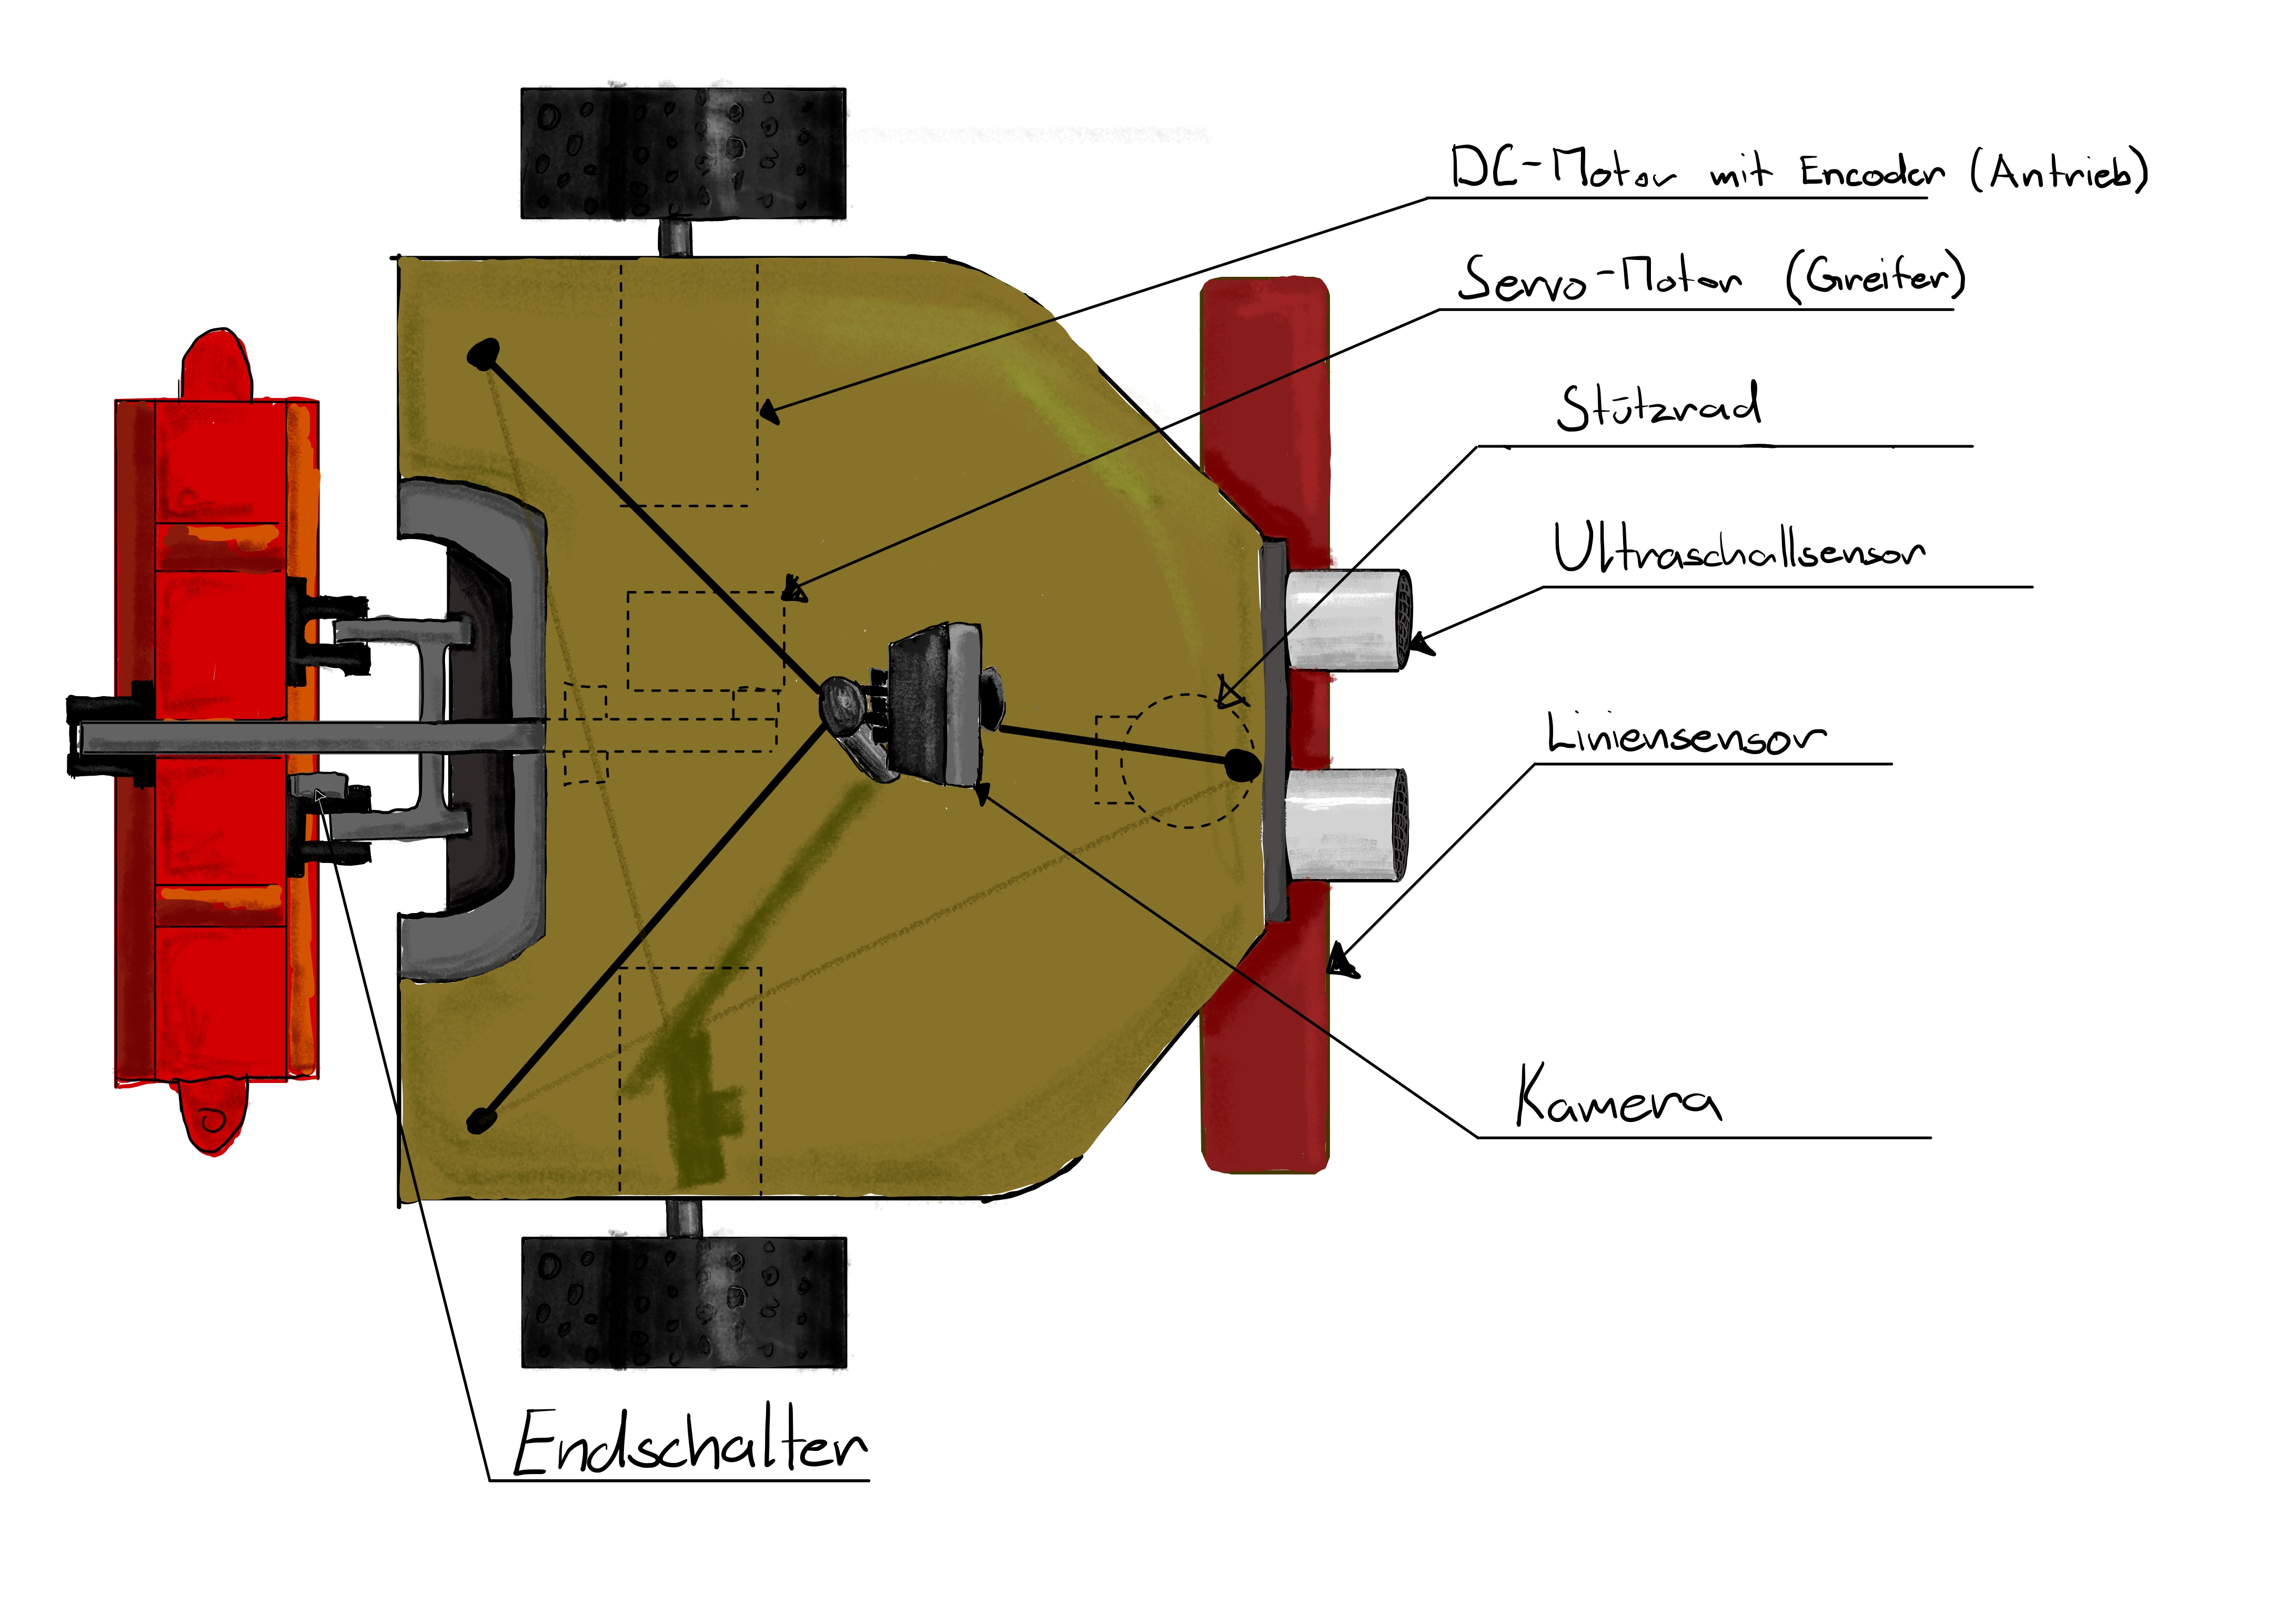
\includegraphics[width=\textwidth]{assets/gesamtkonzept/Skizze-Fahrzeugkonzept-Beschriftet.jpg}
\caption{Komponenten des Roboters}
\label{fig:components}
\end{figure}

Die einzelnen elektronischen Teile im Roboter bilden das Gesamtsystem ersichtlich auf Grafik \ref{fig:electro-components}. Dieses sorgt dafuer, dass sich der Roboter wie geplant autonom fortbewegen kann.

\begin{figure}[H]
\centering
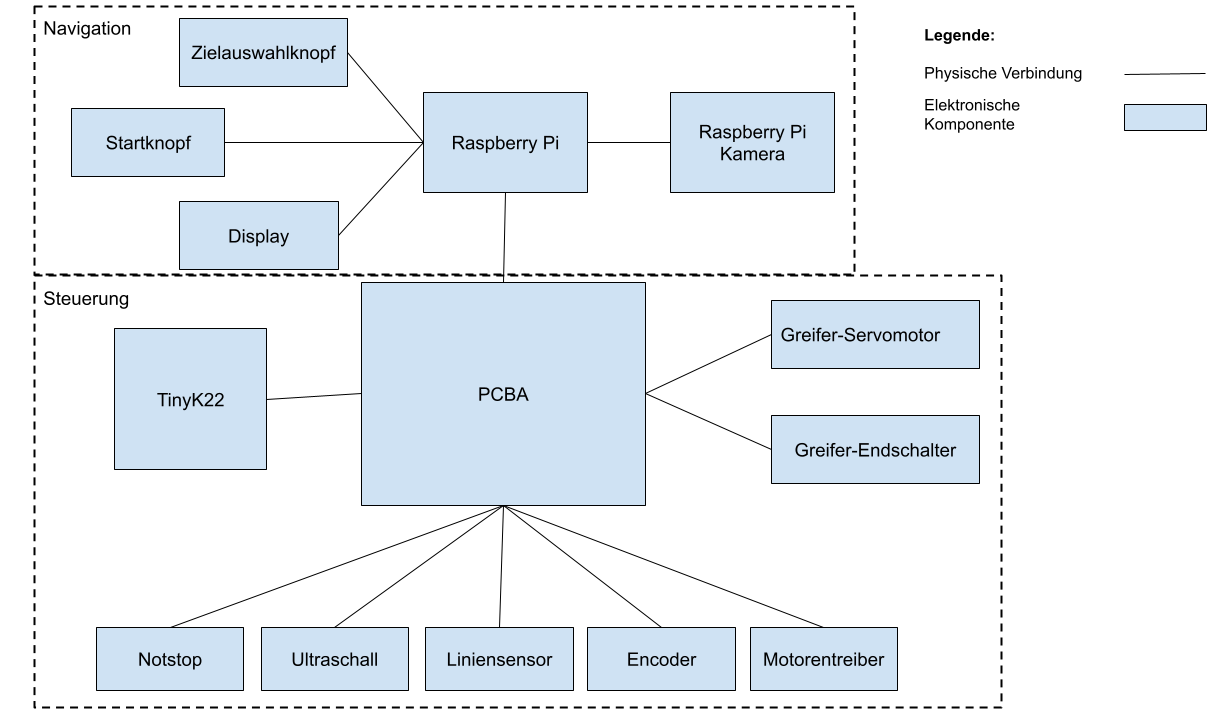
\includegraphics[width=\textwidth]{assets/gesamtkonzept/electronics.png}
\caption{Elektronische Komponenten des Roboters}
\label{fig:electro-components}
\end{figure} 

\newpage

%%%%%%%%%%%%%%%%%Epic 1%%%%%%%%%%%%%%%%%%%%%%%%%%%%%%%%%%%%%%%%%%%%%%%%%%%%%%%
\subsection{Fortbewegung mit geregelter Geschwindigkeit}

\subsubsection{Print Circuit Board design}
\label{pcb}

Um eine zuverlässige Kontaktierung der einzelnen Komponenten sicherzustellen, wird im Rah-
men von Pren 2 ein Verbindungs-PCB \ref{fig: Verteiler PCB} entwickelt. Dieses PCB übernimmt das Management der
Spannungsversorgung für den Raspberry Pi und den TinyK22. Zudem werden sämtliche Signale,
die vom TinyK22 erfasst und verarbeitet werden sollen, entsprechend verbunden.

\begin{figure}[H]
\centering
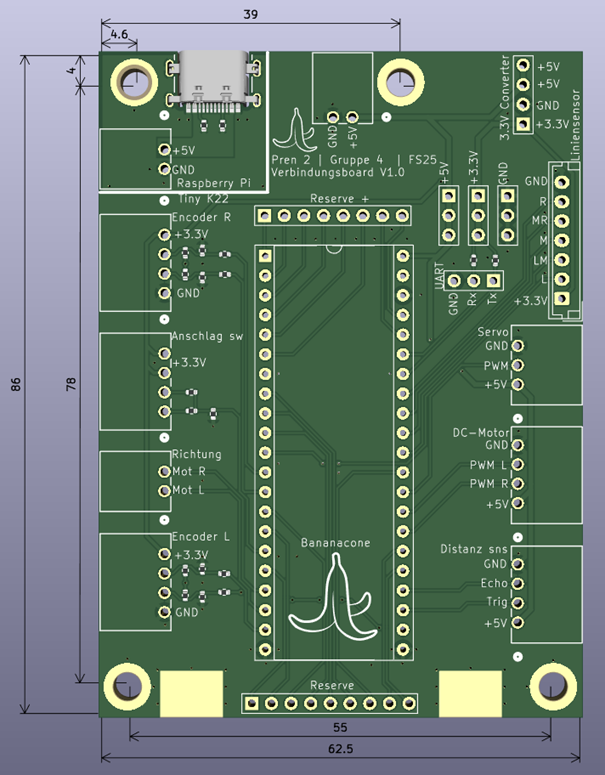
\includegraphics[width=5cm, height=6cm]{assets/ET/PCB/VerteilerPCB_unbestueckt.png}
\caption{Verteiler PCB}
\label{fig: Verteiler PCB}
\end{figure}

Von dem PCB wurden fünf Exemplare bestellt. Ebenso sind von dem TinyK22 mehrere Exemplare vorhanden \ref{fig: Verteiler PCBA}. Somit ist das Risiko der kaputten Elektroteile nicht mehr relevant.

\begin{figure}[H]
\centering
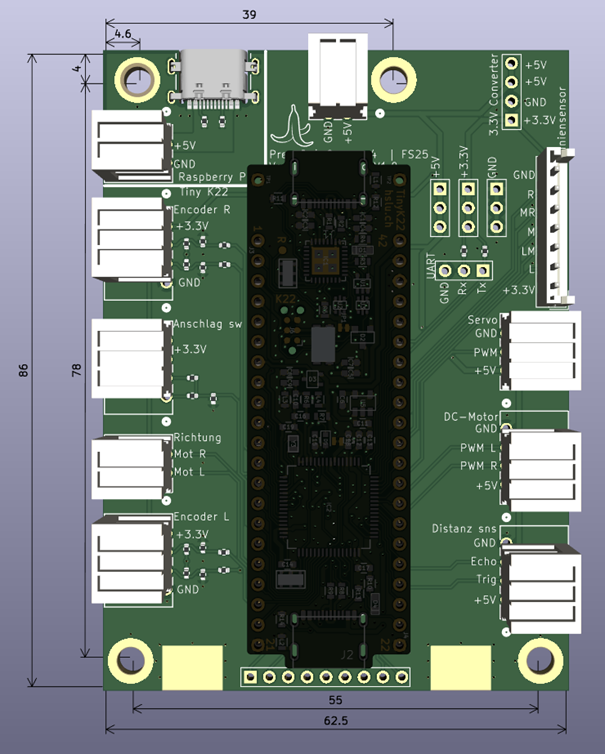
\includegraphics[width=5cm, height=6cm]{assets/ET/PCB/VerteilerPCB_bestueckt.png}
\caption{Verteiler PCBA}
\label{fig: Verteiler PCBA}
\end{figure}


\subsubsection{Motoren ansteueren und auslesen}

Nachdem die erste Ausführung der Software für die Motoren mit den beiden Encodern vorhanden war, wurde der implementierte Code mithilfe eines provisorischen Aufbaus getestet. Unter einem provisorischen Aufbau versteht man die Verwendung eines Breadboards mit dem TinyK22 und einem Speisegerät \ref{fig: Motorentest}. Allerdings wurde bereits der ausgewählte Motortreiber verwendet, der später auch im Endprodukt verbaut wird. Nach einigen Schwierigkeiten bei der Initialisierung des Quadratur-Encoder-Modus auf dem TinyK22 konnten die ersten Meter erfolgreich gefahren werden. Mit den ersten Erkenntnissen aus dem Test konnte die Software weiter angepasst werden, um immer präzisere Fahrmanöver auszuführen und die vorgegebenen Distanzen oder Drehwinkel exakt einzuhalten.


\begin{figure}[H]
\centering
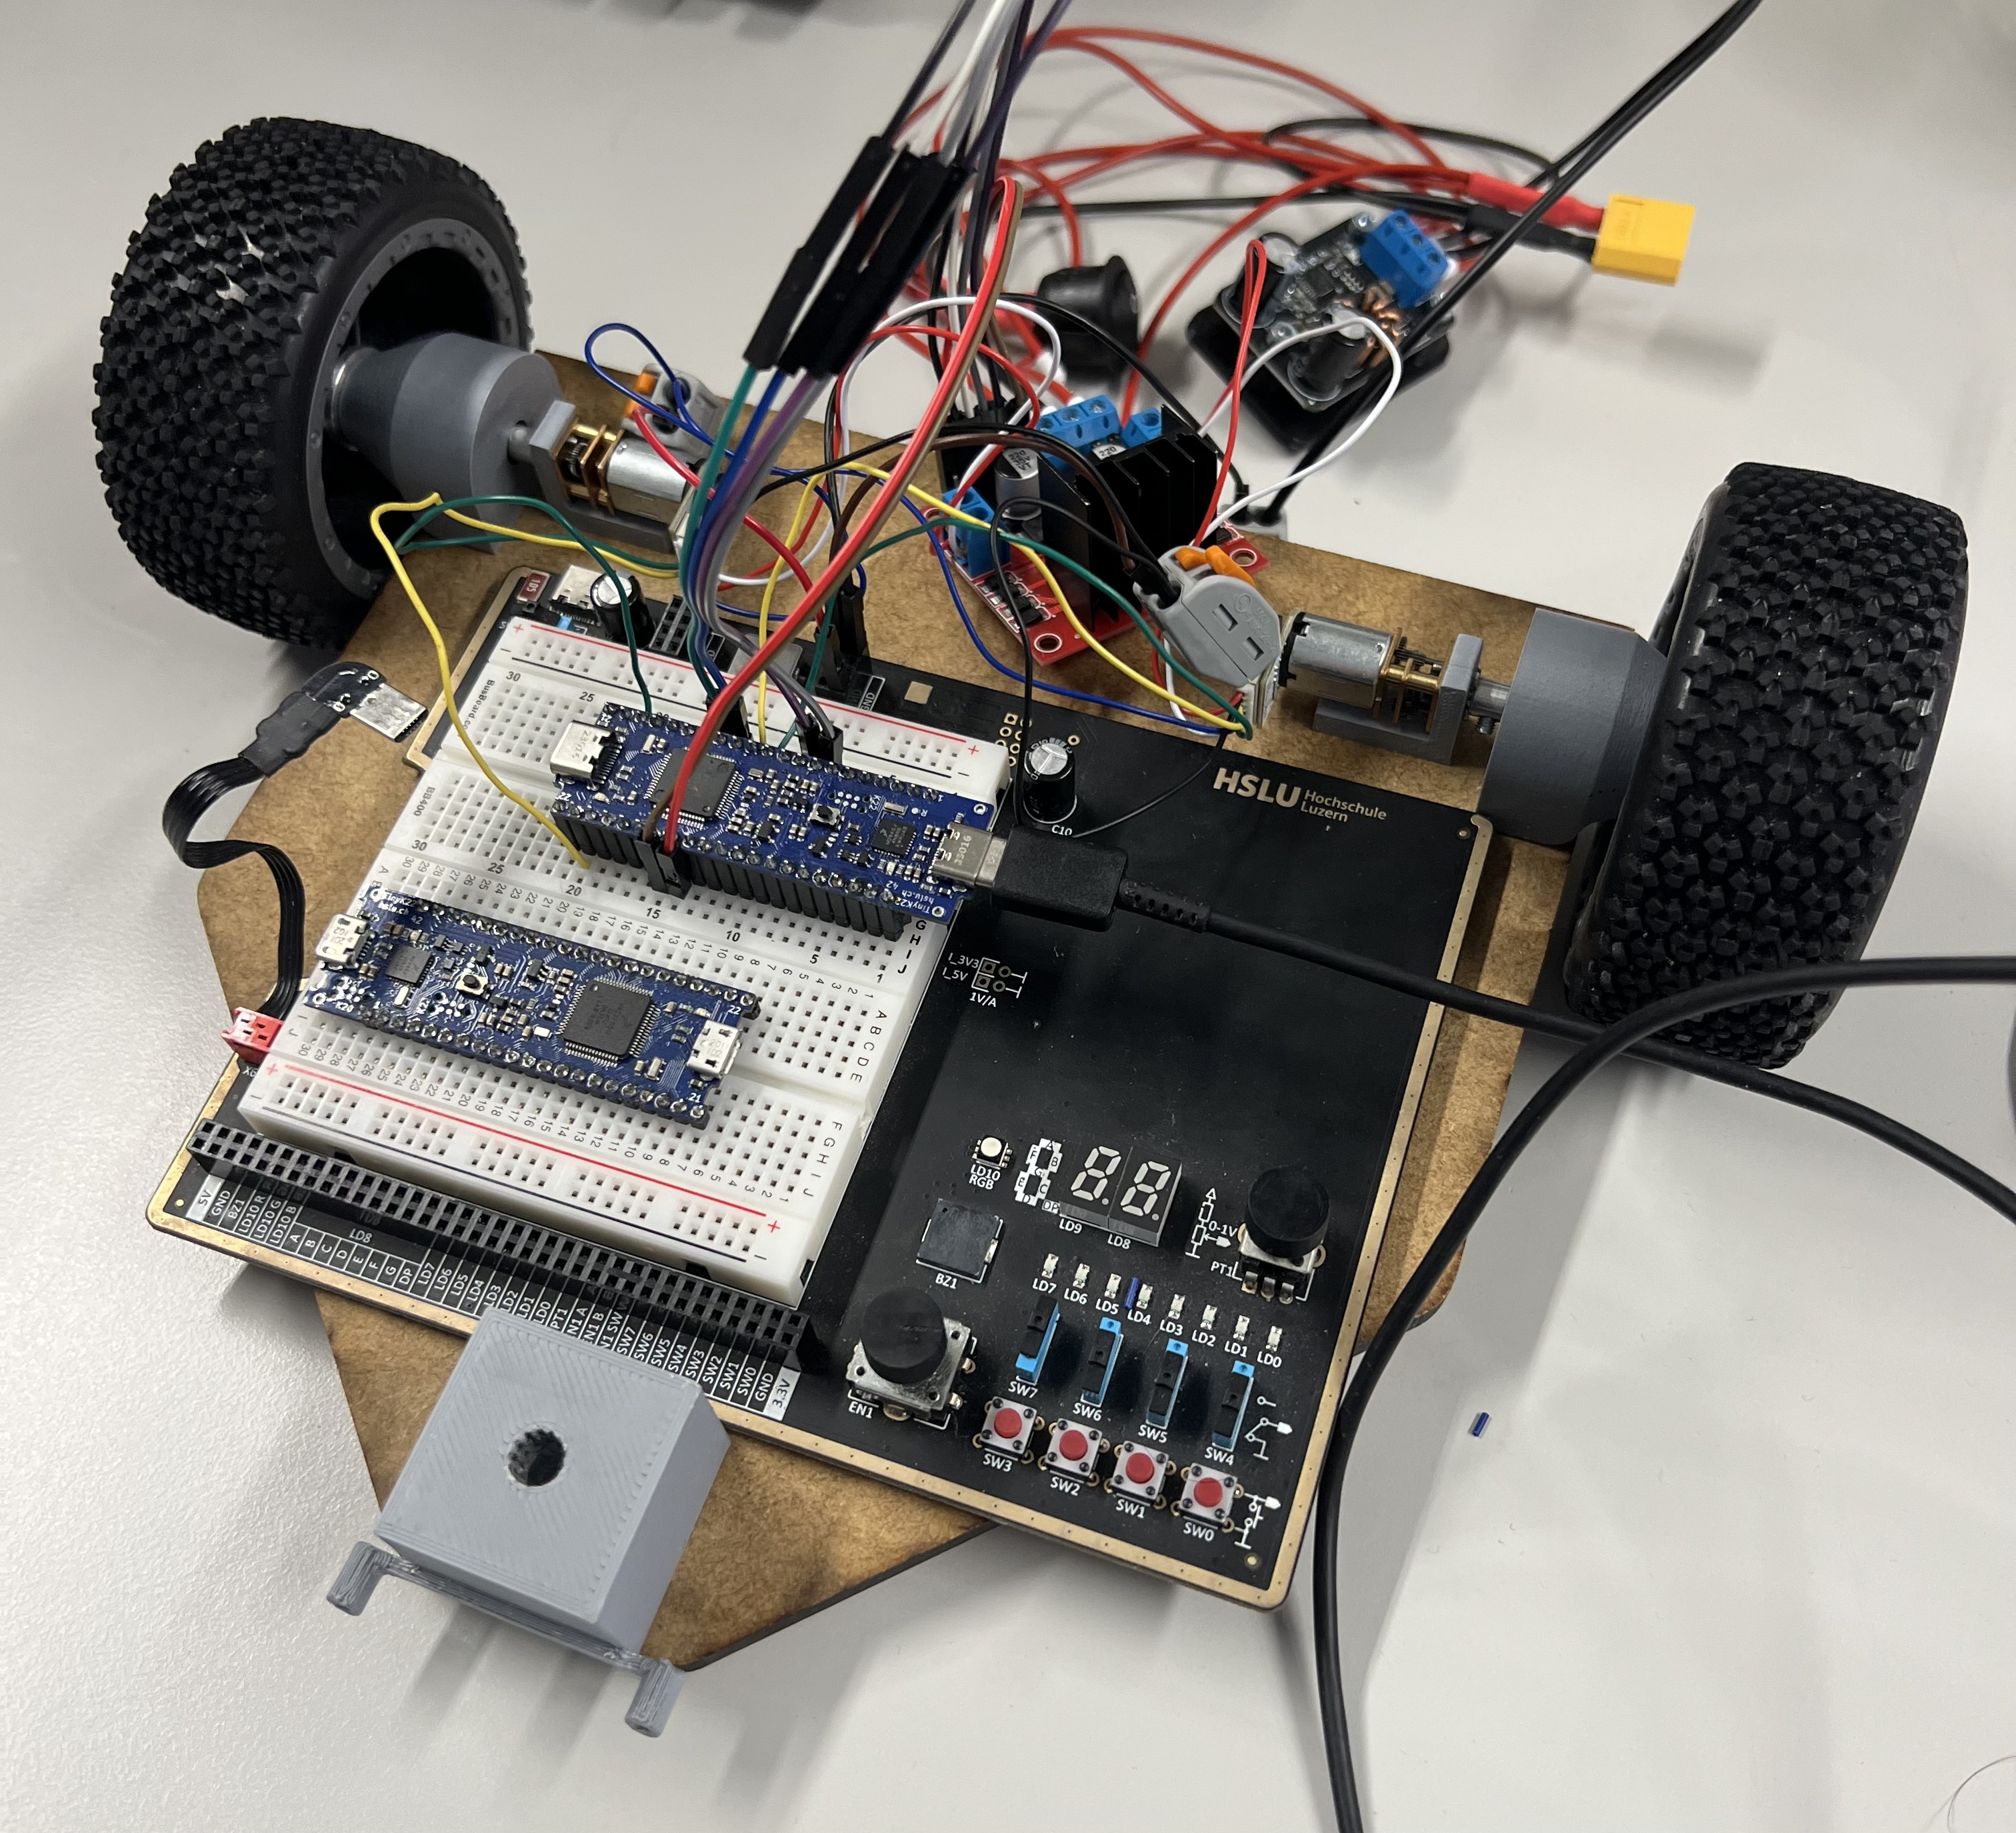
\includegraphics[width=10cm, height=8cm]{assets/ET/Motoren/Motorentest.jpeg}
\caption{Motorentest}
\label{fig: Motorentest}
\end{figure}

\subsubsection{Fahrwerk konstruieren}

 Das Konzept für das Fahrwerk und die Grundplatte wurden analog zum Konzept aus PREN1 umgesetzt. Am Fahrwerk wurden gegenüber des Prototyps aus PREN1 einzig der Motorflansch und der Lenkrollenhalter angepasst. Beim Prototyp in PREN1 hat sich gezeigt, dass eine reine Presspassung für die Befestigung der Lenkrolle im Lenkrollenhalter aus PLA nicht ausreichend ist. Aus diesem Grund wird die Lenkrolle jetzt mithilfe eines M4 Gewindestifts geklemmt. Abb.\ref{fig: Lenkrollenhalter V2} 

\begin{figure}[H]
\centering
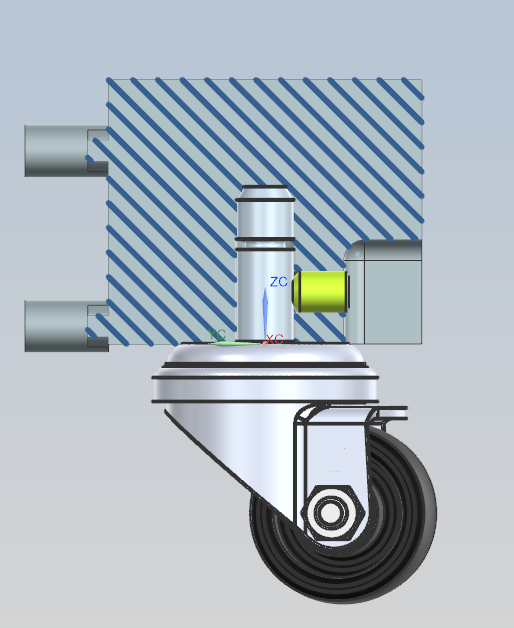
\includegraphics[width=5cm]{assets/MT/Lenkrollenhalter V2.png}
\caption{Lenkrollenhalter V2}
\label{fig: Lenkrollenhalter V2}
\end{figure}

Der Motorflansch wurde für den finalen Roboter leicht verstärkt. In  Abb. \ref{fig: Motorflansch V1/V2} sieht man in gelb die erste Version des Motorflansches wie er in PREN1 verbaut wurde. Blau eingefärbt die finale Version des Flansche mit einer Verstrebung. 

\begin{figure}[H]
\centering
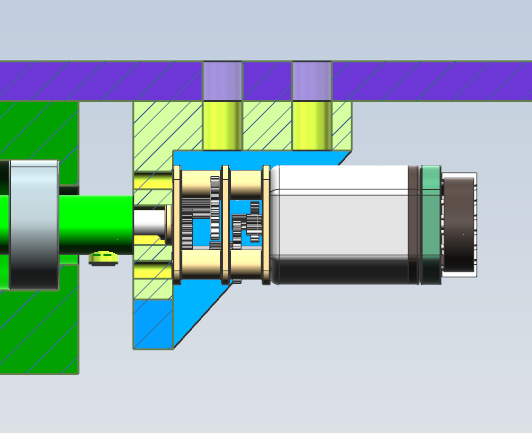
\includegraphics[width=5cm]{assets/MT/Motorflansch Vergleich.png}
\caption{Motorflansch V1/V2}
\label{fig: Motorflansch V1/V2}
\end{figure}

Die elektronischen Komponenten wie DC/DC-Konverter, Motortreiber oder RasberryPi werden nicht direkt auf die Grundplatte montiert, sondern auf Träger welche anschliessend auf die Grundplatte geschraubt werden. Die Träger wurden so konstruiert, dass die Kabel zwischen Träger und Bauteilen geführt werden können. (siehe Abb.\ref{fig: Träger für elektronische Komponenten}) Dieser Aufbau hatte in der frühen Testphase den Vorteil das alle elektronischen Komponenten provisorisch platziert werden konnten ohne einen Kurzschluss zu Riskieren. 

\begin{figure}[H]
\centering
\includegraphics[width=5cm]{assets/MT/Träger El Komponenten.jpg}
\caption{Träger für elektronische Komponenten werden zur Kabelführung verwendet}
\label{fig: Träger für elektronische Komponenten}
\end{figure}


Der Klemm- und Hebemechanismus des Greifers sind Abhängig von der Federkraft und den Lagerstellen. Bei der Implementierung des Greifers musste darauf geachtet werden das die Lagerstellen nicht verschoben werden. In Abb \ref{fig:Greifer im Roboter} \& \ref{fig:Greifer Versuchsaufbau} sieht man, die für die Funktion wichtigsten Masse am Versuchsaufbau und am Fertigen Roboter. Die für für die Haltekraft verantwortliche Feder, sowie alle Haltebacken und Pendelstützen wurden vom Prototyp wiederverwendet. 

\begin{figure}[H]
  \centering
  \begin{minipage}[b]{0.45\textwidth}
    \centering
    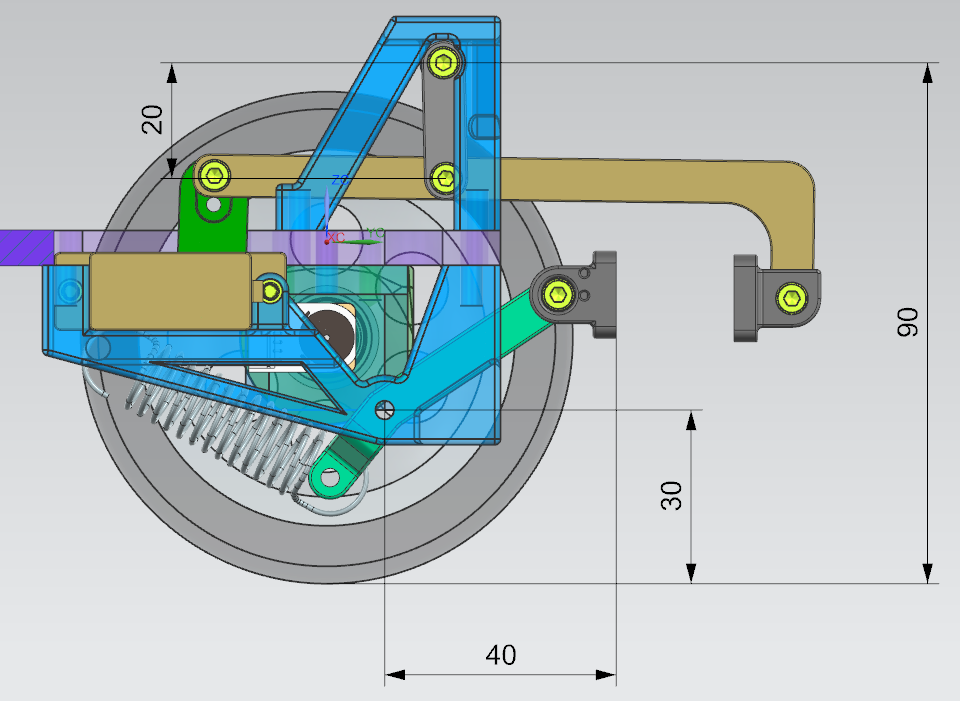
\includegraphics[height=5cm]{assets/MT/Greifer Montiert.png}
    \caption{Greifer im Roboter}
    \label{fig:Greifer im Roboter}
  \end{minipage}
  \hfill
  \begin{minipage}[b]{0.45\textwidth}
    \centering
    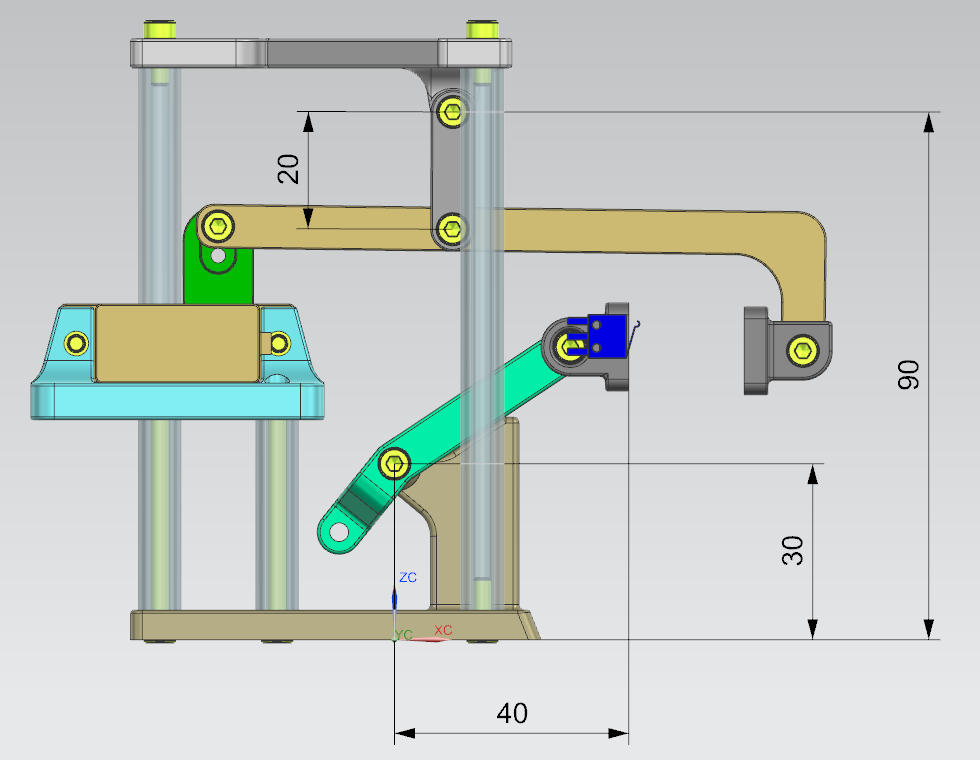
\includegraphics[height=5cm]{assets/MT/Greifer Prototyp.png}
    \caption{Greifer Versuchsaufbau}
    \label{fig:Greifer Versuchsaufbau}
  \end{minipage}
\end{figure}

exakte Position der Kamera und den Anstellwinkel 

-Raeder, PCB, Tiny, Akku, Motoren


\newpage
%%%%%%%%%%%%%%%%%Epic 2%%%%%%%%%%%%%%%%%%%%%%%%%%%%%%%%%%%%%%%%%%%%%%%%%%%%%%%

\subsection{Auf Linien des Graphes bewegen}

\subsubsection{Liniensensor auslesen}

In einem ersten Durchlauf wurde ein Code implementiert, um die Funktion mit dem TinyK22 zu testen. Mittels eines Timers wurden die einzelnen Pins in einem genügend grossen Zeitabstand von Vcc auf Input Capture umgeschaltet. Nach dem Umschalten auf Input Capture sollten sich die Kondensatoren je nach Reflexion des Untergrunds in unterschiedlichen Zeiten entladen. Dieses Verhalten konnte im Testprogramm dann auch erfolgreich festgestellt werden, durch die unterschiedlichen Werten im Timer Register des Input Capture Modus.


TODO: schönes Bild vom Testgestell mit/für Liniensnesor

\subsubsection{Liniensensor mit Abschirmung anbringen}

Nach dem ersten Test wurde der Liniensensor am Fahrzeug angebracht. Um Störeinflüsse von aussen zu vermeiden, wurde eine Abdeckung konstruiert, die jegliche Einstrahlung abschirmt. Dank diesem Aufbau konnte mit der weiteren Implementierung begonnen werden. Für die Feineinstellung wurden die einzelnen Sensorwerte auf dem Originalboden ausgemessen – ebenso auf dem Klebeband, da dies essenziell ist, um die Regelung sauber abzustimmen.



TODO: schönes Bild vom Schlussgestell mit Abschirmung des Liniensensors


\newpage
%%%%%%%%%%%%%%%%%Epic 3%%%%%%%%%%%%%%%%%%%%%%%%%%%%%%%%%%%%%%%%%%%%%%%%%%%%%%%

\subsection{Bis zum nächsten Knoten fahren}

\subsubsection{Kameranbindung}

...

\subsubsection{Distanz berechnen}

... POSSIBLY REMOVE TODO



... POSSIBLY REMOVE TODO

\subsubsection{Liniensensor}

Die Liniensensoren wurden wie geplant implementiert. Durch das Ummuxxen der Pins von GPIO-Output (High) auf den Input-Capture-Modus wird die Entladezeit eines Kondensators gemessen. Diese Zeit (ausgedrückt in Ticks) liefert Informationen darüber, ob sich das Fahrzeug über dem Soll-Fahrtweg befindet oder davon abweicht. Während der Fahrt werden die Sensor-Pins periodisch zwischen GPIO High und Input Capture umgeschaltet, um kontinuierlich neue Messwerte zu erhalten. Die erfassten Ticks werden in einer PD-Regelung weiter verarbeitet, welche die Abweichung zur Soll-Position (Linie) berechnet und entsprechend die Motoren nachsteuert. Diese Regelung ergänzt die Wegmessung über die Encodersensoren und erhöht die Spurtreue, indem sie sicherstellt, dass das Fahrzeug die Linie nicht verlässt.
    %%%%%%%%%%%%%%%%%Epic 4%%%%%%%%%%%%%%%%%%%%%%%%%%%%%%%%%%%%%%%%%%%%%%%%%%%%%%%
\subsection{Wegfindung}

In diesem Kapitel wird die Umsetzung der Wegfindung beschrieben. Ziel davon ist es, dass aufgrund von einem konfigurierten Graphen der schnellste Weg gefunden werden kann und die Kommunikation zwischen Navigation und Steuerung durchgeführt werden kann.

Das Finden des schnellsten Weg in einem Graphen wurde bereits in PREN 1 im Simulator umgesetzt mit einem Dijkstra Algorithmus. Der Simulator wird refactored, damit möglichst viele Teile wiederverwendet werden können.

\subsubsection{Wegfindungssoftware aus Simulator anpassen}
\label{navigation-arch}

Bevor der Simulator refactored wurde, wurde die neue Architektur designed für die Navigation, die auf Grafik \ref{fig:nav-arch} sichtbar ist.

\begin{figure}[H]
\centering
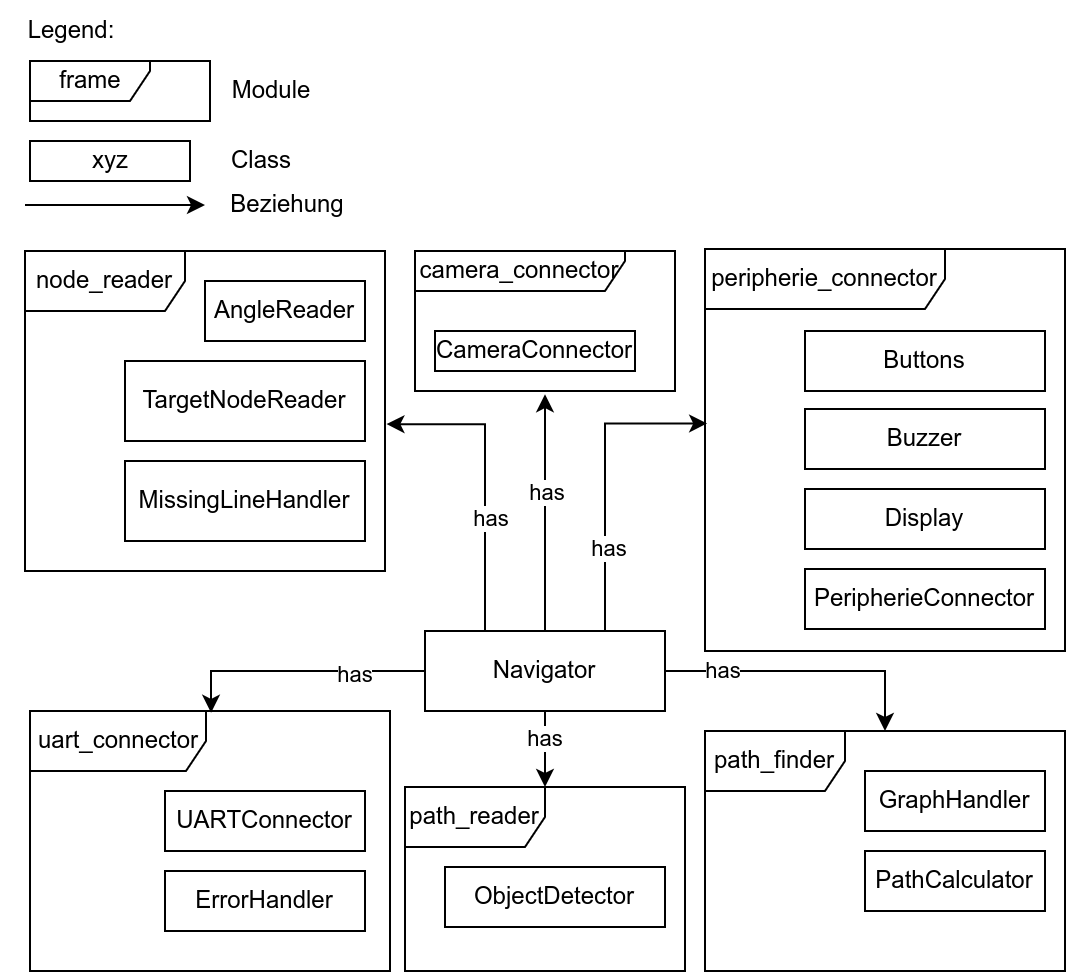
\includegraphics[width=\textwidth]{assets/IT/robot-sw-architecture-arch.png}
\caption{Aufbau Interface zu Steuerung}
\label{fig:nav-arch}
\end{figure}

Dieses Refactoring hilft dabei, dass strukturiert die simulierten Teile mit den realen Teilen ersetzt werden können und währenddessen sowohl auf einem Raspberry Pi, mit allen Verbindungen, als auch auf einem Laptop mit keinen Verbindungen eine lauffähige Version des Simulators verfügbar ist.
Durch verschiedene Environment Variablen\footnote{\url{https://de.wikipedia.org/wiki/Umgebungsvariable}} können die Hardware und der Funktionsumfang dynamisch gewählt werden. Nachfolgend in Tabelle \ref{table:environment-variables} sind diese Variablen ersichtlich


\begin{table}[H]
    \centering
    \begin{tabularx}{\textwidth}{|X|X|X|}
    \hline
        \textbf{Environment Variable} & \textbf{Beschreibung} & \textbf{Mögliche Werte}\\
        \hline
         \verb|PREN_PLATFORM| & Die Platform, auf welchem der Code ausgeführt wird. & \verb|PC| oder \verb|RPI| \\
         \hline
         \verb|PREN_CAMERA| & Die verwendete Kamera & \verb|NONE|, \verb|USB| oder \verb|PICAMERA| \\
         \hline
         \verb|PREN_UART| & Die verwendete Serielle Schnittstelle für die Kommunikation zwischen Raspberry Pi und \gls{tinyk22} & \verb|NONE| oder \verb|<DEVICE>| \newline (z.B. \verb|/dev/ttyAMA0|) \\
         \hline
         \verb|PREN_DISPLAY| & Das verwendete Display &  \verb|NONE|, \verb|OLED| oder \verb|TERMINAL|  \\
         \hline
    \end{tabularx}
    \caption{Environment Variabeln}
    \label{table:environment-variables}
\end{table}

Bei jedem Update wird getestet, ob die Version noch auf allen Plattformen lauffähig ist. Falls dies nicht der Fall wäre, kann durch die Benutzung von Git einfach auf eine alte Version zurück gewechselt werden. So muss das Risiko 14 von Software Updates, die Fehler mit sich bringen, nicht mehr beachtet werden.

Sowohl der Ablauf aus der Navigation selber die Berechnung der kürzesten Pfades und die interne Behandlung des Graphen sind gleicht wie in \acrshort{pren1} und sind auf den folgenden Grafiken \ref{fig:nav-navigator} und \ref{fig:nav-pathfinder} als Wiederholung gezeigt. Der Rest der einzelnen Module wird in den folgenden Kapiteln Schritt für Schritt im Detail aufgezeigt.

\begin{figure}[H]
  \centering
    \begin{minipage}[b]{0.48\textwidth}
    \centering
    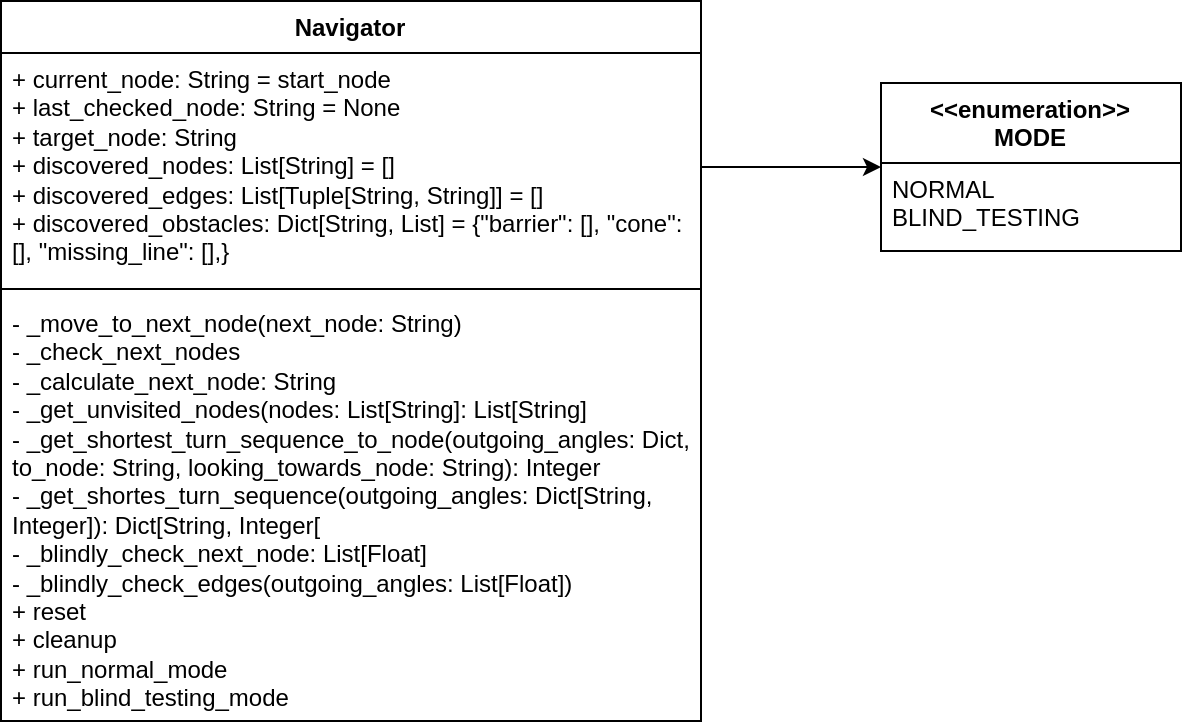
\includegraphics[width=\textwidth]{assets/IT/robot-sw-architecture-navigator.png}
    \caption{Navigator Modul}
    \label{fig:nav-navigator}
  \end{minipage}
  \hfill
  \begin{minipage}[b]{0.48\textwidth}
    \centering
    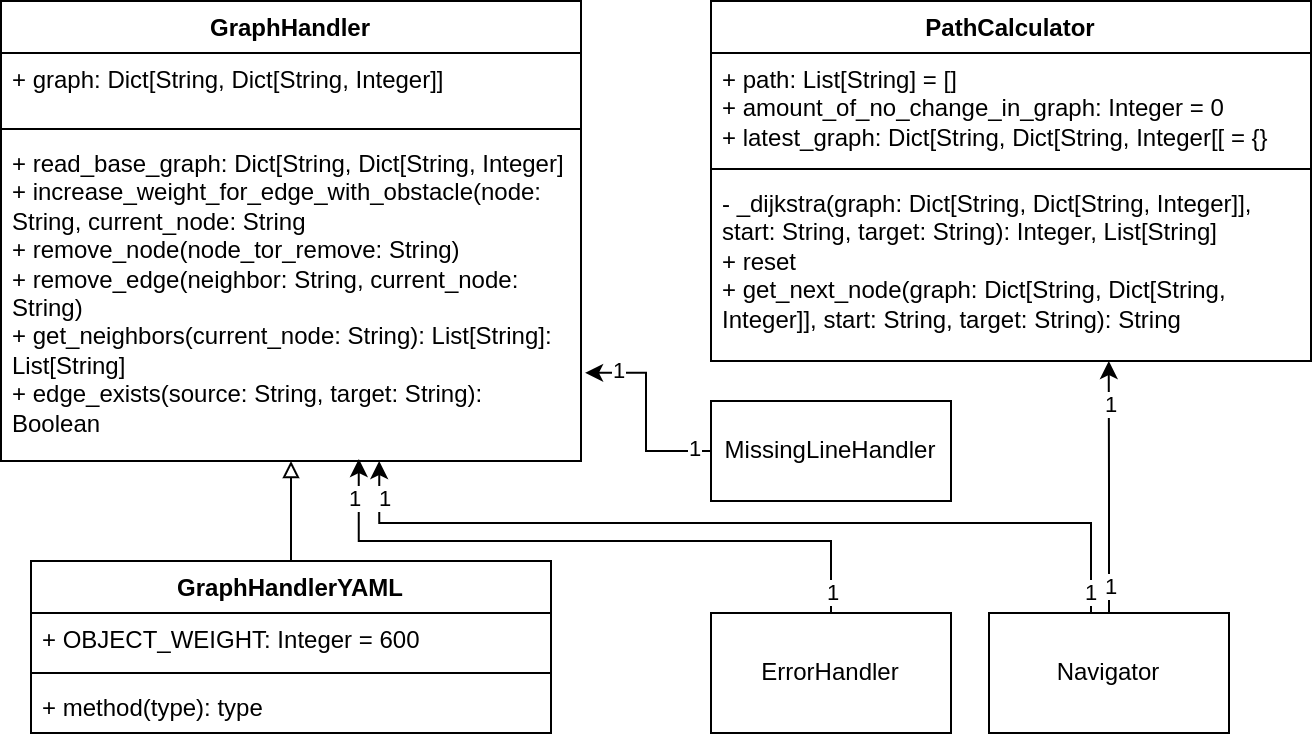
\includegraphics[width=\textwidth]{assets/IT/robot-sw-architecture-path_finder.png}
    \caption{Path Finder Modul}
    \label{fig:nav-pathfinder}
  \end{minipage}
\end{figure}

Ein grosser Unterschied von der neuen Architektur zu der Architektur des Simulators ist es, dass es eine klare Unterteilung in die einzelnen Module gibt, die die Navigation benötigt. So wird paralleles Arbeiten einfacher. Die Architektur modelliert nicht mehr die physischen Roboterteile, sondern nur noch die Navigationsteile.

Der gesamte Sourcecode zu der Navigation kann im Github-Repository (\url{https://github.com/ameyer3/hslu-pren-navigation}) oder im elektronischen Anhang gefunden werden.

Wie im Simulator aus \acrshort{pren1}, wird in der Navigation ein Trial \& Error Modus implementiert. Dieser Modus wird Blind Testing Mode genannt und wird eingeschaltet, falls es wirkt, als ob der Roboter nicht mehr weiss wo er sich befindet, beziehungsweise, falls er denkt er befindet sich auf einem anderen Knoten als er es tatsächlich tut. Die folgenden Situationen sind Zeichen, dass dies der Fall ist:

\begin{itemize}
    \item Roboter detektiert mehr ausgehenden Kanten von einem Knoten als erwartet.
    \item Falls in einem Winkelbereich, indem keine oder eine Kante erkannt werden soll, zwei Kanten erkannt werden.
    \item Falls der Dijkstra Algorithmus keine Route zum Ziel mehr findet.
\end{itemize}

Im Blind Testing Mode nimmt der Roboter jedes Mal die erste Kante von links, bei der keine Pylone erkannt wird und sucht so das Ziel. Obwohl es möglich ist, dass falsche Kanten entfernt werden und dies nicht auffällt, wird dies akzeptiert. Falls immer noch ein Weg gefunden kann, wird dieser zwar länger dauern, dies wird aber in Kauf genommen. Mit diesem Konzept können Risiko 20 (Roboter weiss nicht mehr wo er sich befindet) und Risiko 7 (Hindernis wird fälschlicherweise erkannt) so stark mitigiert werden, dass sie vernachlässigt werden können.

\subsubsection{Schnittstelle Navigation und Steuerung}
\label{interface-nav-control}

Die Navigation läuft auf einem Raspberry Pi und die Steuerung läuft auf einem \gls{tinyk22}. Die beiden kommunizieren wie geplant über das UART Protokoll miteinander. Für die Kommunikation wurde eine Schnittstelle definiert. Die Navigation sendet 4 Bytes an die Steuerung und die Steuerung antwortet mit dem Statuscode in Form von einem Byte.

Die Instruktionen von der Navigation an die Steuerung, werden, wie in Grafik \ref{fig:interface-tiny} gezeigt, gesendet.

\begin{figure}[H]
\centering
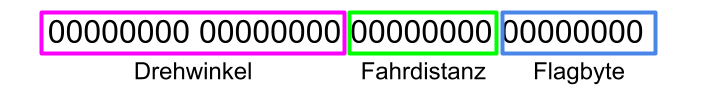
\includegraphics[width=\textwidth]{assets/IT/interface-tiny.png}
\caption{Aufbau Interface zu Steuerung}
\label{fig:interface-tiny}
\end{figure}

Die einzelnen Bytes sind in der folgenden Tabelle \ref{table:interface-to-tiny} beschrieben.

\begin{table}[H]
\centering
\small
\begin{tabularx}{\textwidth}{|c|c|X|}
\hline
  \textbf{Byte} &\textbf{Bezeichnung} & \textbf{Beschreibung}\\
  \hline
      1. Byte&1. Winkelbyte &Zeigt zusammen mit dem 2. Winkelbyte den Drehwinkel an. Die Steuerung addiert die beiden Werte und gibt den Befehl, dass der Roboter sich so weit drehen soll. In zwei Bytes aufgeteilt, da der Drehwinkel 255 übersteigen kann.\\
  \hline
2. Byte&2. Winkelbyte&Siehe 1. Winkelbyte.\\
  \hline
  3. Byte&Fahrbyte&Gibt die Distanz in Zentimeter an, die der Roboter fahren soll.\\
  \hline
  4. Byte&Flagbyte&Gibt an, ob der Roboter sich nach links oder rechts drehen soll, ob der Roboter vorwärts oder rückwärts fahren soll, ob sich eine Barriere auf der folgenden Strecke befindet.\\
  \hline
  \end{tabularx}
\caption{Interface zu Steurung}
\label{table:interface-to-tiny}
\end{table}

Die einzelnen Bedeutungen zu den Möglichkeiten des Flagbytes sind in Tabelle \ref{table:flag-to-tiny} erklärt.

\begin{table}[H]
\centering
\small
\begin{tabularx}{\textwidth}{|c|X|X|}
\hline
  \textbf{Flagbyte} & \textbf{Bedingung} & \textbf{Beschreibung}\\
  \hline
      0000&nur Winkelbyte gesetzt&Roboter soll sich nach links drehen.\\
  \hline
        0000&nur Fahrbyte gesetzt&Roboter soll vorwärts fahren.\\
  \hline
0001&nur Winkelbyte gesetzt&Roboter soll sich nach rechts drehen.\\
  \hline

0010&nur Fahrbyte gesetzt&Roboter soll rückwärts fahren.\\
  \hline

0100&kein zusätzliches Byte gesetzt&Auf folgender Strecke befindet sich eine Barriere.\\
  \hline
1000&kein zusätzliches Byte gesetzt&Roboter fährt bis er sich auf einem Knoten befindet.\\
  \hline
  \end{tabularx}
\caption{Flags in Interface zu Steurung}
\label{table:flag-to-tiny}
\end{table}



Die möglichen Statuscodes von der Steuerung an der Navigation sind in folgender Tabelle \ref{table:statuscodes} aufgelistet.

\begin{table}[H]
\centering
\small
\begin{tabularx}{\textwidth}{|c|l|X|}
\hline
  \textbf{Statusbyte} & \textbf{Encoding} & \textbf{Beschreibung} \\
  \hline
      00000000&SUCCESSFULLY\_DONE&Befehl wurde erfolgreich ausgeführt. \\
  \hline
00000001&UNEXPECTED\_OBJECT\_DETECTED &Ultraschall hat ein Objekt erkannt, das nicht erwartet wurde. Navigation macht ein Bild und detektiert, um welches Objekt es sich handelt und handelt entsprechend (mitigiert Risiko 12 (übersehene Objekte)): Kehrt um, falls Pylone oder beseitigt, falls Barriere.\\
  \hline
\end{tabularx}
\caption{Statuscodes von Steuerung}
\label{table:statuscodes}
\end{table}

\textbf{\gls{tinyk22} Implementation}

Für jedes empfangene Byte wird auf dem \gls{tinyk22} ein Interrupt generiert und anschliessend ausgelesen. Das Byte wird in einem Buffer Array zwischengespeichert. Nachdem die festgelegten 4 Bytes angekommen sind werden, die im Buffer zwischengespeicherten Bytes, in ein Array geschrieben. Aus diesem Array können dann die einzelnen Funktionen die nötigen Daten entnehmen und weiter verwenden.

\textbf{Raspberry Pi Implementation}

Auf dem Raspberry Pi wurde UART aktiviert, damit dieser mit dem \gls{tinyk22} kommunizieren kann.
Für die Kommunikation wird ein uart\_connector Modul erstellt. Dieses besteht aus der UARTConnector Klasse und der ErrorHandler Klasse, die die statische Methode 'handle\_errors' enthält. Auf folgender Grafik \ref{fig:uart-connector-nav} sind die beiden Klassen im Detail dargestellt mit ihrer Beziehung zu den anderen Klassen.

\begin{figure}[H]
\centering
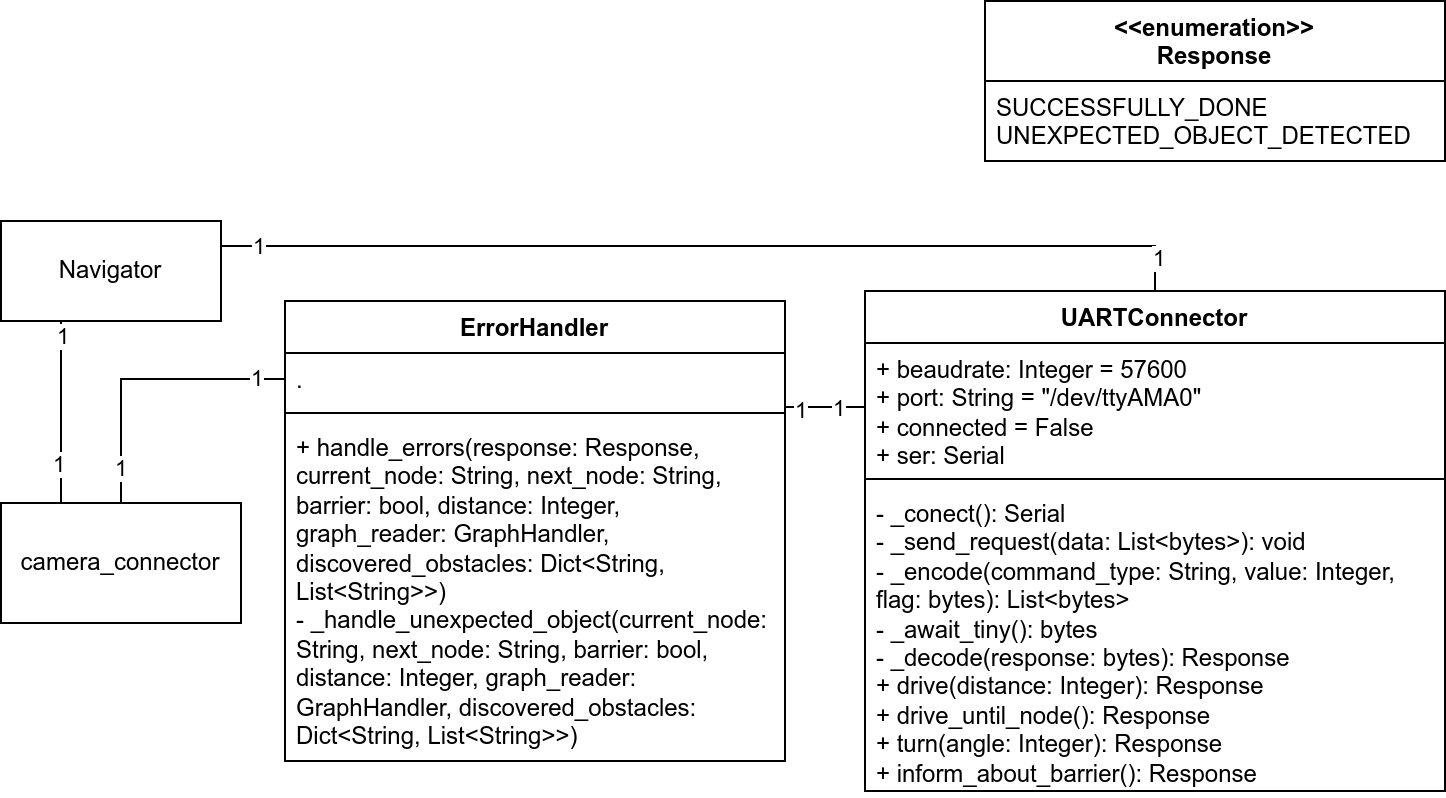
\includegraphics[width=\textwidth]{assets/IT/robot-sw-architecture-uart-connector.png}
\caption{UART Connector und Error Handler Klassendiagramm}
\label{fig:uart-connector-nav}
\end{figure}

Die UART-Connector Klasse  wird mithilfe der PySerial\footnote{\url{https://pypi.org/project/pyserial/}} Library implementiert. Diese kümmert sich selber um die Start- und Stop-Bits.
Die Verbindung wird mit diesen Zeilen aufgebaut:

\begin{verbatim}
beaudrate = 57600
port = "/dev/ttyAMA0"
self.ser = serial.Serial(self.port, self.beaudrate, timeout=1)
\end{verbatim}

Die Bewegungsinstruktionen werden, wie im Interface definiert, encoded. Es wird eine Liste mit 4 Bytes erstellt.
Diese Daten werden auf die serielle Verbindung geschrieben.
Danach wird gewartet, bis die Steuerung antwortet. Die Antwort wird wie in Tabelle \ref{table:statuscodes} decoded mit dem Response Enum.
Falls es einen 0 Statuscode (erfolgreich) gibt, wird normal weitergemacht. Falls ein andere Statuscode zurückgegeben wird, wird dieser dem ErrorHandler übergeben.

Der Errorhandler führt die Sequenz aus, die benötigt wird je nach Error.

Das Encoden der Nachrichten wurde mit mehreren Unittests getestet. Diese Unittests, sowie alle folgenden Unittests in der Navigation sind nach dem Muster `Arrange, Act, Assert'\footnote{\url{https://automationpanda.com/2020/07/07/arrange-act-assert-a-pattern-for-writing-good-tests/}} aufgebaut.

Im Arrange Teil wird hier festgelegt, was der Roboter machen soll und wie er antworten soll. Die Antwort wird gemocked\footnote{\url{https://microsoft.github.io/code-with-engineering-playbook/automated-testing/unit-testing/mocking/}} mithilfe von der Unittest Library.\footnote{\url{https://docs.python.org/3/library/unittest.mock.html}} Beispielsweise soll der Roboter -200cm fahren und die Antwort soll 0 sein, sprich, die Sequenz wurde richtig ausgeführt.

Im Act Teil wird die Funktion aufgerufen, die getestet wird. In diesem Beispiel ist das die `drive' Funktion.

Im Assert Teil wird getestet, ob die zurückgegebene Response korrekt decodiert wurde (von 0 zu SUCESSFULLY\_DONE) und ob die Funktion, die auf den \gls{tinyk22} schreibt, die richtigen Daten gesendet hat, was in diesem Fall ein Array mit folgendem Inhalt wäre:

\begin{verbatim}
# decimal values in Array get converted to Bytes when sent:
# 00000000, 00000000, 11001000 (200 to drive), 00000010 (drive backward)
[0, 0, abs(-200), 2]'
\end{verbatim}

Damit auch ohne Verbindung zu einem \gls{tinyk22} eine lauffähige Version verfügbar ist, wird beim Erstellen der UARTConnector Klasse geprüft, ob eine serielle Verbindung aufgebaut werden konnte. Wenn nicht, werden nach wie vor die alten Teile des Simulators verwendet. Dieser Zustand wird in der `connected' Variable festgehalten. Dies hilft beim Debuggen und Testen von einzelnen Modulen.


\newpage
%%%%%%%%%%%%%%%%%Epic 5%%%%%%%%%%%%%%%%%%%%%%%%%%%%%%%%%%%%%%%%%%%%%%%%%%%%%%%
\subsection{Hindernis umplatzieren}

Das Umplatzieren eines Hindernisses erfolgt in mehreren Stufen. Damit das Hindernis angehoben werden kann, wurde ein Greifer konstruiert und angebracht. Dies ist genauer aufgezeigt in Kapitel \ref{Greifer konstruieren}.

\subsubsection{Objekterkennung mit Ultraschall}

Die Barriere soll mit der Kamera erkannt werden, bevor der Roboter beginnt auf die Linie zu fahren. Der Raspberry Pi wird der Steuerung mitteilen, dass auf der nächsten Strecke eine Barriere zu erwarten ist. Der Roboter fährt dann langsamer als normalerweise los mit der Erwartung anzuhalten, wenn er 7cm vor sich das Objekt bemerkt. Diese Distanz sorgt dafür, dass sich der Roboter sicher drehen kann, ohne die Barriere umzustossen, jedoch die Distanz, die er langsam zum Hindernis zuruecklegt moeglichst kurz ist.

Falls die Kamera die Barriere nicht erkannt, aber trotzdem eine auf der Strecke ist, wird der Ultraschallsensor ein Objekt erkennen und der Navigation mitteilen, dass etwas im Weg steht. Die Navigation nutzt die Kamera, um herauszufinden, welches Objekt sich vor dem Roboter befindet. Wird dabei eine Barriere erkannt, fährt der Roboter noch naeher ran, um 7cm vor ihr zu sein und der Wegstell-Prozess wird gestartet, um das Hindernis aus dem Weg zu räumen. 

\subsubsection{Roboter drehen}

Der Roboter muss sich drehen können, um das Hindernis wegzustellen. Ebenfalls muss er sich drehen können, damit der Roboter sich ausrichten kann, um eine bestimmte Linie zu befahren. Die ist in dem folgenden Kapitel \ref{outgoing-lines} beschrieben.

In \acrshort{pren1} wurde geplant, dass der Roboter sich mit den Encodern dreht. Dabei sind jedoch immer wieder Probleme aufgetreten. Die Untersuchung davon ist im Anhang zu finden im Kapitel \nameref{drehen-encoder}.

Aus diesem Grund wurde entschieden ein Gyroskop zu verwenden.
 Ein Gyroskop reagiert auf Drehbewegungen, die durch die Corioliskraft verursacht wird. Die Corioliskraft bringt eine Masse ins Schwingen, so kann die Drehbewegung detektiert werden \parencite{zielke2025}. Dieser Sensor wird über \acrshort{iic} angesteuert, um die Messdaten auszulesen. 

Die Tests dazu sind im Anhang in Kapitel \nameref{drehen-gyro} zu finden. Nachdem die ersten Tests erfolgreich waren, wurde das Gyroskop fest auf den Roboter angeschlossen und montiert, wie in Abb. \ref{fig:Gyroskop auf dem Roboter} unten links zu sehen ist. Danach wurden Tests durchgeführt, ob das Gyroskop noch immer richtig misst, wenn der Roboter mit den Rädern und dem Motor dreht. Dies war erfolgreich.


\begin{figure}[H]
\centering
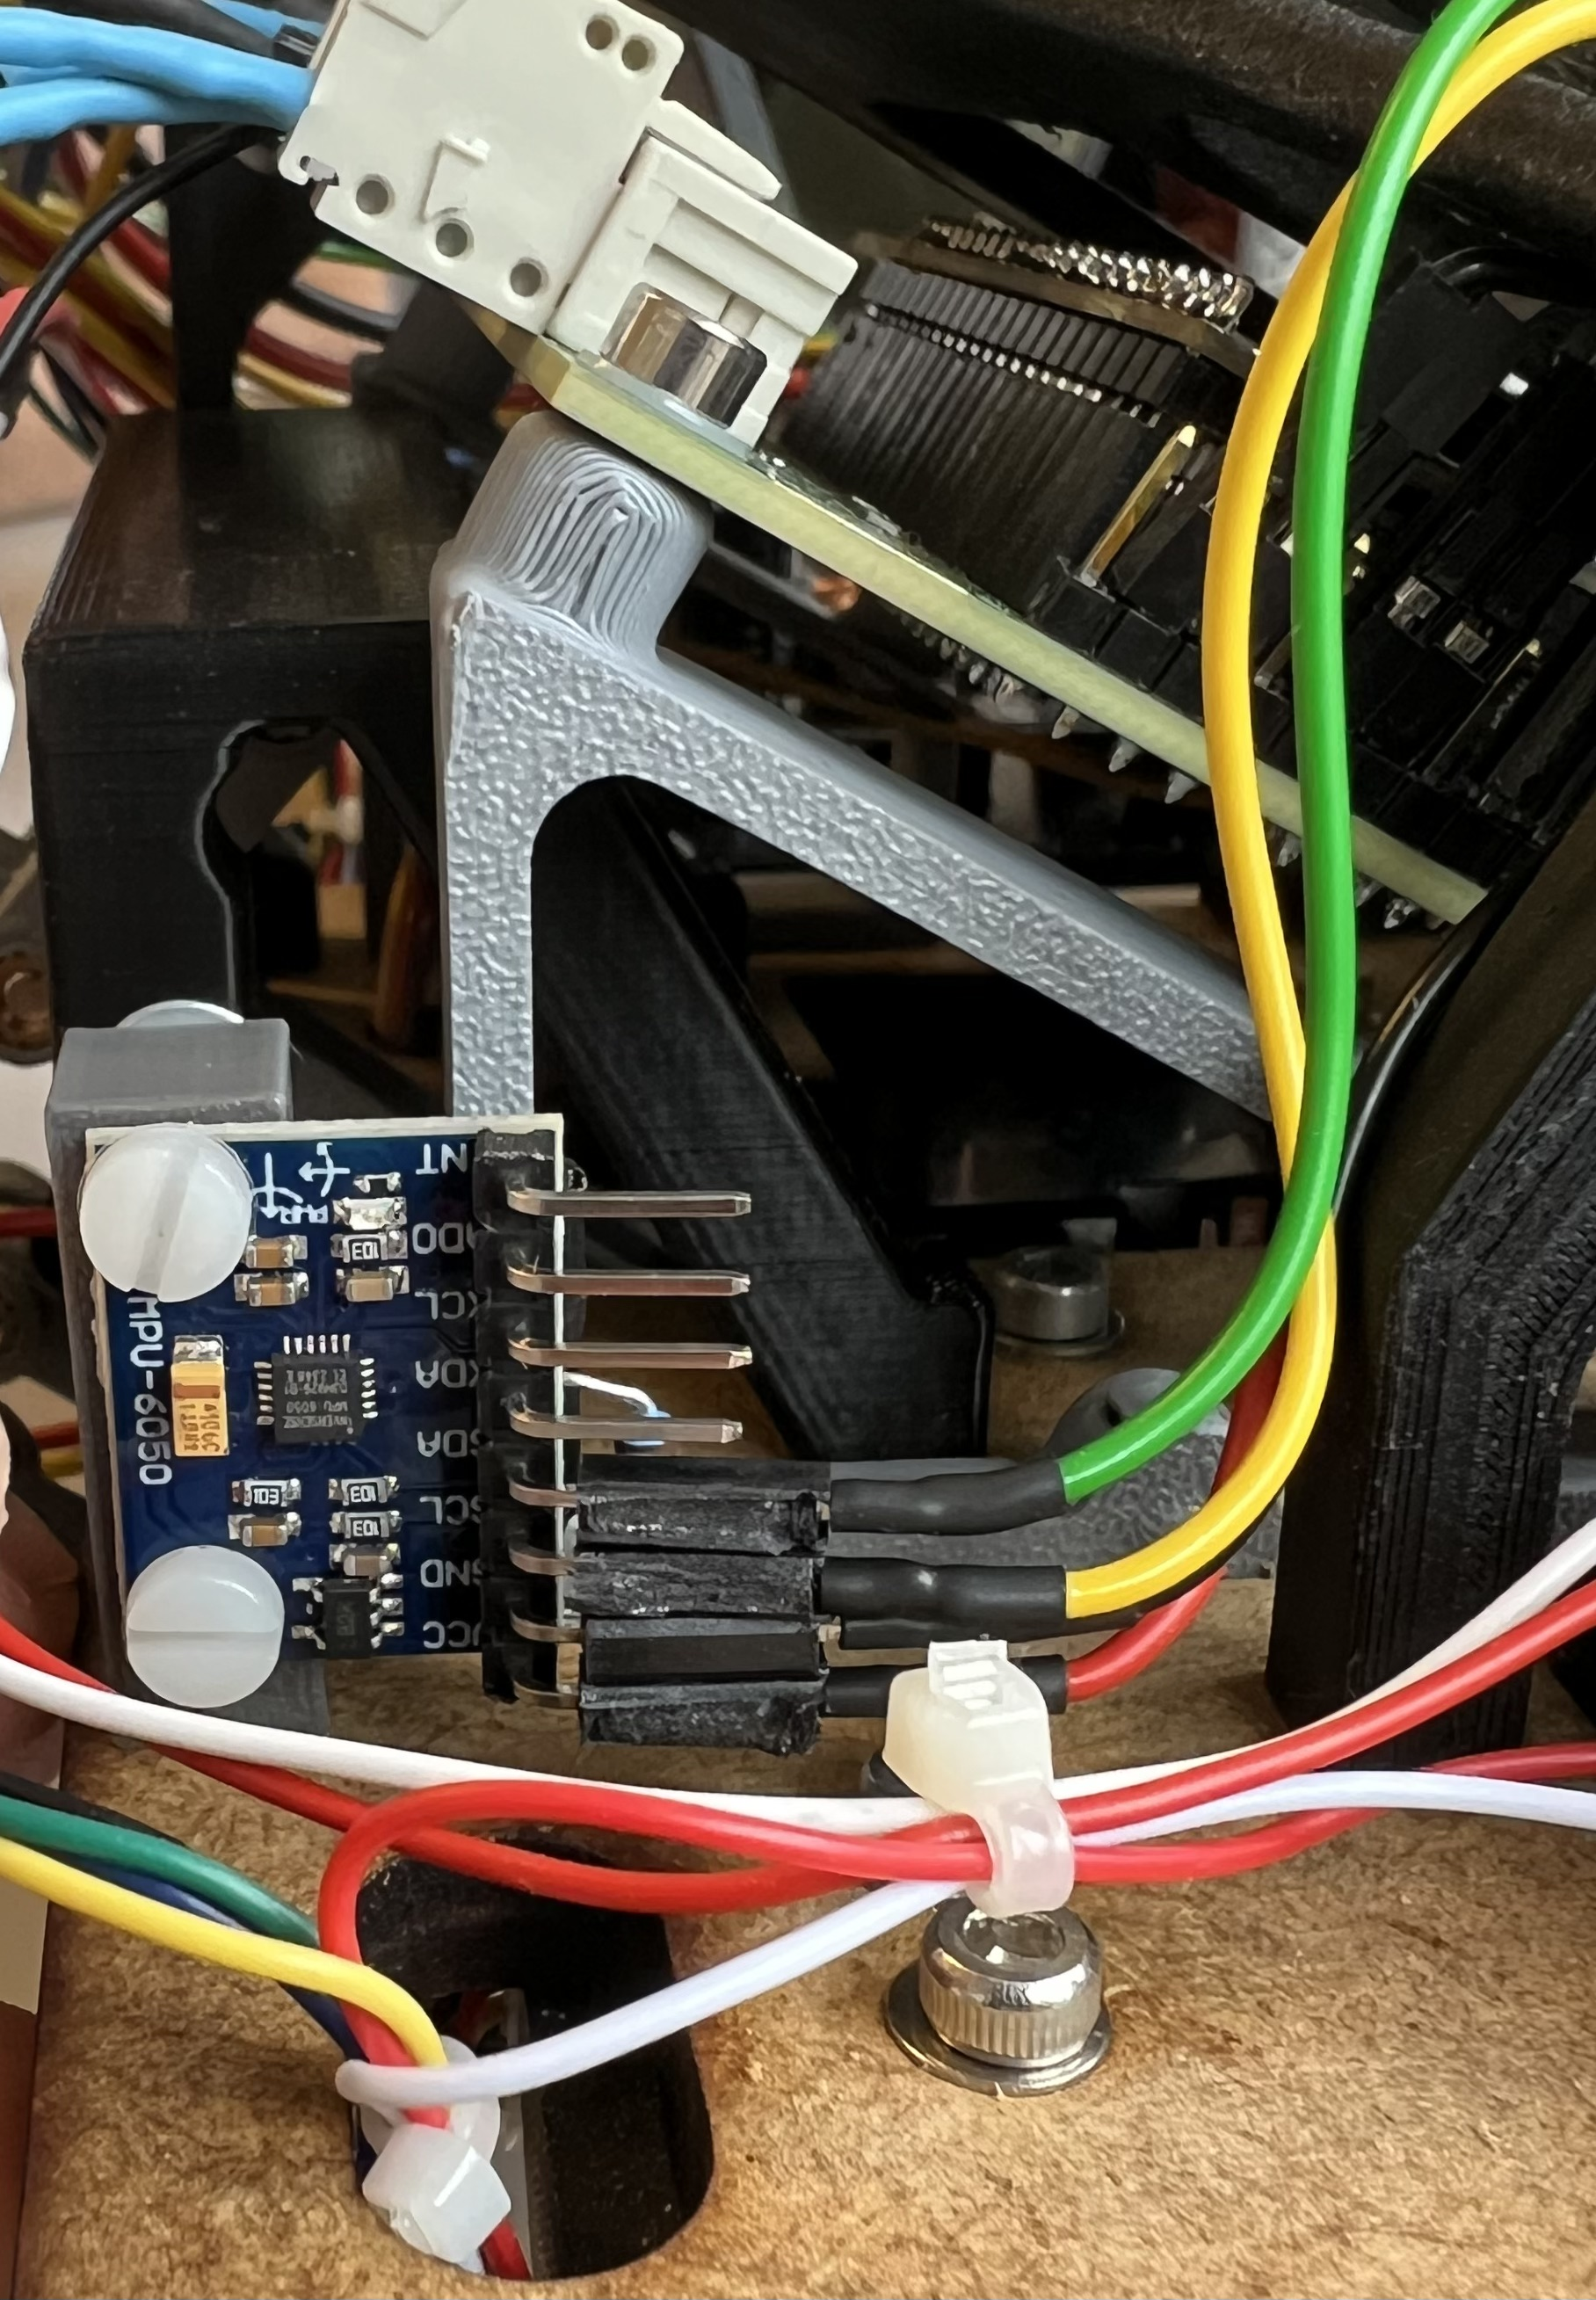
\includegraphics[width=5cm, height=7cm]{assets/ET/Gyroskop/Gyro_Montiert.jpeg}
\caption{Festmontierter Gyroskop auf dem Roboter}
\label{fig:Gyroskop auf dem Roboter}
\end{figure}

Es kann ein Befehl an die Steuerung gegeben werden mit dem gewünschten Winkel, in dem der Roboter sich drehen soll. Der Roboter dreht sich so lange, bis das Gyroskop misst, dass der Wert erreicht wurde, dann stoppt er.


\subsubsection{Servomotor für Greifer} 

Der Servomotor wurde bereits in Pren 1 getestet und dokumentiert. Durch die Ergebnisse von diesem Test konnte die Software erfolgreich implementiert werden.

TODO BILD

\subsubsection{Wegstellbefehl}

Falls der Roboter sich noch auf dem vorherigen Knoten befindet und die Kamera die Barriere erkannt hat, fährt er soweit, bis der Ultraschall die Barriere bemerkt auf 10cm Abstand. 
Falls die Kamera keine Barriere im Voraus erkennt und der Ultraschall ein Objekt, das als Barriere erkannt wird, erkennt, hält der Roboter ebenfalls 10cm zuvor.

Dann dreht das Fahrzeug sich um und fährt rückwärts auf die Barriere zu, bis der Endschalter am Greifer betätigt wird. Bei Betätigung wird das Fahrzeug gestoppt und der Greifer hebt das Hindernis an.
Nach dem erfolgreichen Anheben des Objekts, dreht sich das Fahrzeug zurück in seine ursprüngliche Ausrichtung. Anschliessend erfolgt eine Nachkorrektur der Position, um das Objekt wieder an derselben Position abzusetzen.

Der Wert der Nachkorrektur ist 12cm und wurde experimentell ermittelt. Diese Experimente sind im Anhang im Kapitel \nameref{hindernis-nachkorrektur} zu finden.

Nach der Nachkorrektur stellt der Roboter das Hindernis wieder ab und fährt, bis der nächste Knoten erkannt wird.


\newpage
%%%%%%%%%%%%%%%%%Epic 6%%%%%%%%%%%%%%%%%%%%%%%%%%%%%%%%%%%%%%%%%%%%%%%%%%%%%%%
\subsection{Auf Linie ausrichten}



\subsubsection{Ausgehende Linien erkennen}
\label{outgoing-lines}

Die eigenständige Software zum Erkennen ausgehender Linien wurde bereits in \acrshort{pren1} umgesetzt und getestet. In \acrshort{pren2} wurde diese Funktionalität in die zentrale Roboter-Software integriert. Abbildung \ref{fig:angle-reader-classdiagramm} zeigt das Klassendiagramm der dafür verantwortlichen Klasse \verb|AngleReader|.

\begin{figure}[H]
    \centering
    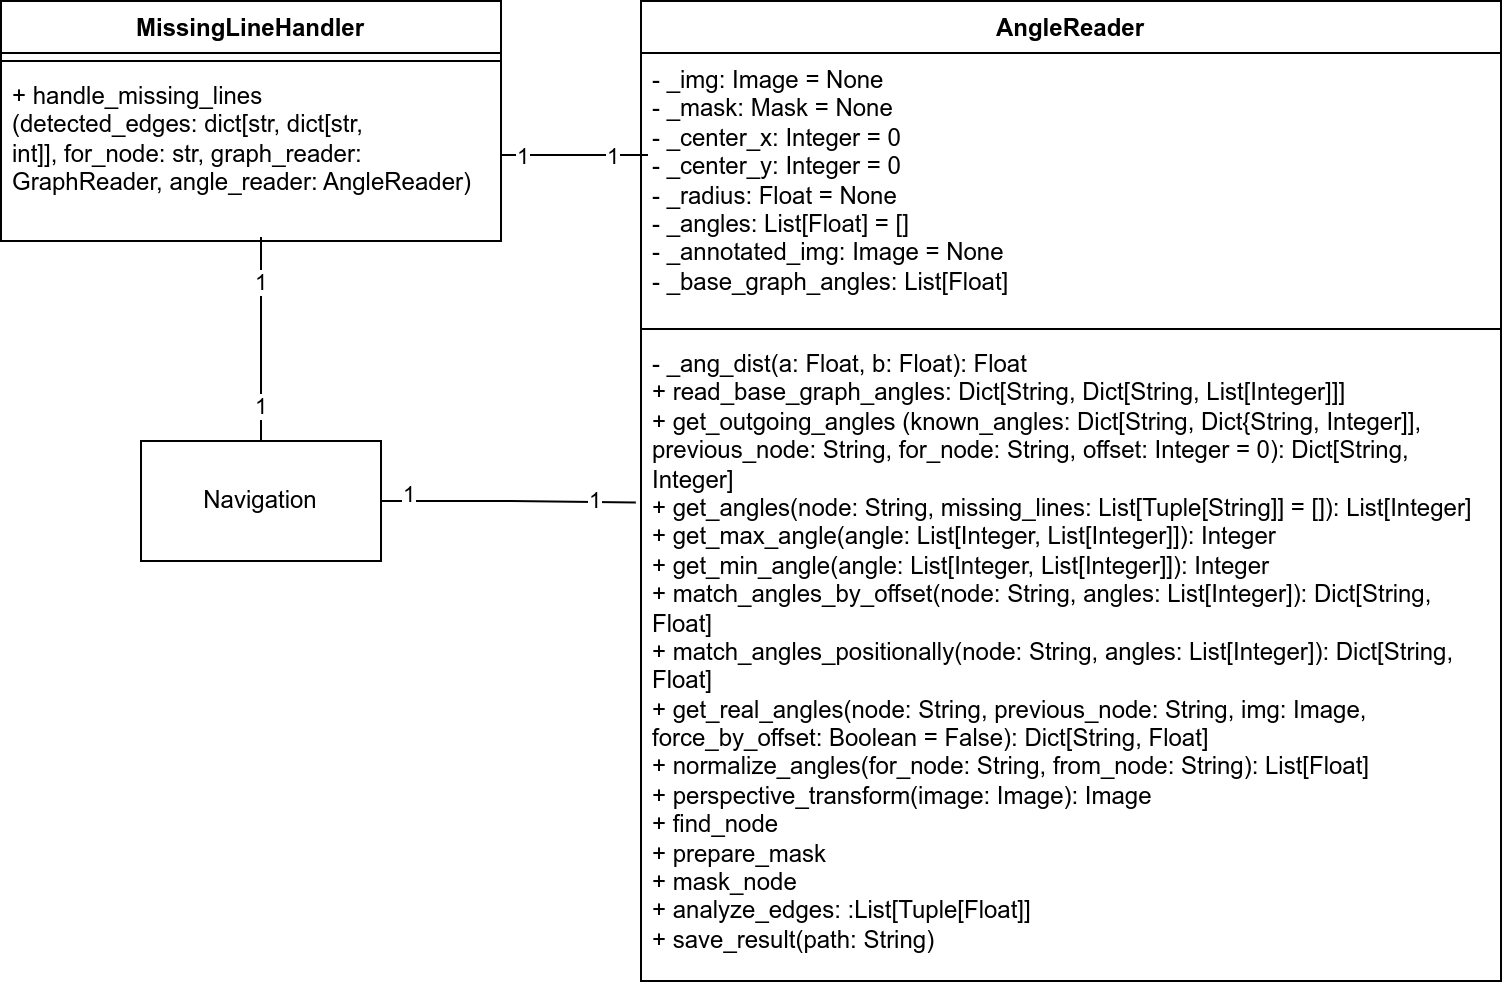
\includegraphics[width=1\linewidth]{assets/IT/robot-sw-architecture-node_reader_angles.png}
    \caption{Angle-Reader Klassendiagramm}
    \label{fig:angle-reader-classdiagramm}
\end{figure}

Die Klasse \verb|AngleReader| ist verantwortlich für das Erkennen und Zuordnen der ausgehenden Kanten eines Knotens anhand eines Bildes. Dabei kommen verschiedene Bildverarbeitungsschritte zum Einsatz: 
\begin{itemize}
    \item Perspektivtransformation zur Normalisierung der Bildansicht
    \item Erkennung des zentralen Knotens (Kreisform) mittels \verb|HoughCircles|
    \item Farbsegmentierung zur Isolation der Linien (Kanten)
    \item Analyse der Konturen zur Berechnung der Winkel der Linien relativ zur Knotenmitte
\end{itemize}

Die detektierten Winkel werden anschliessend mit den erwarteten Winkeln aus einer statischen YAML-Konfigurationsdatei (\verb|base_graph_angles.yml|) abgeglichen. Dies geschieht entweder über:
\begin{itemize}
    \item \textbf{Positionsbasiertes Matching}: Falls die Anzahl erkannter Linien mit der Anzahl erwarteter Linien übereinstimmt, werden die Winkel einfach nach ihrer Reihenfolge im Uhrzeigersinn zugeordnet.
    \item \textbf{Toleranz-basiertes Matching}: Falls eine oder mehrere Linie zu wenig erkannt wurden, wird versucht, die Winkel anhand eines bekannten Winkelbereichs (z.B. $60^\circ \pm 30^\circ$) zuzuordnen.
\end{itemize}

Die Klasse bietet zudem die Möglichkeit, das erkannte Ergebnis mit Winkeln und Konturen auf dem Originalbild zu annotieren und zu speichern, was die Debugging-Möglichkeiten deutlich verbessert. Eine Beispiel Ausgabe vom Knoten E ist in der nachfolgenden Abbildung \ref{fig:angle-reader-debug-output} ersichtlich.

\begin{figure}[H]
    \centering
    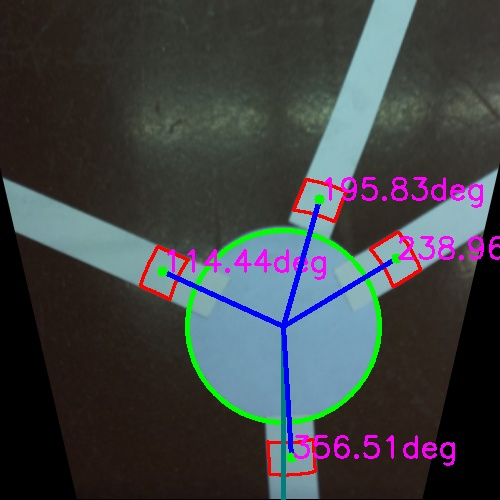
\includegraphics[width=0.5\linewidth]{assets/IT/250525_204610_test_annotated_angles_of_E.jpg}
    \caption{Debugging Ausgabe der Winkelerkennung vom Knoten E}
    \label{fig:angle-reader-debug-output}
\end{figure}

\textbf{Fehlende Linien erkennen und darauf reagieren}

Falls kein Knoten, zu viele Knoten, oder Kanten oder Kanten in falschen Winkelbereichen detektiert werden, wird folgender mehrstufiger Mechanismus aktiviert, um ein fehlerhaftes Einlesen auszuschliessen, und den Prozess der Winkelerkennung zu wiederholen:
\begin{enumerate}
    \item Der Roboter fährt 20cm zurück.
    \item Danach fährt er in kleinen Schritten vorwärts und macht dabei fortlaufend Bilder, um die Kanten erneut zu erkennen.
    \item Wird auch nach mehreren Versuchen keine vollständige Kantenstruktur erkannt, geht der Roboter davon aus, dass der Knoten nicht vollständig zugänglich oder die Markierungen beschädigt sind, oder er sich verirrt hat, also nicht auf einem Knoten steht, den er erwartet hat. (z.B. Beim traversieren einmal falsch abgebogen.)
    \item In diesem Fall wird der Knoten aus dem internen Graphen entfernt, der Roboter fährt zum vorherigen Knoten zurück und wählt eine alternative Route.
\end{enumerate}

    %%%%%%%%%%%%%%%%%Epic 7, 8, 9, 10%%%%%%%%%%%%%%%%%%%%%%%%%%%%%%%%%%%%%%%%%%%%%%%%%%%%%%%

\subsection{Objekte erkennen}

Dieses Kapitel behandelt die Methoden zur Objekterkennung. Zur Identifikation von Objekten auf dem Graphen, wurde ein YOLOv11-Modell eingesetzt, das speziell für diese Aufgabe trainiert wurde. Die erzielten Modellresultate werden vom Raspberry Pi ausgewertet, damit der Roboter die optimale Route wählen kann. Ergänzend dazu dient ein Ultraschallsensor als Backup-System zur Erkennung von Hindernissen, um die Sicherheit des Roboters zu erhöhen. 


\subsubsection{Kamera}
\label{camera-connector}

Zur Einbindung der Raspberry Pi Kamera in Python stellt Raspberry Pi die Bibliothek PiCamera2 zur Verfügung\footnote{\url{https://datasheets.raspberrypi.com/camera/picamera2-manual.pdf}}.
Abbildung \ref{fig:camera-connector-classdiagram} zeigt das Klassendiagramm des CameraConnector. Diese Klasse nutzt die PiCamera2-Bibliothek, um die Kamera zu konfigurieren und Fotos aufzunehmen. Darüber hinaus abstrahiert sie die Kamerakommunikation, sodass sowohl eine USB-Webcam als auch, wie in unserem Fall, die Raspberry Pi Kamera einheitlich angesprochen werden kann.

 \begin{figure}[H]
\centering
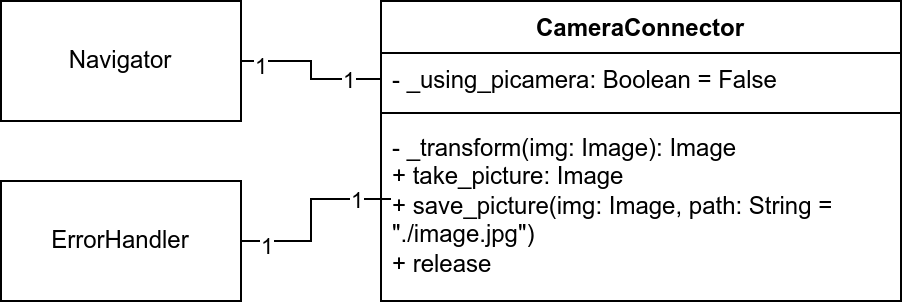
\includegraphics[width= \textwidth ]{assets/IT/robot-sw-architecture-camera-connector.png}
\caption{Kamera Modul}
\label{fig:camera-connector-classdiagram}
\end{figure}



\subsubsection{Ultraschall}
\label{ultraschall}

Zur Erhöhung der Betriebssicherheit ist das Fahrzeug mit einer redundanten Hinderniserkennung zusätzlich zu der Kamera ausgestattet. Diese erfolgt über einen Ultraschallsensor, der kontinuierlich die Entfernung zu Objekten im unmittelbaren Umfeld misst. Der Sensor ist direkt mit dem Mikrocontroller \gls{tinyk22} verbunden.

Die Messwerte werden in Echtzeit ausgewertet. Sobald ein Objekt in einer Distanz von weniger als 25 cm erkannt wird, hält der Roboter an, um Kollisionen zu vermeiden. Diese Distanz wurde gewählt, damit die Balance eingehalten wird zwischen 'zu viel' oder 'zu spät' erkennen. Es sollen nicht fälschlicherweise Objekte erkannt werden, jedoch sollen sie auch nicht zu spät erkannt werden. Dies ist auch deswegen so, da die Kamera benutzt wird, um das unerwartete Objekt zu deuten. Die Kamera braucht eine bestimmte Distanz, um eine mögliche Pylone zu erkennen, da diese möglichst ganz auf dem Bild sein sollte.

Es wird ein definierter Fehlercode generiert und über die serielle Schnittstelle an den Raspberry Pi übertragen. Der Raspberry Pi leitete entsprechende Massnahmen ein. Dies ist beschrieben in Tabelle \ref{table:statuscodes}.

Dies hilft dabei Risiko 12 (Objekte werden nicht erkannt) zu mitigieren, falls es passiert.



\subsubsection{YOLOv11-Model trainieren}

Damit der Roboter Pylonen, Knoten und Hindernissen erkennen kann, wurde ein \gls{yolo} Model trainiert.
Es wurden mehrere Models trainiert, die laufend miteinander verglichen wurden. Der Prozess wie das finale Model gewählt wurde, ist im Anhang in Kapitel \nameref{model-evaluation} zu finden.

Das Model, das verwendet werden wird, deutet die Bilder in ihrer Originalgrsse und hat über alle Klassen (Pylonen, Knoten, Hindernisse) gute Ergebnisse.

Die folgenden Bilder zeigen einige Bilder, die das Model annotiert hat. Darauf ist zu sehen, wie genau es die einzelnen Objekte erkennen kann.

\begin{figure}[H]
  \centering
    \begin{minipage}[b]{0.28\textwidth}
    \centering
    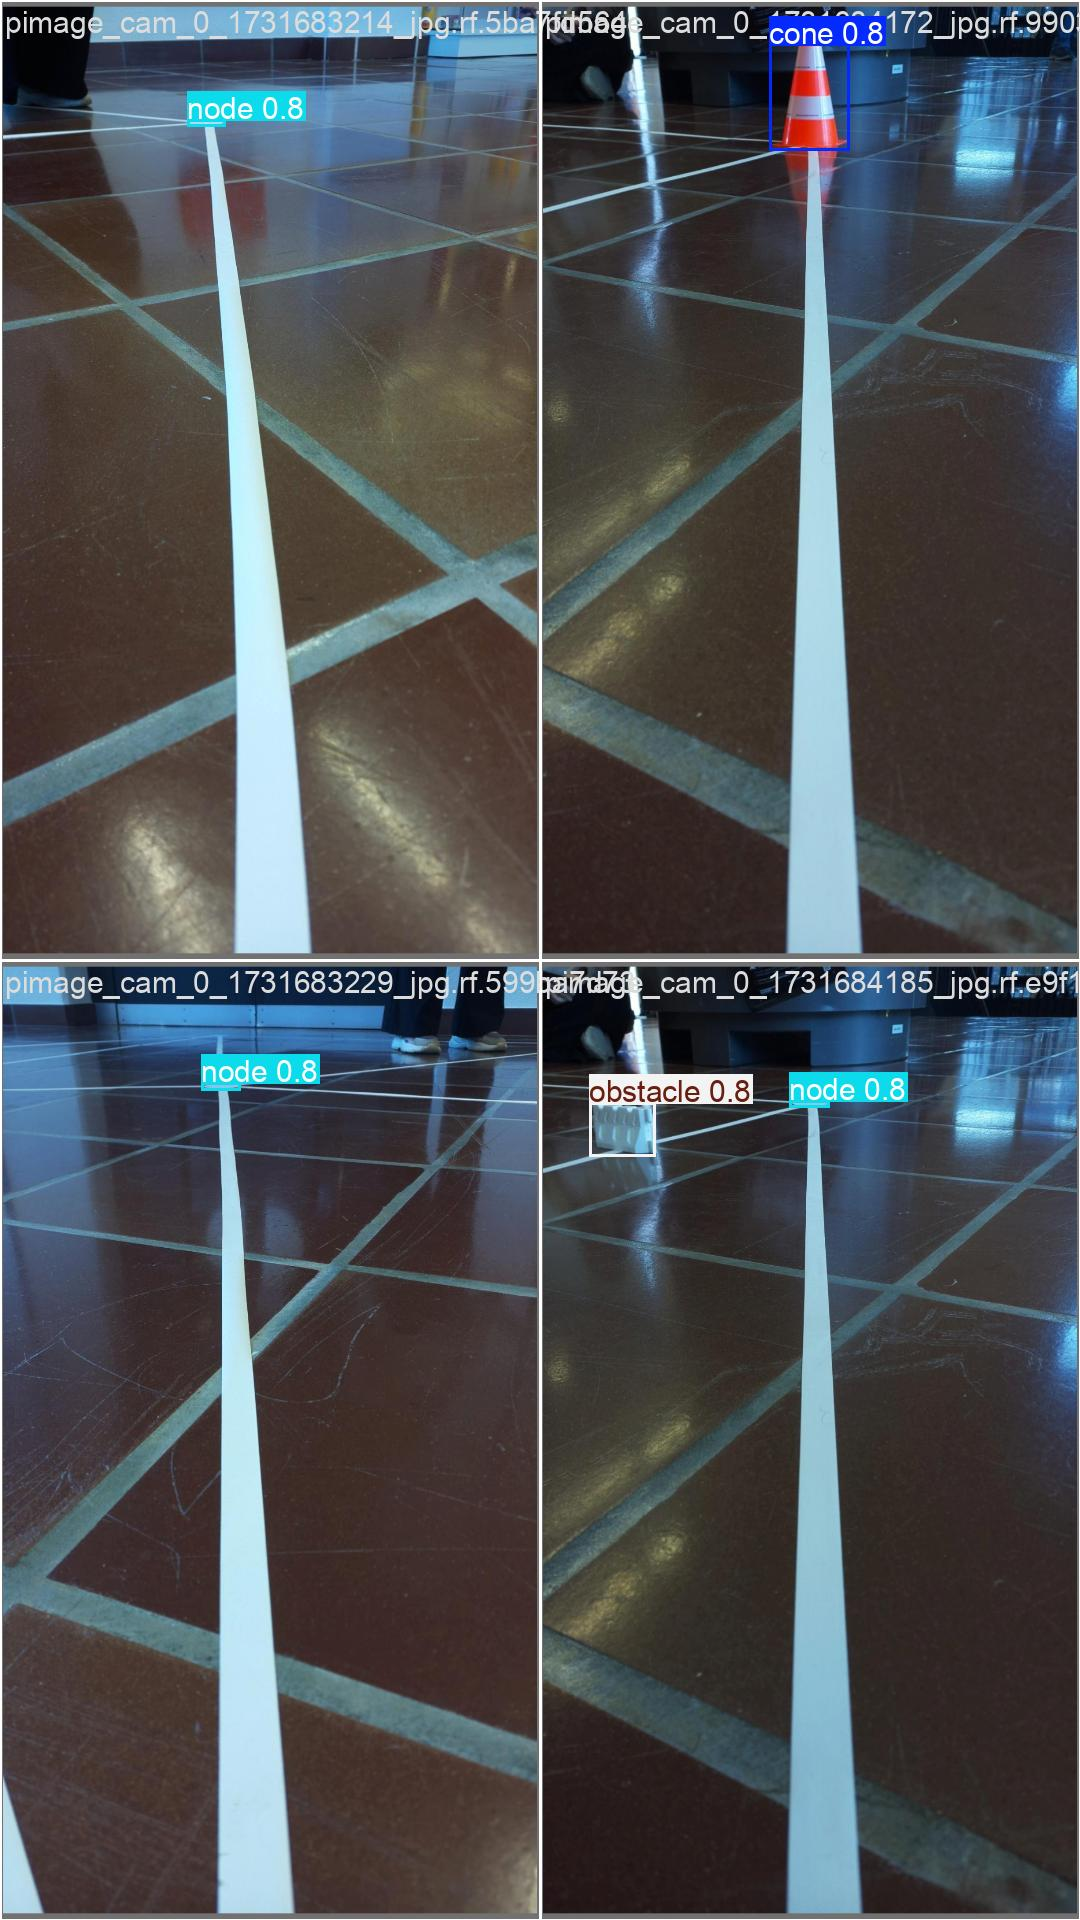
\includegraphics[width=\textwidth]{assets/IT/yolo/val_batch0_pred.jpg}
    \caption{Bilderkennung I}
    \label{fig:yolo-i}
  \end{minipage}
  \hfill
  \begin{minipage}[b]{0.28\textwidth}
    \centering
    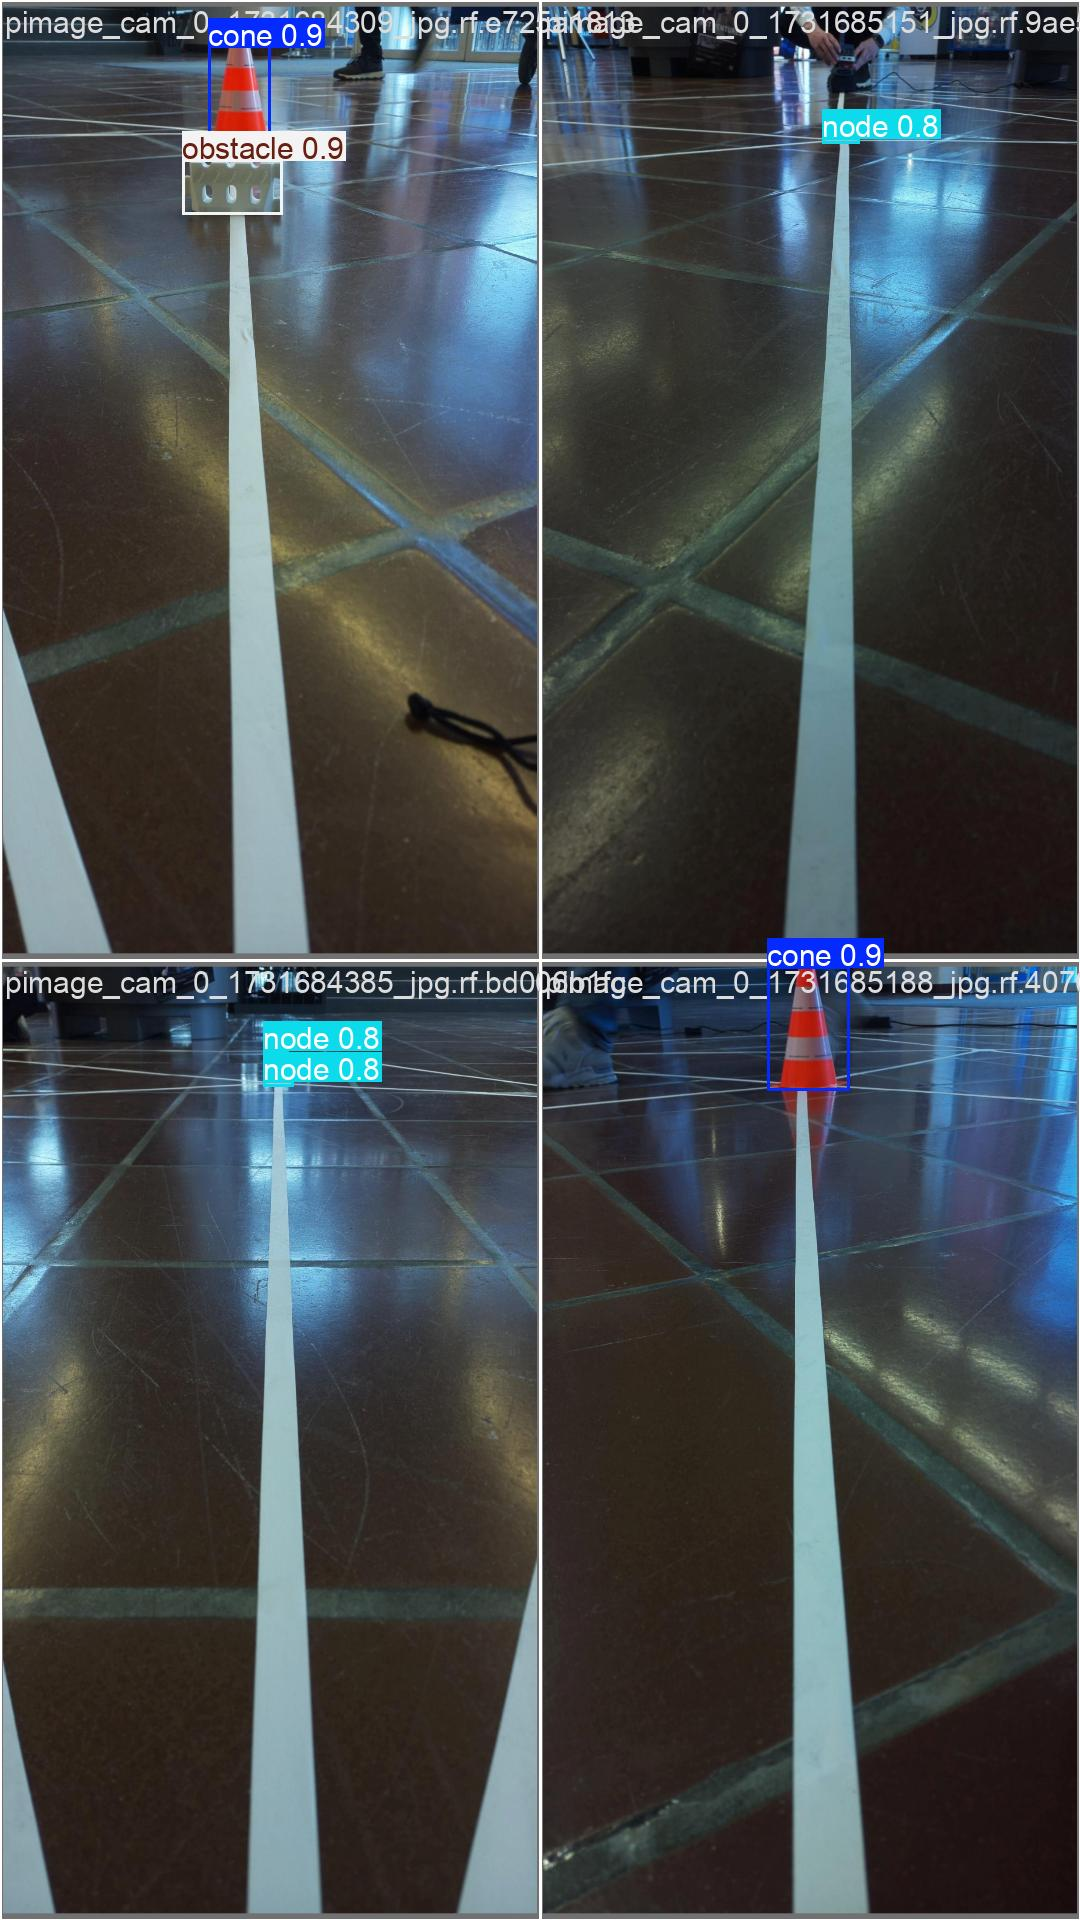
\includegraphics[width=\textwidth]{assets/IT/yolo/val_batch1_pred.jpg}
    \caption{Bilderkennung II}
    \label{fig:yolo-ii}
  \end{minipage}
    \hfill
  \begin{minipage}[b]{0.28\textwidth}
    \centering
    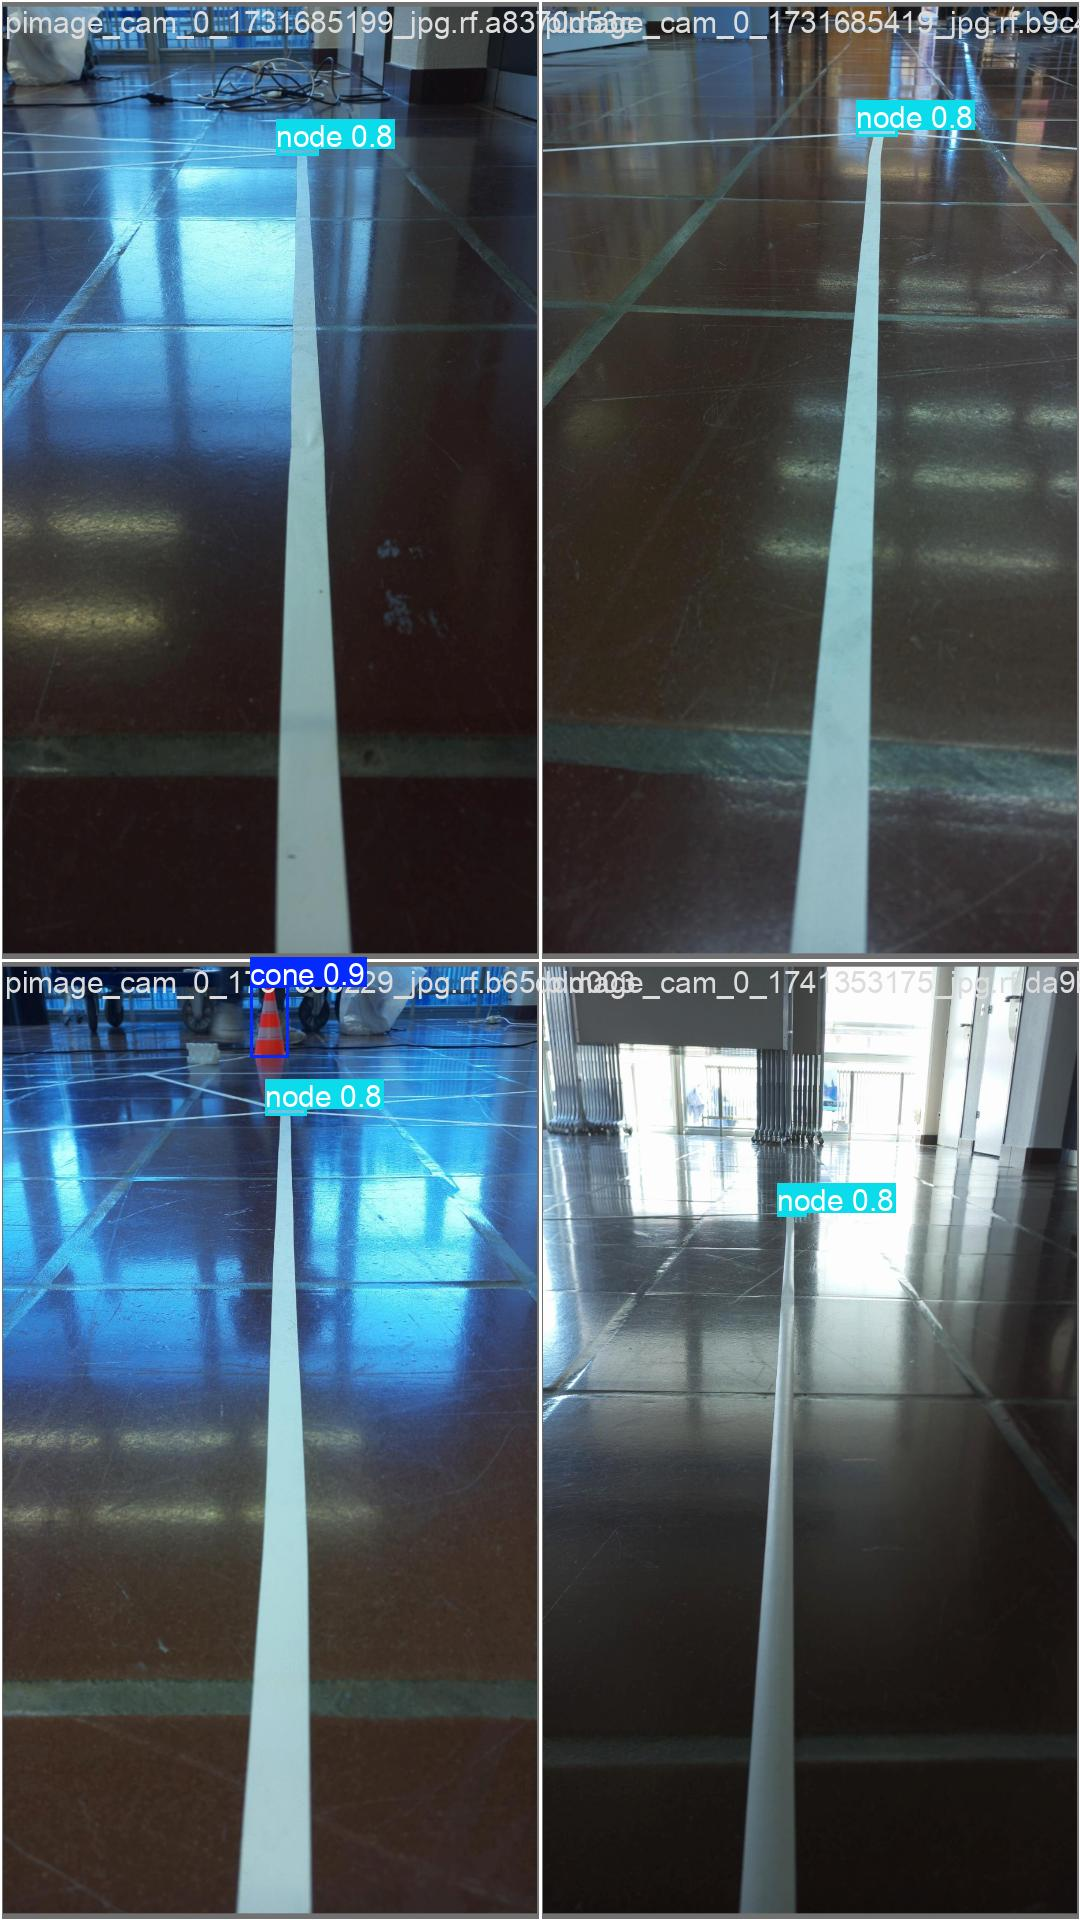
\includegraphics[width=\textwidth]{assets/IT/yolo/val_batch2_pred.jpg}
    \caption{Bilderkennung III}
    \label{fig:yolo-iii}
  \end{minipage}
\end{figure}

Auf den folgenden Bildern sind die Metriken aufgezeigt. Diese sind ebenfalls im Anhang im Kapitel \nameref{model-evaluation} genauer erklaert. Was hier sichtbar ist, ist zum einen der F1 Wert. Dieser ist besser, je höher er ist. Er ist hier fuer alle Klassen sehr hoch, was auf eine hohe Genauigkeit in den Detekierungen deutet. Ebenfalls ist die Consuion Matrix erkenntlich, diese zeigt welche Objekte das Model wie oft falsch oder richtig gedeutet hat. Das Model hat jede Pylone erkannt, hat sich zwei Knoten eingebildet und zwei Knoten verpasst. Mit den Algorithmen, die in dem nachfolgenden Kapitel \ref{model-results} beschrieben sind, die die Modelperformance stuetzen, sind diese Resultate ausgezeichnet. Ebenfalls ist der Lernverlauf des Models ersichtlich. Alle Graphen zeigen das gewünschte Muster. Die 6 Graphen links, die den Verlust in der Leistung (falsche Deutungen) darstellen, sind exponentiell fallend. Das heisst, dass das Modell mit jeder Iteration mehr gelernt hat und nicht irgendwann gestoppt hat oder schlechter wurde. Die 4 Graphen auf der rechten Seite zeigen, wie viel das Model gelernt, diese steigen und flachen dann ab. Dies ist ebenfalls das Muster, das bei einem guten Model erwartet wird.\cite{model-performance}

\begin{figure}[H]
  \centering
    \begin{minipage}[b]{0.3\textwidth}
    \centering
    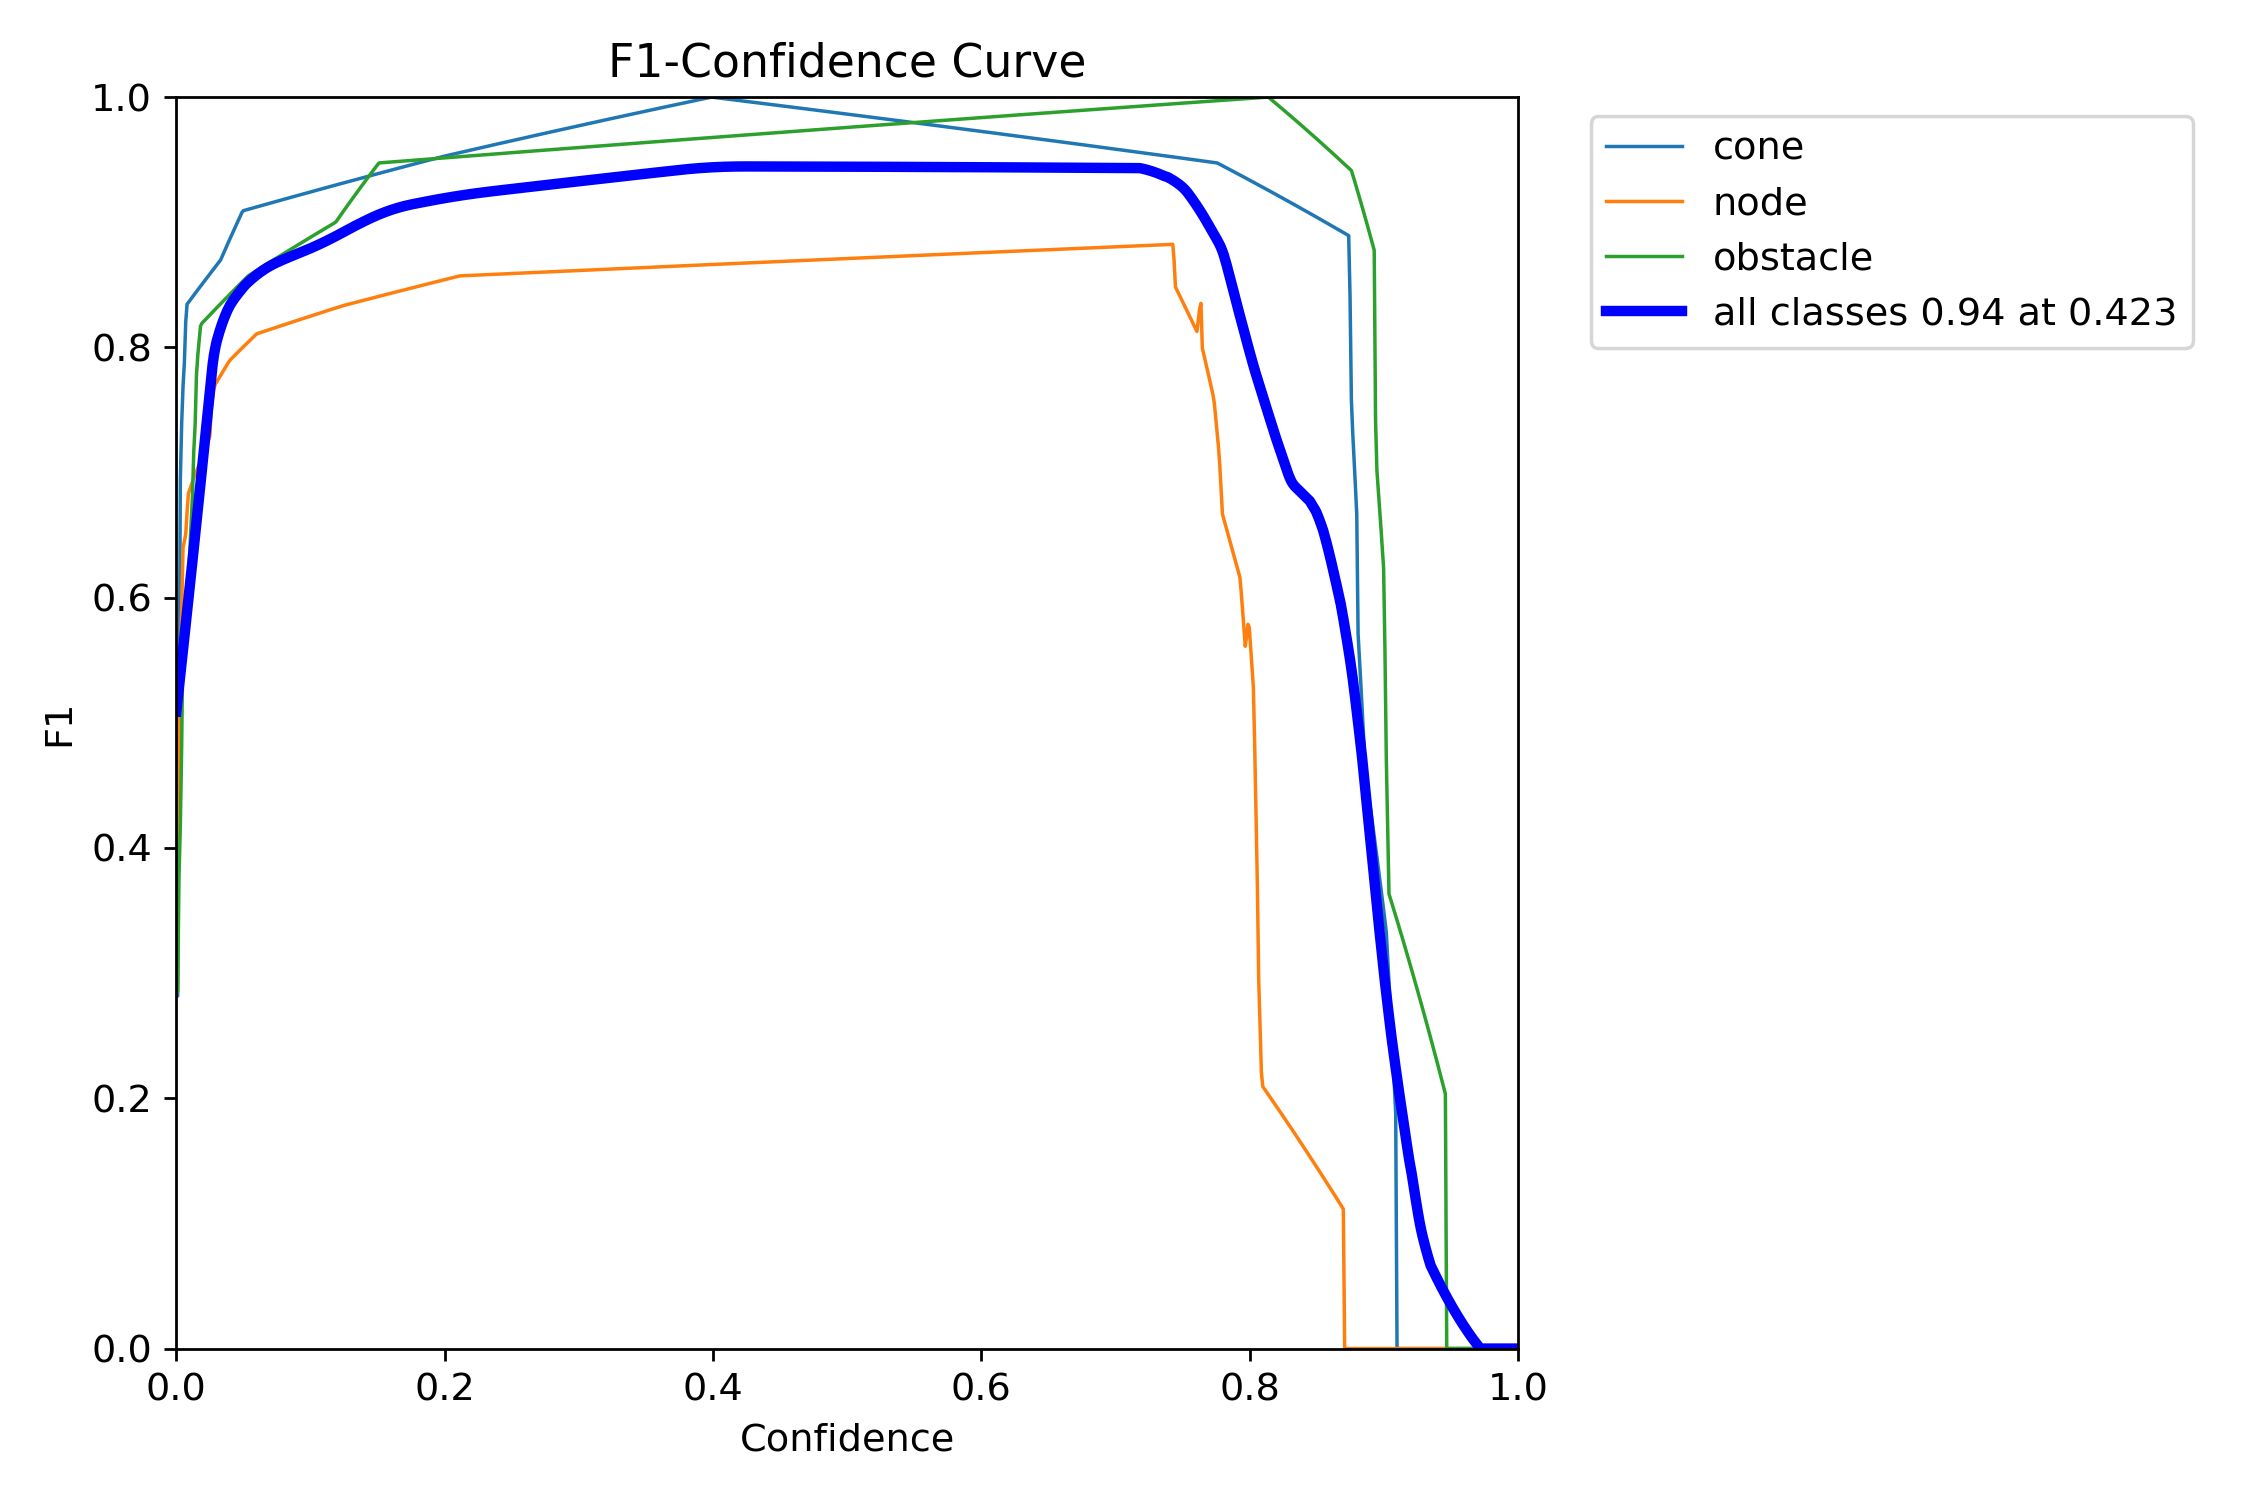
\includegraphics[width=\textwidth]{assets/IT/yolo/F1_curve.png}
    \caption{F1 Kurve}
    \label{fig:f1}
  \end{minipage}
  \hfill
  \begin{minipage}[b]{0.3\textwidth}
    \centering
    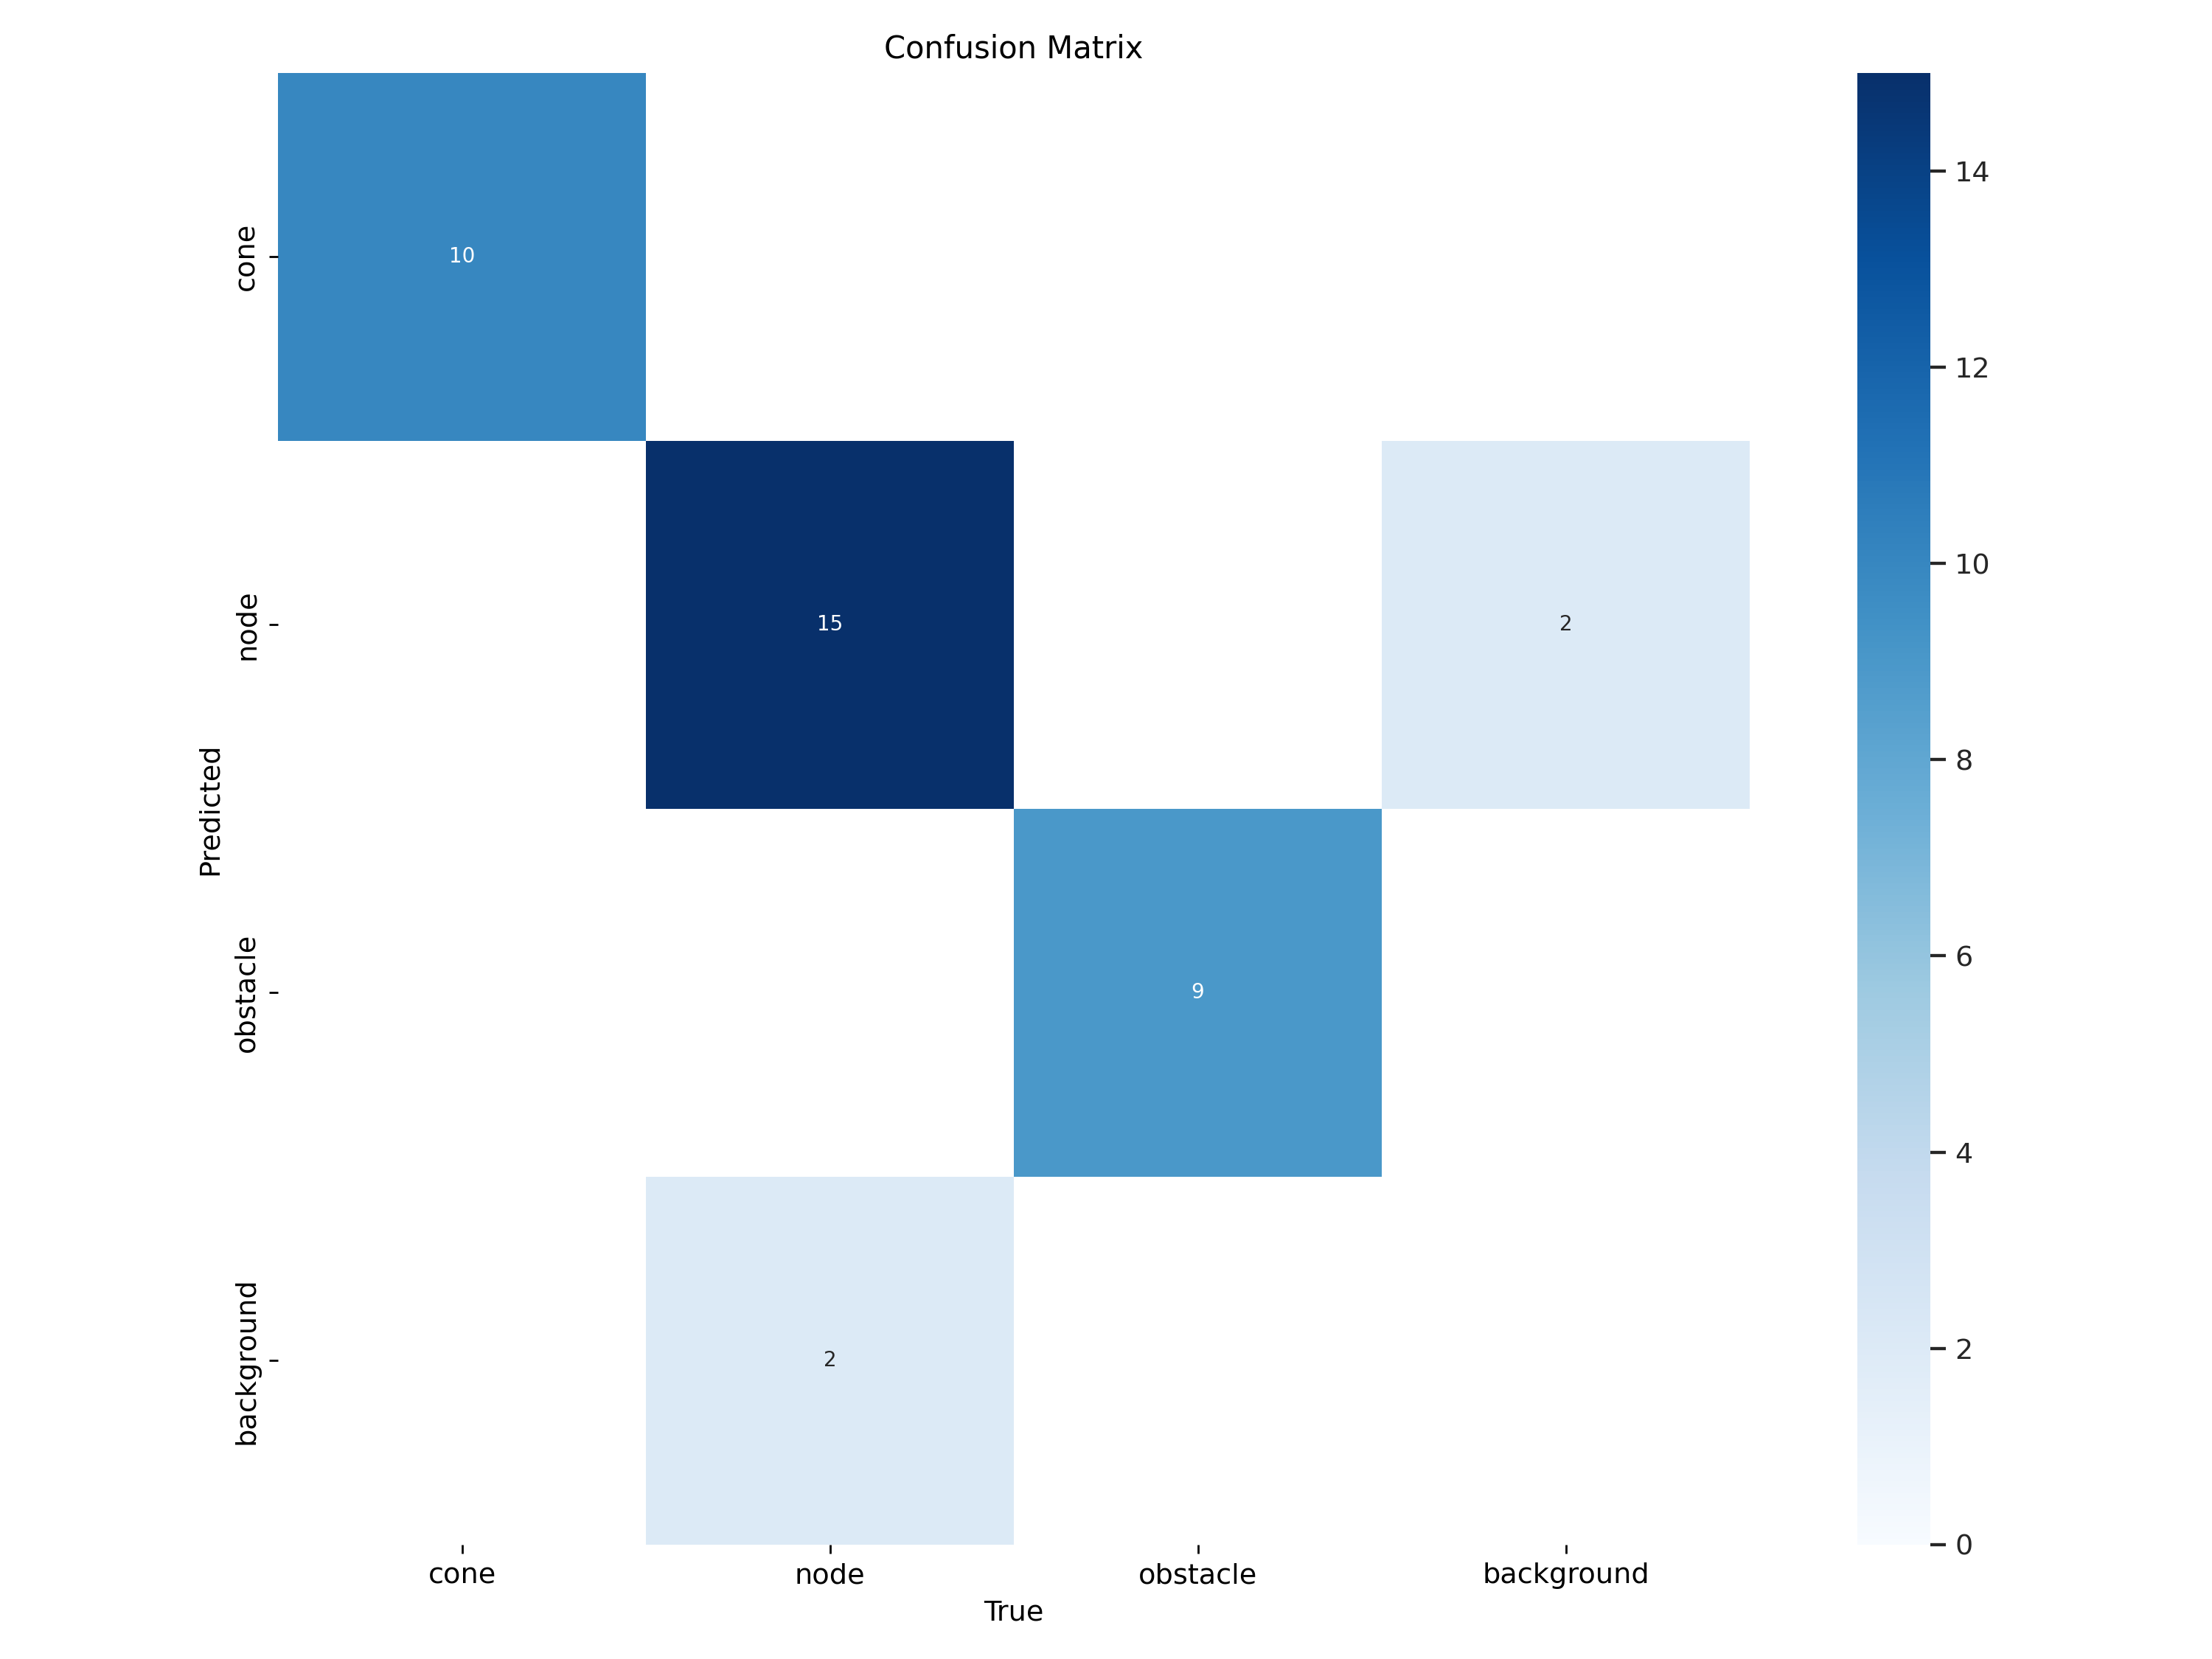
\includegraphics[width=\textwidth]{assets/IT/yolo/confusion_matrix.png}
    \caption{Confusion Matrix}
    \label{fig:conf-matrix}
  \end{minipage}
    \hfill
  \begin{minipage}[b]{0.3\textwidth}
    \centering
    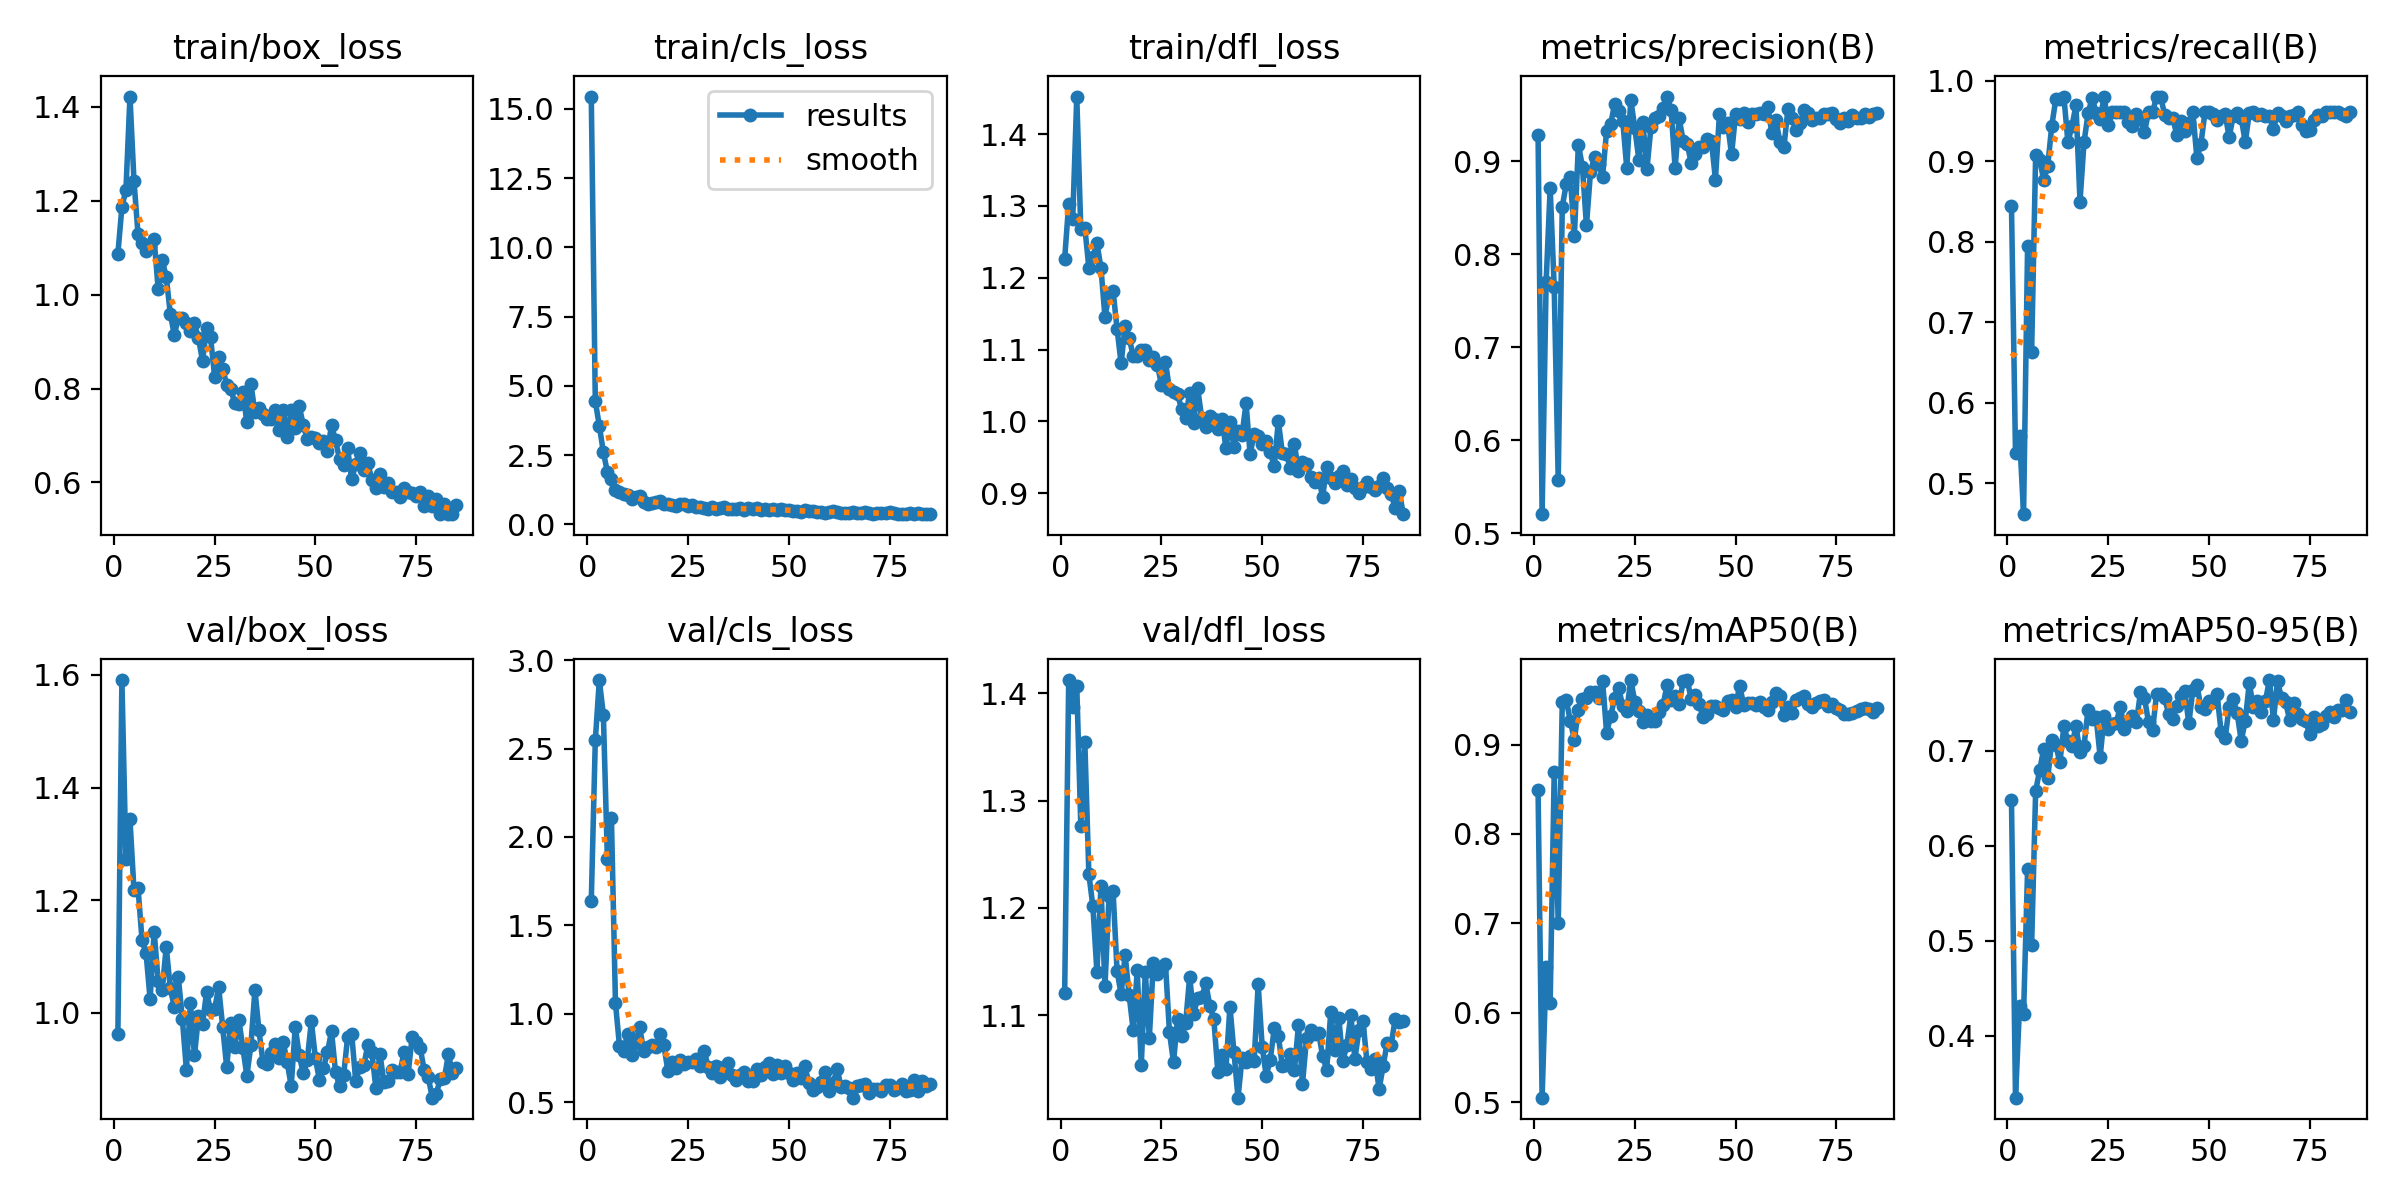
\includegraphics[width=\textwidth]{assets/IT/yolo/results.png}
    \caption{Lernverlauf}
    \label{fig:results-lernverlauf}
  \end{minipage}
\end{figure}

\subsubsection{YOLOv11 Model konvertieren}
\label{convert-yolo}

Es gibt Methoden, um die .pt Datei, die das Model enthaelt und verwendet wird, um Objekte zu erkennen, zu transformieren in ein anderes Format, damit auf Embedded Systems und somit auch auf Raspberry Pi's die Bilderkennung schneller durchgeführt werden kann.

Drei Möglichkeiten wurden betrachtet und verglichen:
TODO add sources for each \& akronyum
\begin{enumerate}
    \item Caffe2: In der Vergangenheit sehr geeignet, heutzutages mit PyTorch zusammengefügt und existiert nicht mehr auf diese Weise.
    \item NCNN: Sehr gute Performance für ARM Geräte (u.a. Raspberry Pi), sehr wenig Abhängigkeiten, einfache Transformation.
    \item ONXX: Geeignet für  Cross-Plattform Fälle, gute Austauschbarkeit des Models, flexibel, viele Abhängigkeiten.
\end{enumerate}

Es wird NCNN gewählt, da dies perfekt für den Use Case mit einem Raspberry Pi passt. Das erstellte .pt File kann mit der ultralytics Bibliothek transformiert werden:

\begin{verbatim}
yolo export model=best.pt format=ncnn
\end{verbatim}

Das Resultat ist ein Ordner, der gleich verwendet werden kann, wie das .pt File: Die Ultralytics Library erwartet den Pfad zu der Datei, respektive dem Ordner und baut daraus das YOLO Model, das verwendet werden kann in Python. Mit der Transformation wurde das Risiko 3: 4 Minuten reichen nicht für einen Durchgang, weiter gemindert. Auf dem Raspberry Pi, kann die Bilderkennung pro Bild konstant unter einer Sekunde gehalten werden.

\subsubsection{Modelresultate auswerten}
\label{model-results}

Um die Modelresultate auszuwerten wurde das Model in den Ordner der Navigation kopiert und es wurde eine ObjectDetector Klasse und ein Object Enum erstellt, gezeigt im Klassendiagramm \ref{fig:nav-object-detector}.

 \begin{figure}[H]
\centering
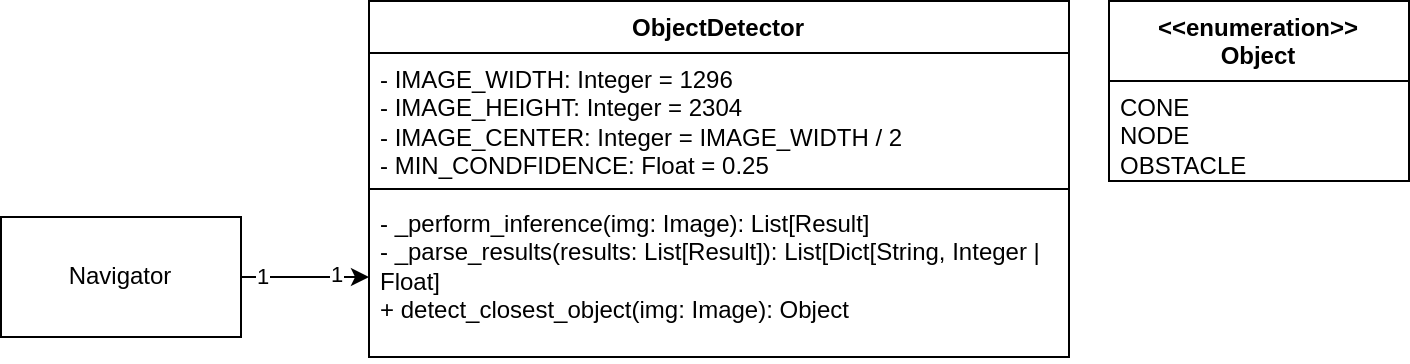
\includegraphics[width= \textwidth ]{assets/IT/robot-sw-architecture-object-detector.png}
\caption{Object Detector Modul}
\label{fig:nav-object-detector}
\end{figure}

Diese ObjectDetector Klasse ladet das Model bei der Instanzierung und wird aufgerufen, wenn ein Nachbarsknoten geprüft werden soll und führt einen Prozess von drei Schritten durch:

\begin{enumerate}
    \item Inference (Objekterkennung).
    \item Resultat parsen.
    \item Nächstes Objekte vor dem Roboter finden.
\end{enumerate}

Im Teil der Inference wird ein Bild an das Model gegeben. Dabei sollen nur die erkannten Objekte zurückgegeben werden, die mit einer definierten prozentualen Gewissheit erkannt wurden. Diese Gewissheit ist als Konstante definiert auf 0.4. Aus der F1 Kurve in Abbildung \ref{fig:f1} kann gelesen werden, dass die Pylone bei 0.4 die besten Resultate hat. Knoten und Pylone sind recht konstant und haben dort ebenfalls sehr genaue Resultate. Dadurch, dass dieser Wert erhöht wurde von dem Standardwert, kann das Risiko 7 (Ein Objekt wird fälsch-
licherweise erkannt) damit vermindert werden: Das Modell muss sich sicherer sein als dies standardmässig der Fall ist, damit die Deutung akzeptiert wird.

Diese Resultate werden dann geparsed, sodass alle erkannten Objekte mir ihrer ID, mit der Confidence, mit der sie erkannt wurden, und mit ihrem Standort auf dem Bild zurückgegeben werden.

Aus dieser Liste werden nun alle Objekte betrachtet, die sich auf der Mittellinie des Bildes befinden. Somit kann sichergestellt werden, dass nicht versehentlich Objekte, die sich nicht auf der Fahrbahn befinden, gespeichert werden und auch Risiko 7 (Objekte werden fälschlicherweise erkannt) kann so mitigiert werden. Die Mittellinie wird berechnet aus der Breite des Bildes. Die Objekte auf der Mittellinie werden sortiert nach ihren Koordinaten auf dem Bild. Das erste Element in dieser Liste ist das nächste Objekt zum Roboter. Die ID des Objektes, die vom Model zurückgegben wird, korrespondiert mit der ID des erstellten Enums, damit das erkannte Objekt als Enum zurückgegeben wird.

In folgenden Fällen wird nicht einfach das nächste Objekt zurückgegeben:

\begin{itemize}
    \item Falls das nächste Objekt eine Barriere und das zweitnächste eine Pylone ist. In diesem Fall wird zurückgegeben, dass eine Pylone das nächste Objekt ist, da dieser Knoten sowieso nicht befahrbar ist und aus dem internen Graph entfernt werden soll.
    \item Falls kein Objekt erkannt wurde, wird ein Knoten zurückgegeben. Es ist weniger wahrscheinlich, dass eine Barriere oder ein Pylon verpasst werden, als dass ein Knoten nicht erkannt wird. Somit wird Risiko 2 (Knoten werden nicht erkannt) behandelt. Der Ultraschall kann trotzdem Objekte noch erkennen, falls ein Objekt verpasst wurde. Es ist ein kleineres Problem ein Objekt zu verpassen, als sich eines einzubilden und fälschlicherweise Strecken zu entfernen. Durch den Ultraschall werden Risiko 12 und 1 (Objekte werden nicht erkannt) mitigiert.
\end{itemize}

Die folgenden Abbildungen veranschaulichen das Prinzip. Diese Bilder haben die einzelnen Objekte, die das Model erkannt hat mit Boxen annotiert. Die Bildunterschrift zeigt, welche Objekte zurueckgegeben werden basierend auf dem Algorithmus, der zuvor erklaert wurde. Wenn es keine Box annotiert haette, wuerde ebenfalls ein Knoten zurueckgegeben werden.

\begin{figure}[H]
  \centering
    \begin{minipage}[b]{0.23\textwidth}
    \centering
    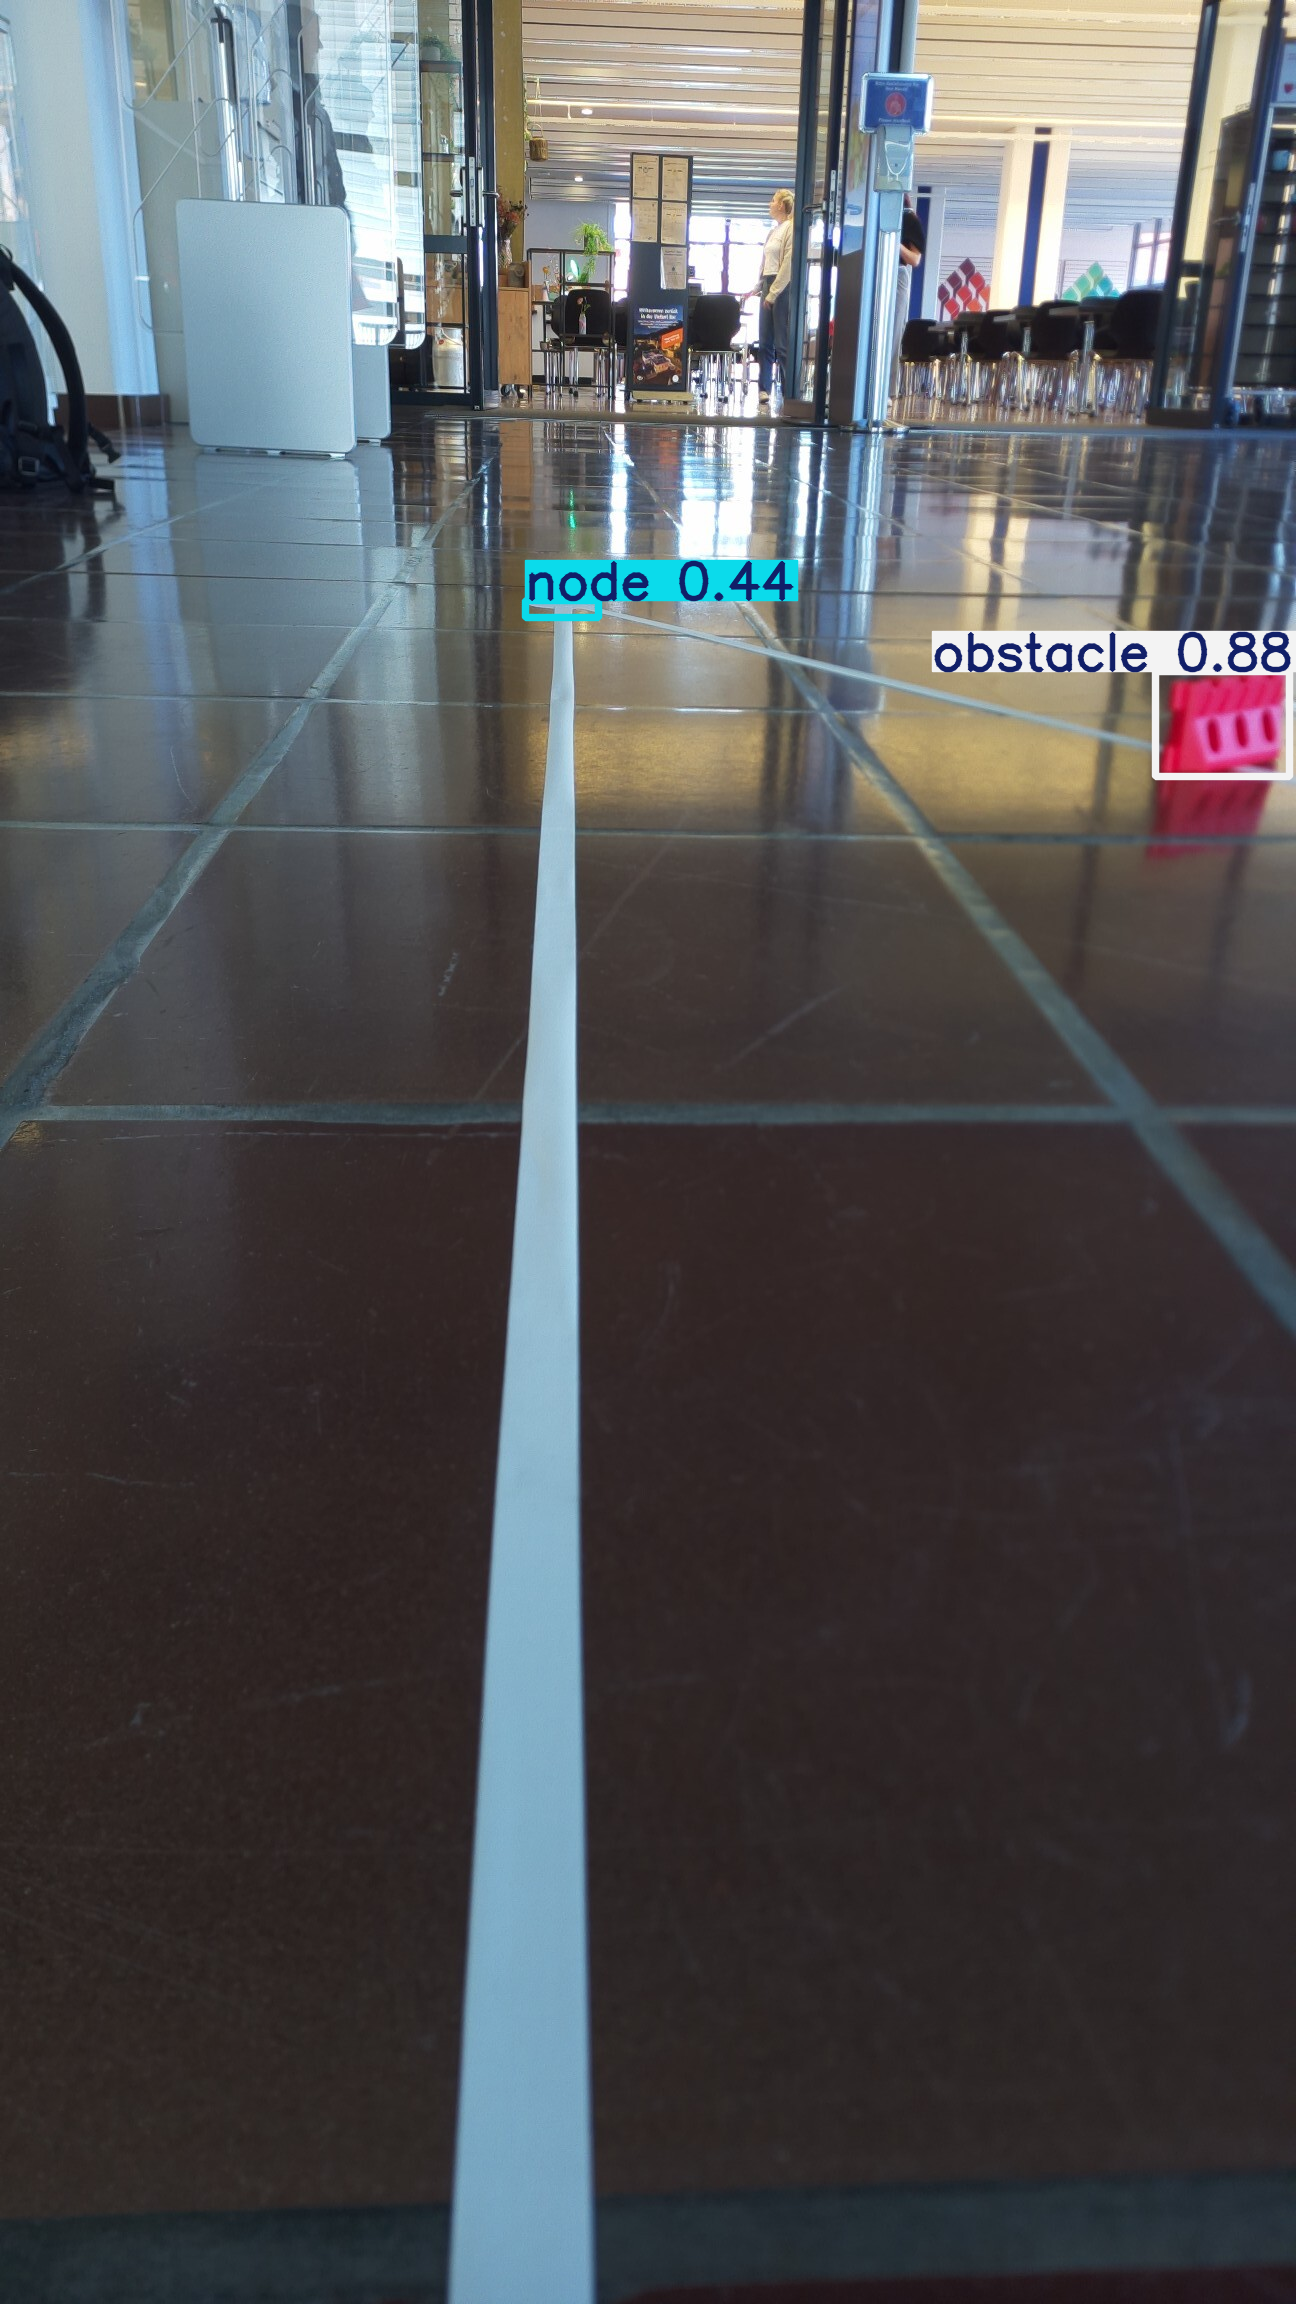
\includegraphics[width=\textwidth]{assets/IT/testing/yolo/node-obst-on-the-side_annot.png}
    \caption{Returned Knoten}
    \label{fig:expl-algo-1}
  \end{minipage}
  \hfill
  \begin{minipage}[b]{0.23\textwidth}
    \centering
    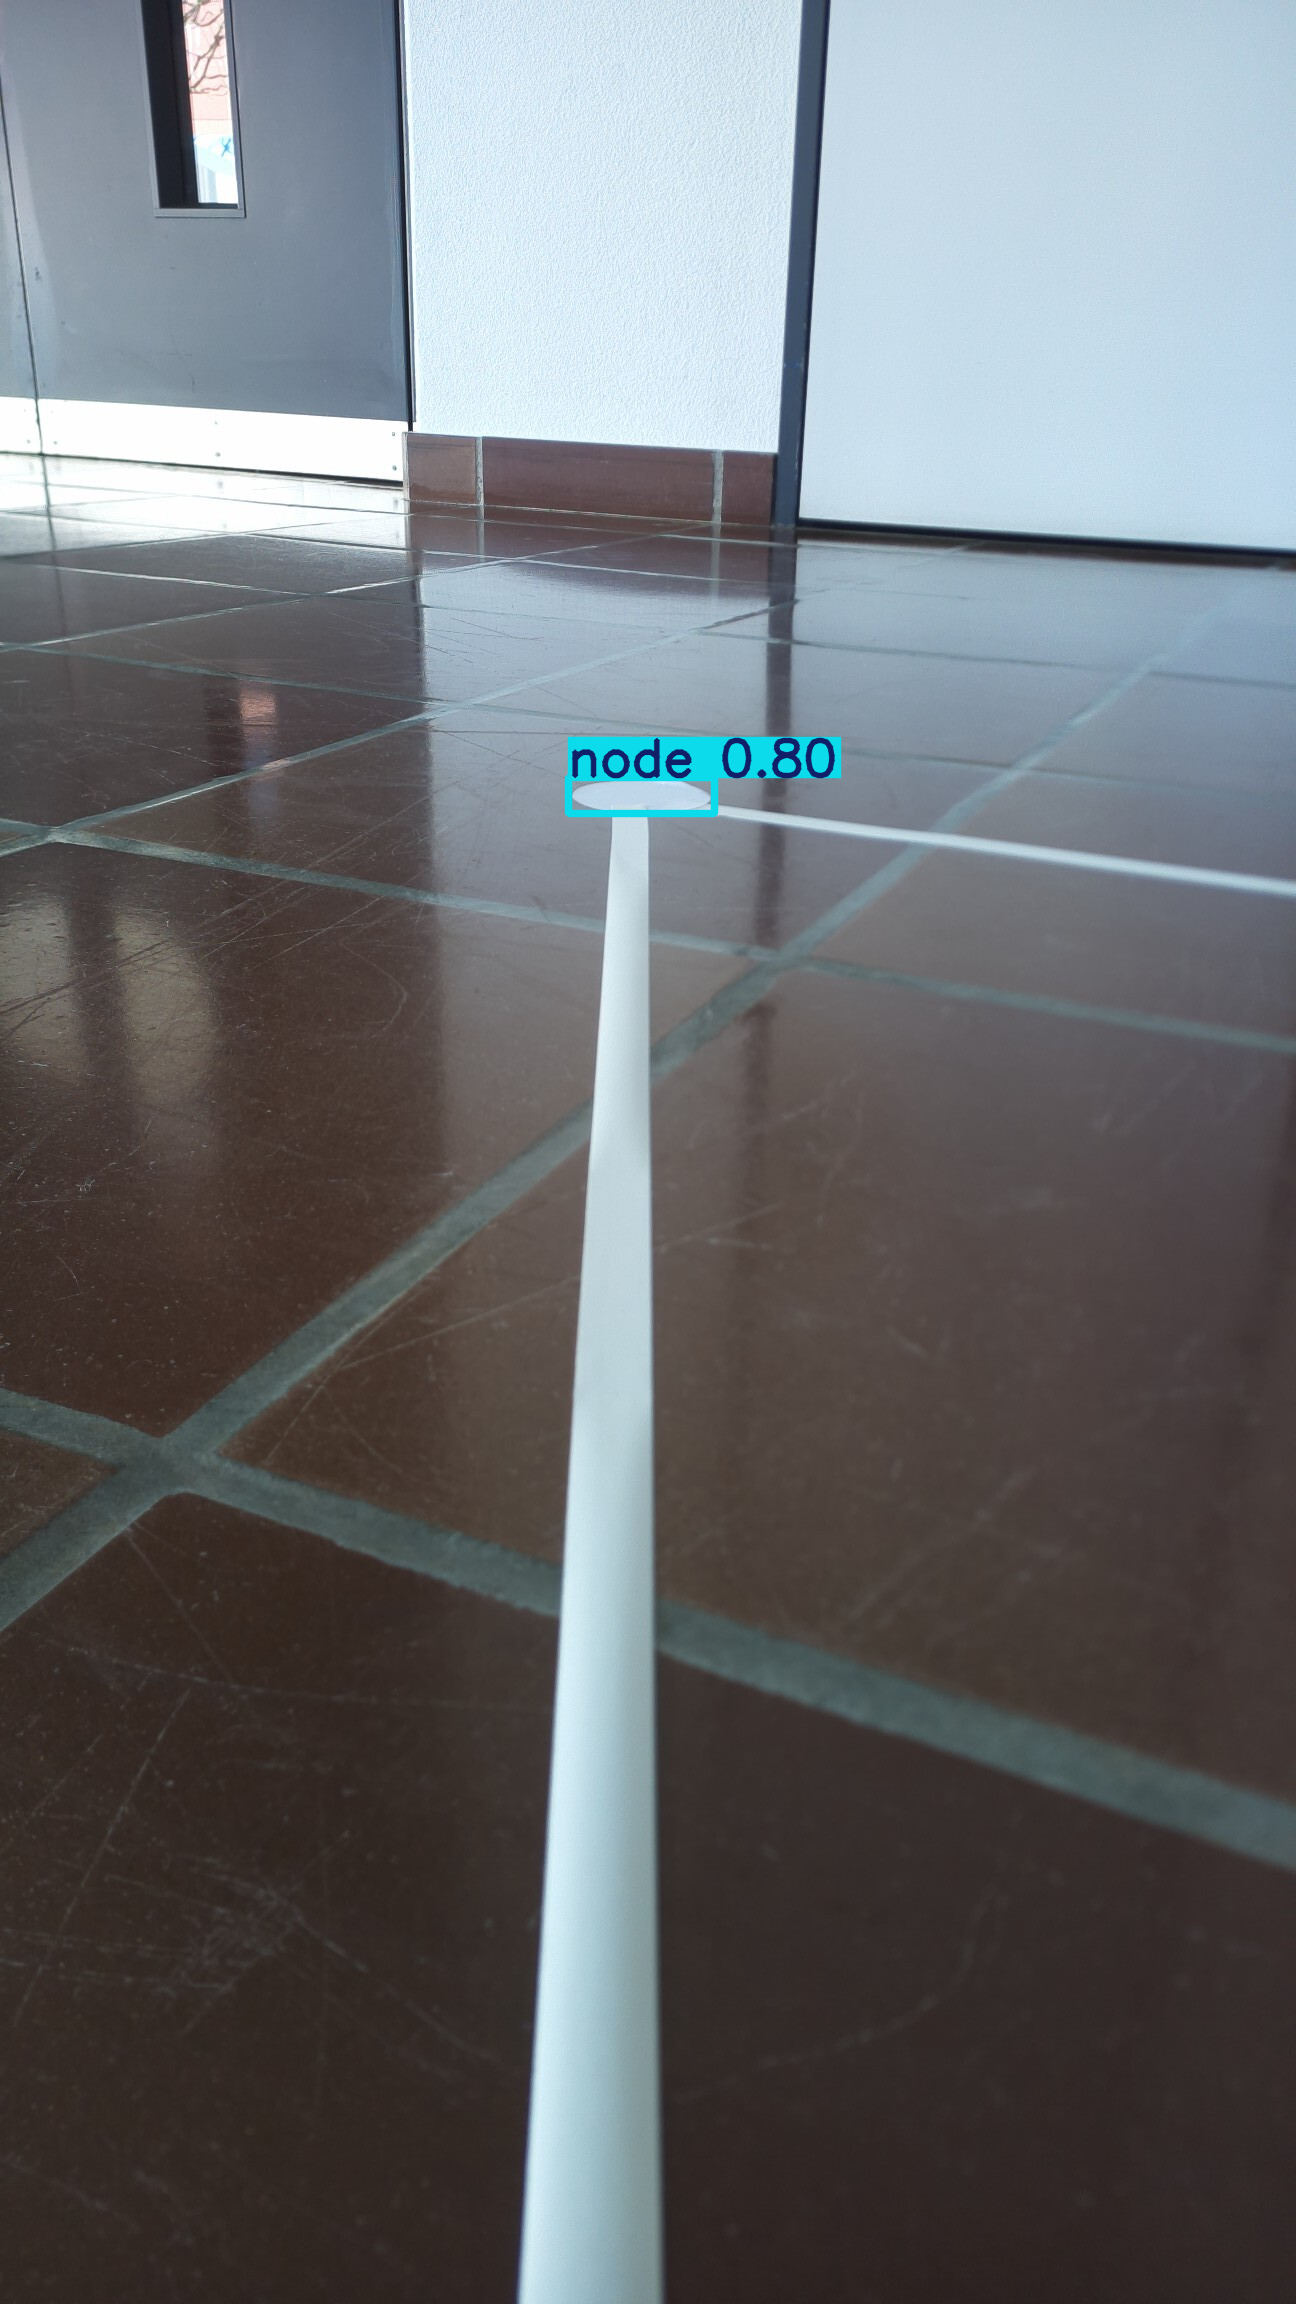
\includegraphics[width=\textwidth]{assets/IT/testing/yolo/node_annot.png}
    \caption{Returned Knoten}
    \label{fig:expl-algo-2}
  \end{minipage}
    \hfill
  \begin{minipage}[b]{0.23\textwidth}
    \centering
    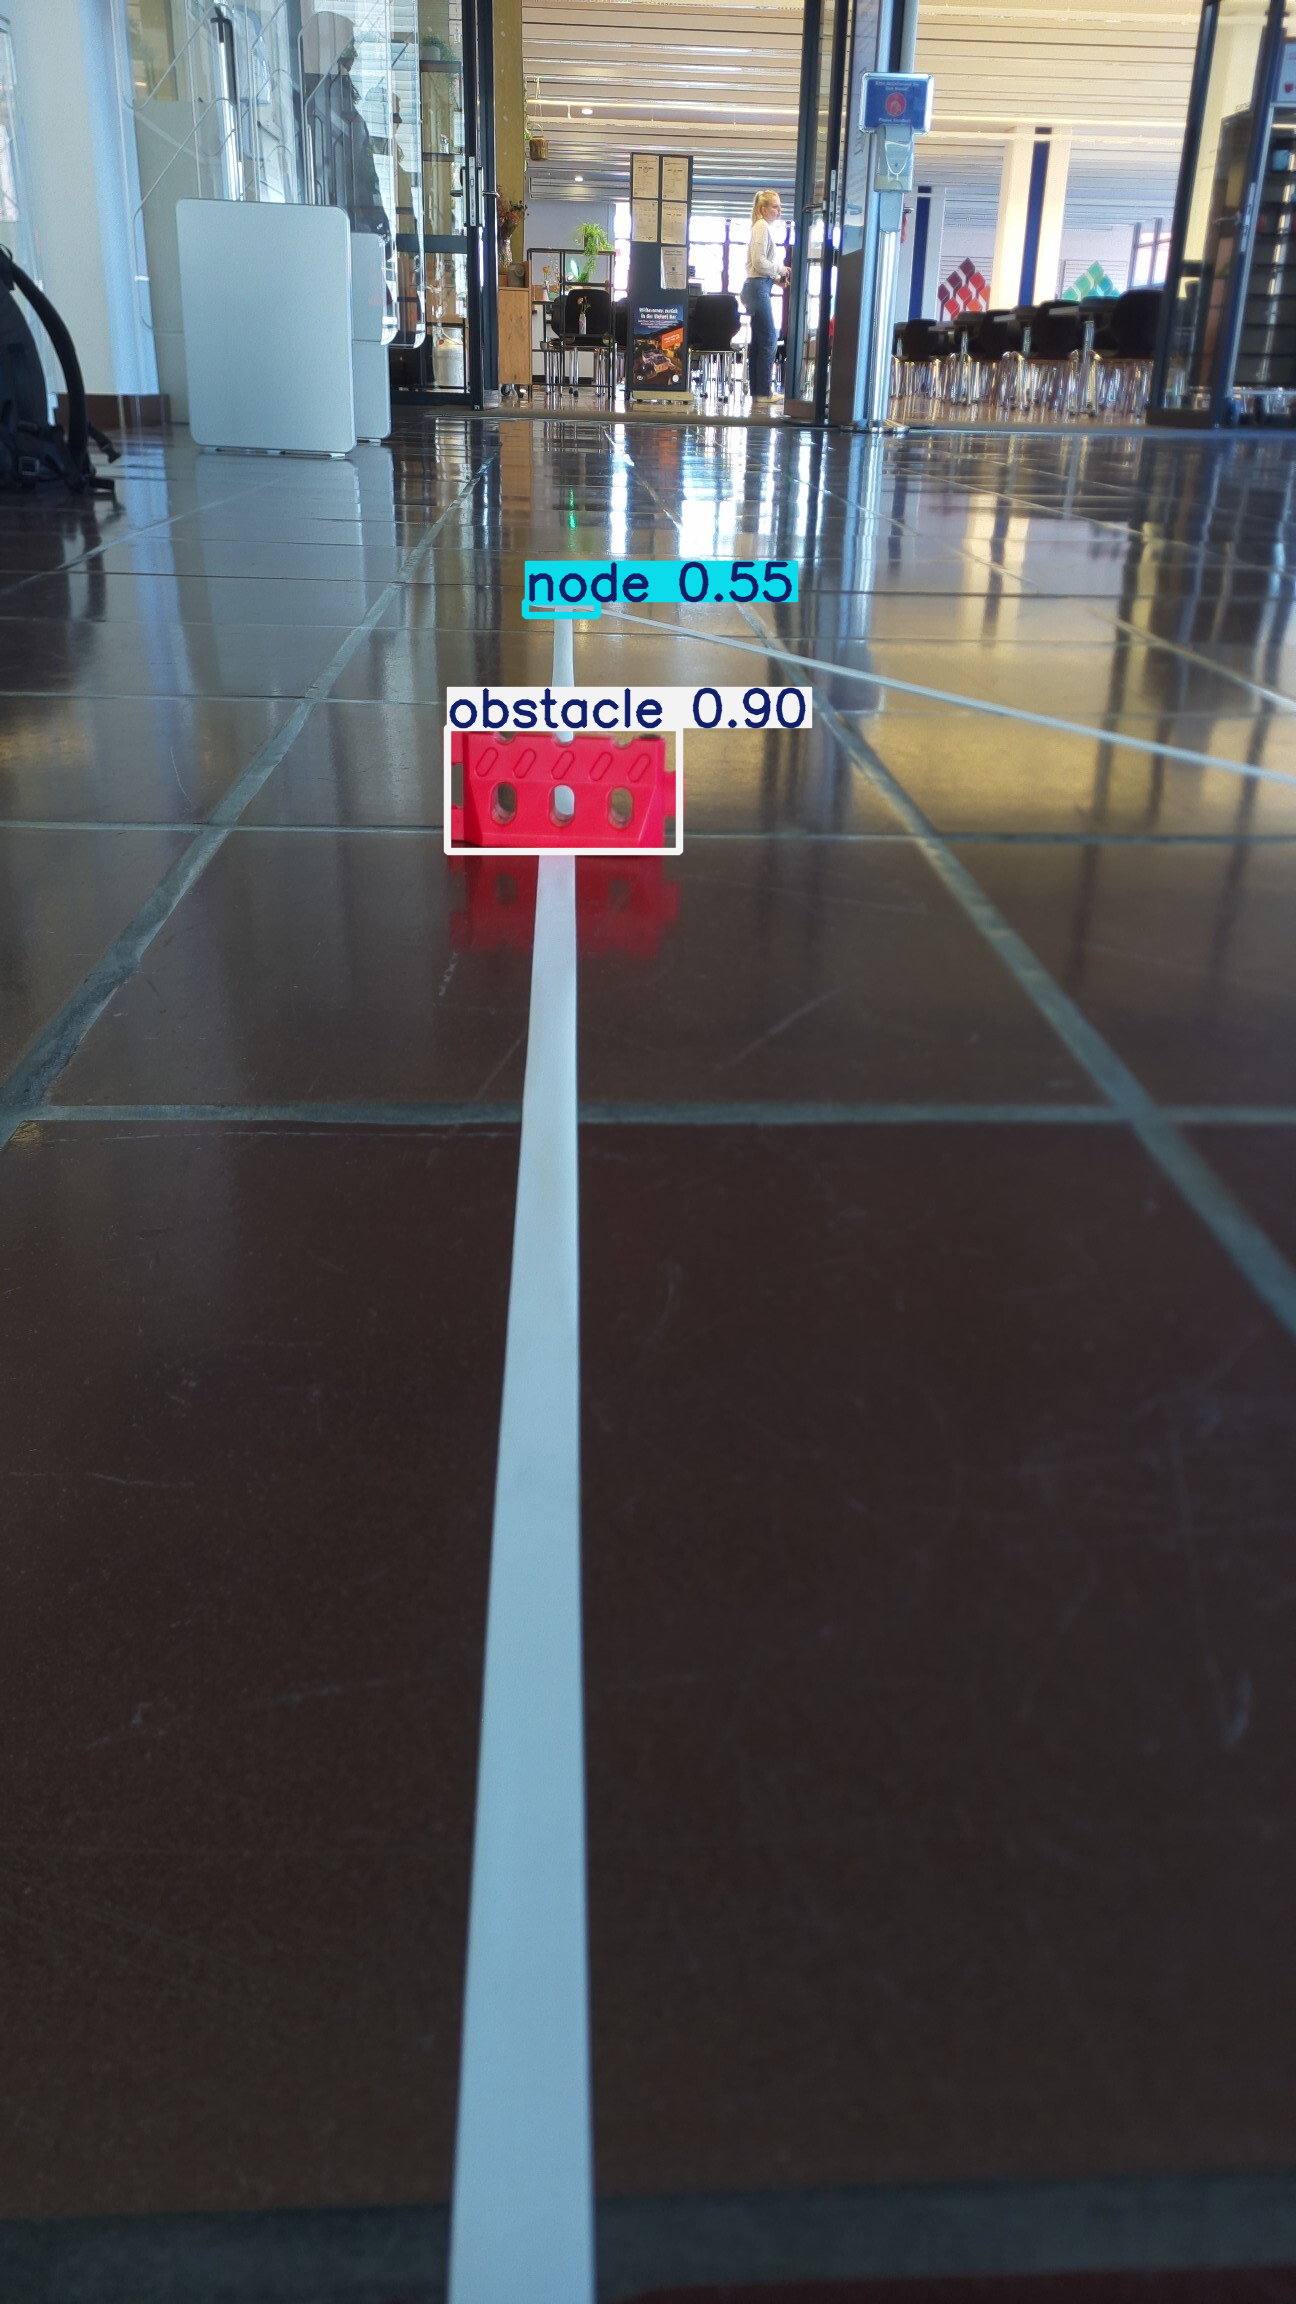
\includegraphics[width=\textwidth]{assets/IT/testing/yolo/barrier_annot.png}
    \caption{Returned Barriere}
    \label{fig:expl-algo-3}
  \end{minipage}
      \hfill
  \begin{minipage}[b]{0.23\textwidth}
    \centering
    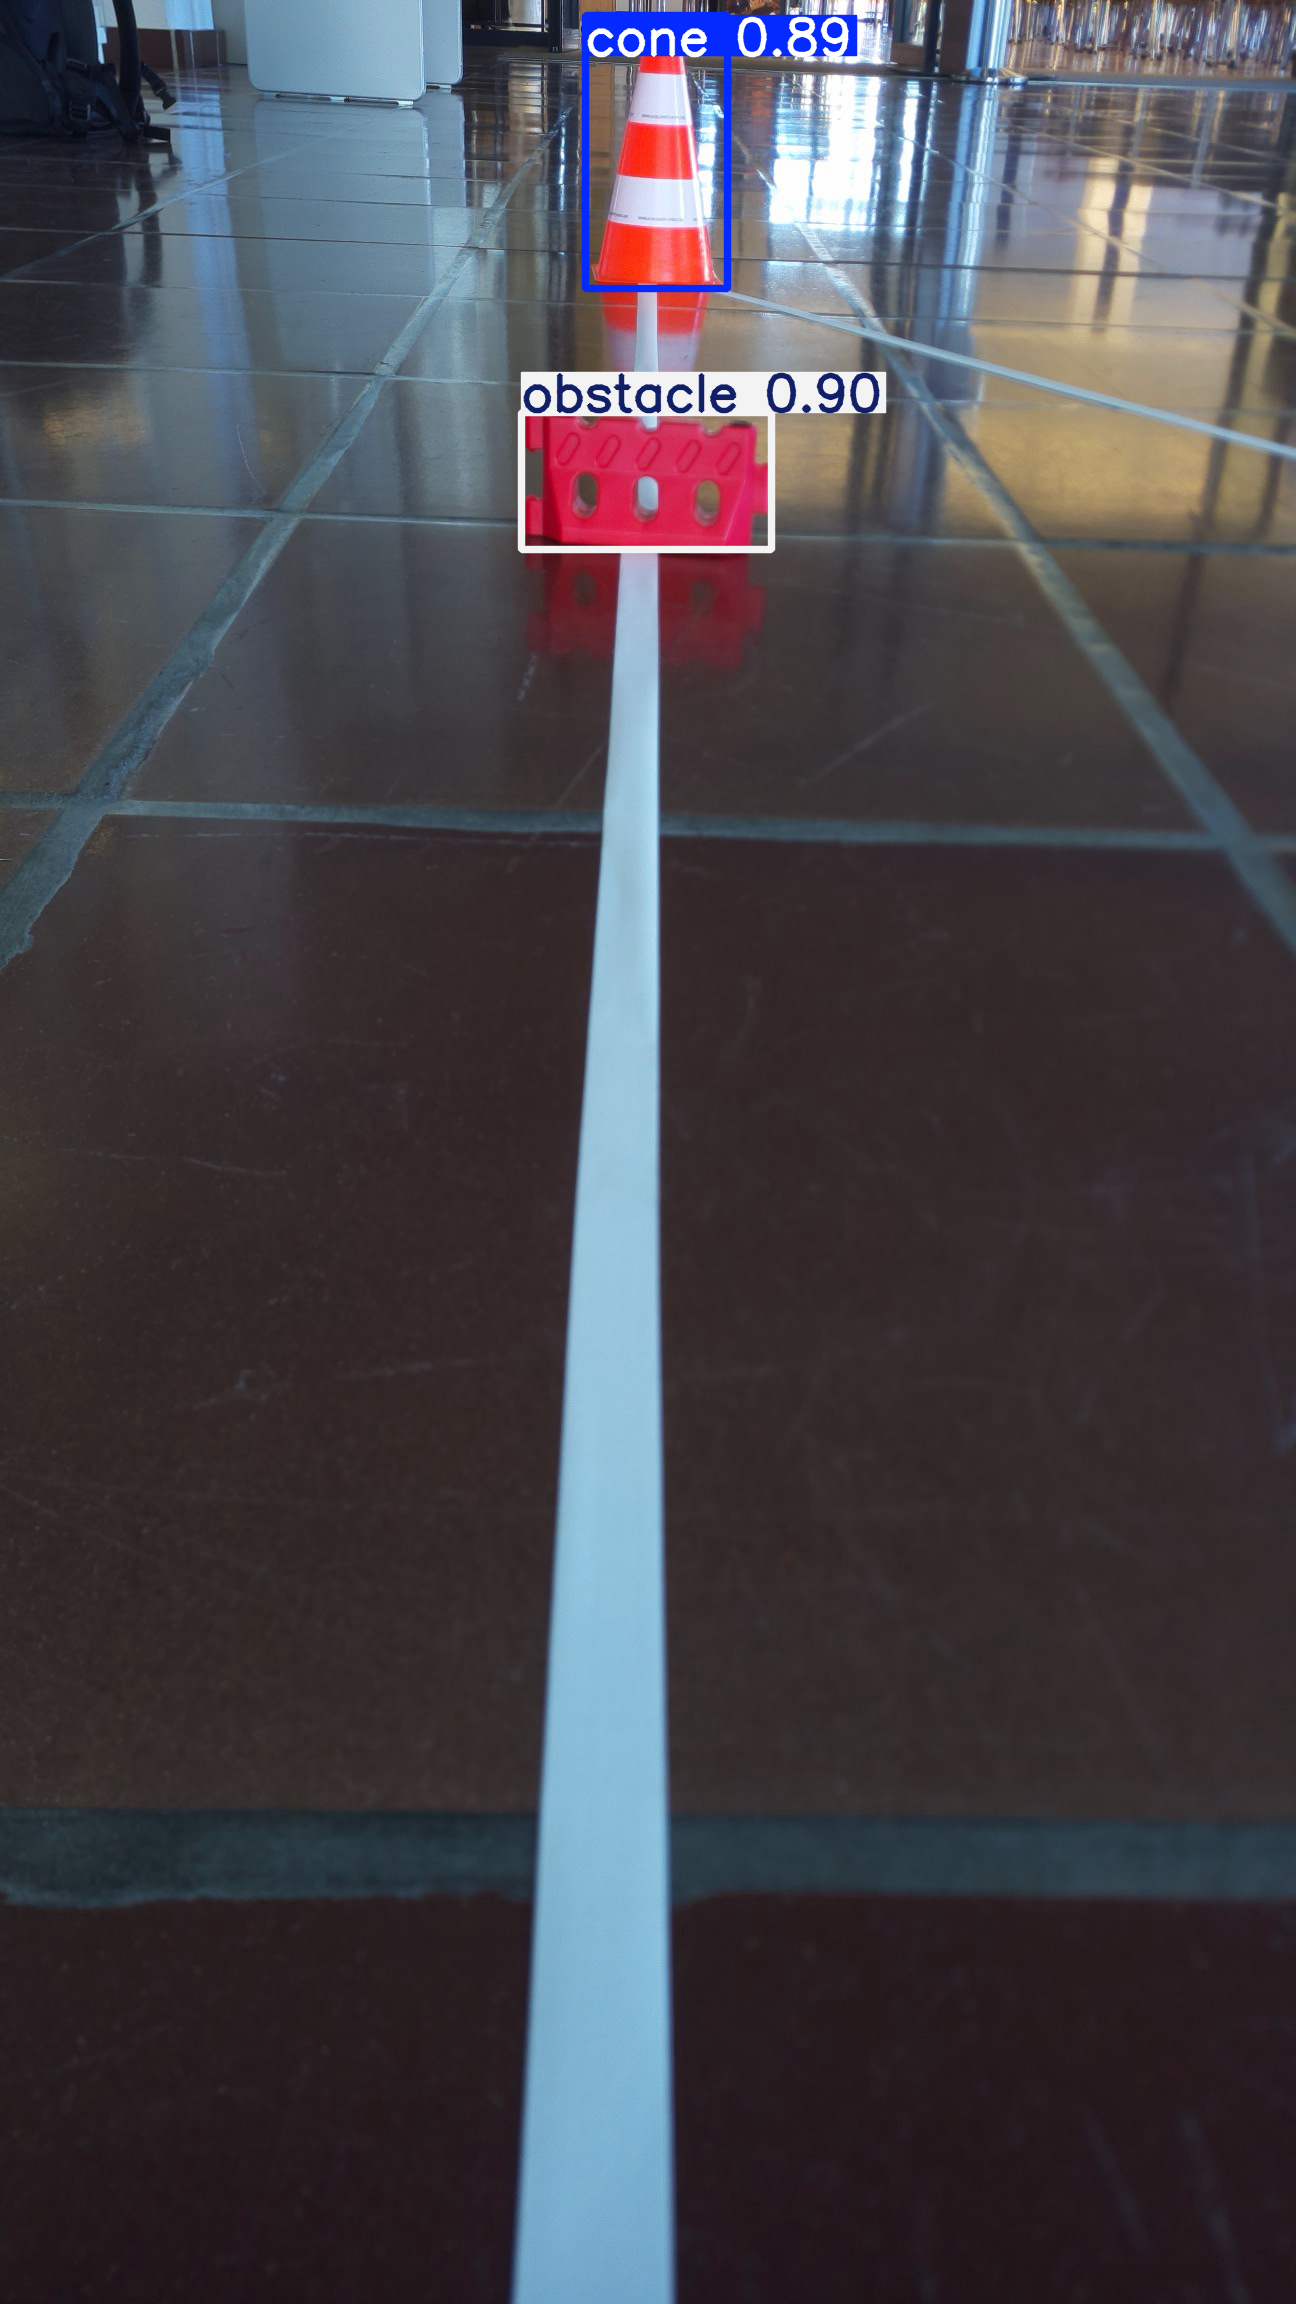
\includegraphics[width=\textwidth]{assets/IT/testing/yolo/pylon_behind_obst_annot.png}
    \caption{Returned Pylone}
    \label{fig:expl-algo-4}
  \end{minipage}
\end{figure}

Wie auf die einzelnen Objekte reagiert wird, ist in folgender Aufzählung beschrieben und ist gleich, wie in \acrshort{pren1} geplant.

\textbf{Pylonen erkennen}

Wird eine Pylone erkannt, wird der Knoten, der gerade geprüft wurde, inklusive alle Strecken dahin, aus dem internen Graphen entfernt.

\textbf{Knoten erkennen}

Wenn ein Knoten erkannt wird, dann geschieht nichts. Es wird interpretiert, dass sich kein Objekt auf diesem Weg befindet und die Strecke normal befahrbar ist.

\textbf{Barrieren erkennen}

Wird auf dem Bild eine Barriere erkannt, wird dies im internen Graphen gespeichert, indem die jeweilige Linie höher gewichtet wird, da es länger dauern wird diese zu überqueren.

\textbf{Entfernte Linien erkennen}

Die entfernten Linien werden erkannt, wenn die Winkel der ausgehenden Linien berechnet wird, Details dazu, gibt es in Kapitel \ref{outgoing-lines}. Die fehlende Linie wird aus dem internen Graphen entfernt.

\newpage
%%%%%%%%%%%%%%%%%Epic 11%%%%%%%%%%%%%%%%%%%%%%%%%%%%%%%%%%%%%%%%%%%%%%%%%%%%%%%
\subsection{Zieleingabe: Peripherie Ein- und Ausgabe}

In diesem Kapitel wird die Ein- und Ausgabe des Roboters thematisiert.
Dafür wurde auf dem Raspberry Pi ein Prototypen-HAT montiert, welcher die benötigten GPIO-Pins entsprechend der Abbildung \ref{fig:raspiheader-schema} auf Taster, Display und Buzzer verbindet.

\begin{figure}[H]
    \centering
    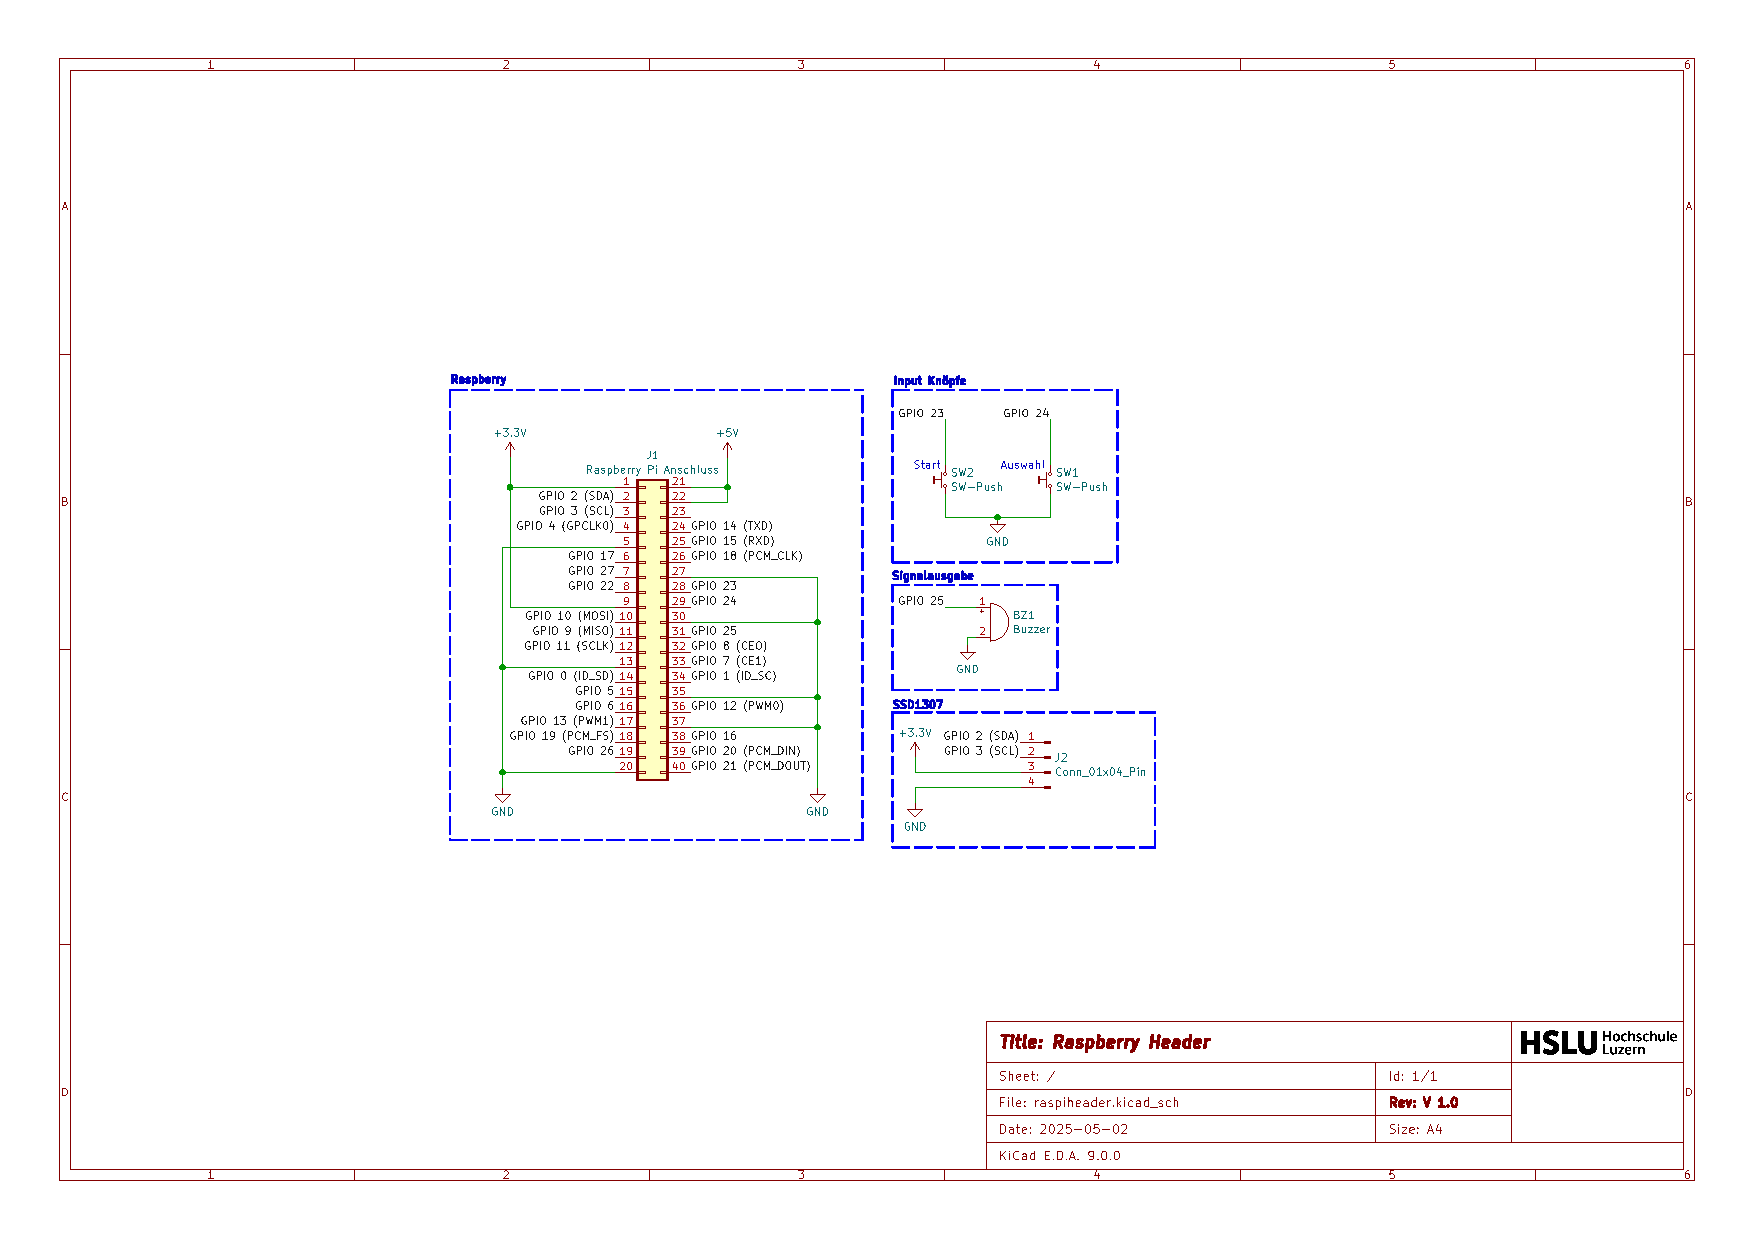
\includegraphics[width=\linewidth, trim=7.5cm 6cm 10cm 6cm, clip]{assets/ET/PCB/raspiheader.pdf}
    \caption{Raspberry Pi HAT Schema}
    \label{fig:raspiheader-schema}
\end{figure}

\begin{figure}[H]
    \centering
    \begin{subfigure}[t]{0.49\textwidth}
        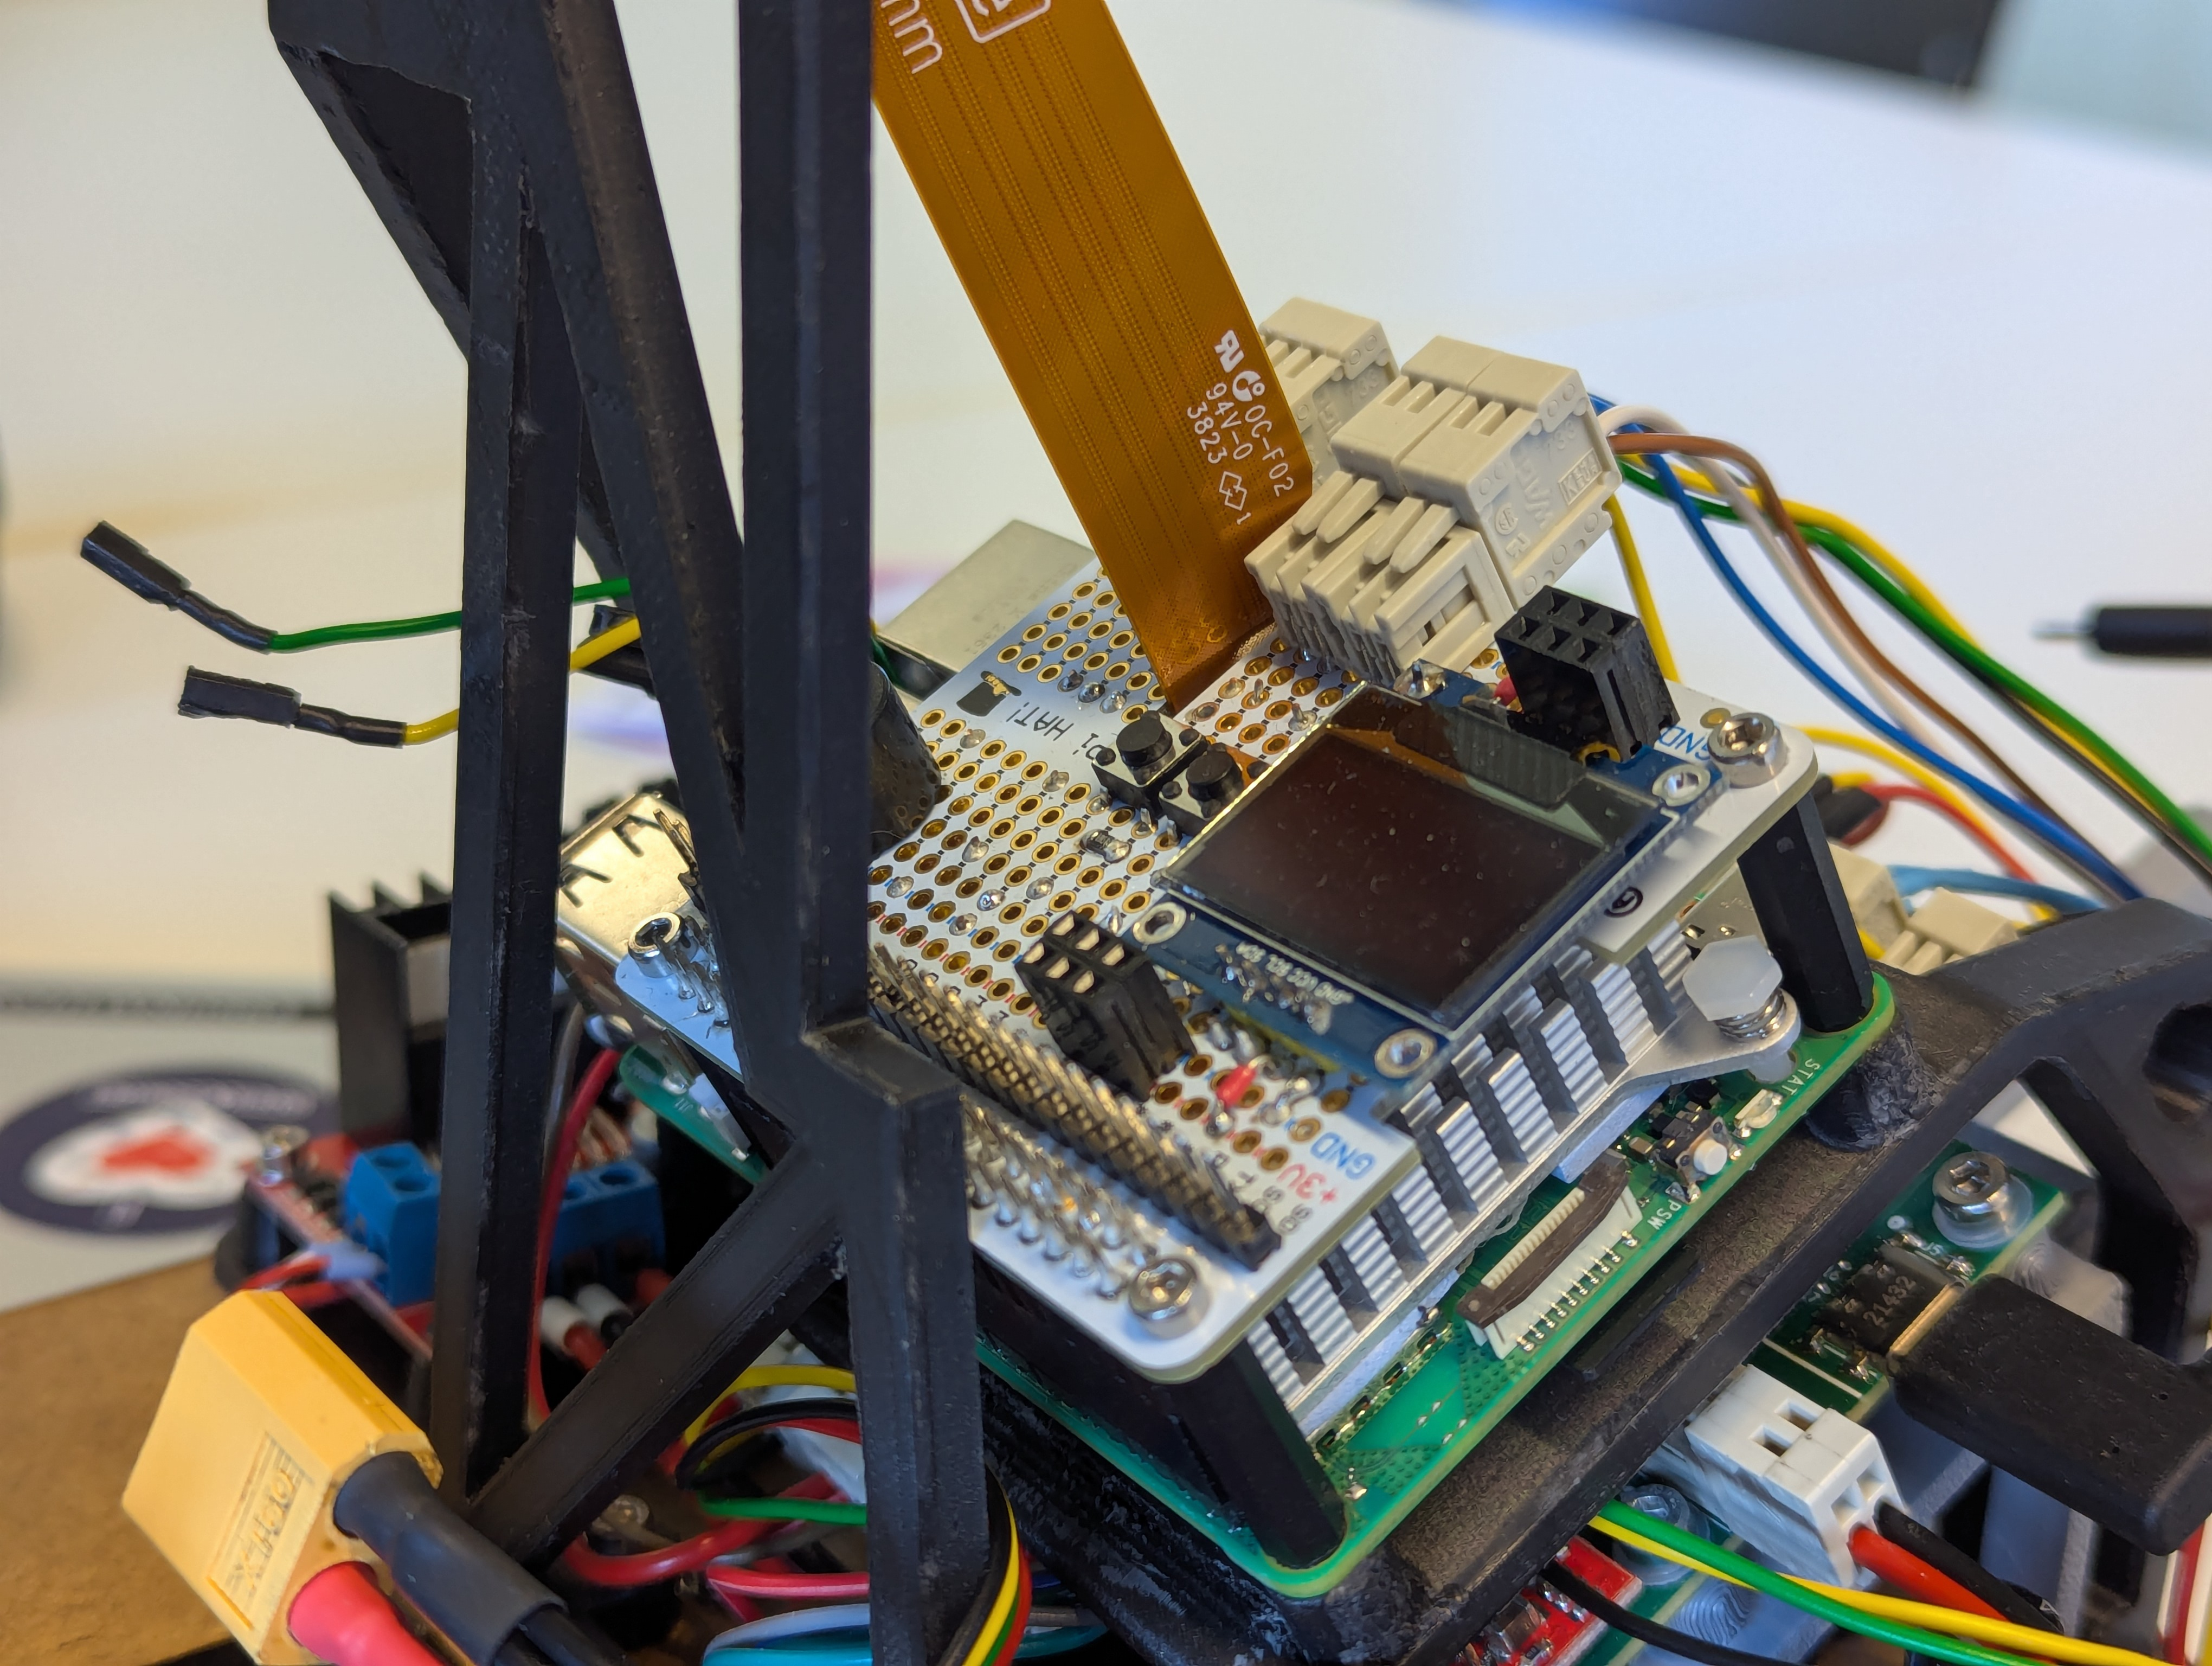
\includegraphics[width=\linewidth]{assets/IT/peripherie/raspi-hat_1.jpg}
    \end{subfigure}
    \hfill
    \begin{subfigure}[t]{0.49\textwidth}
        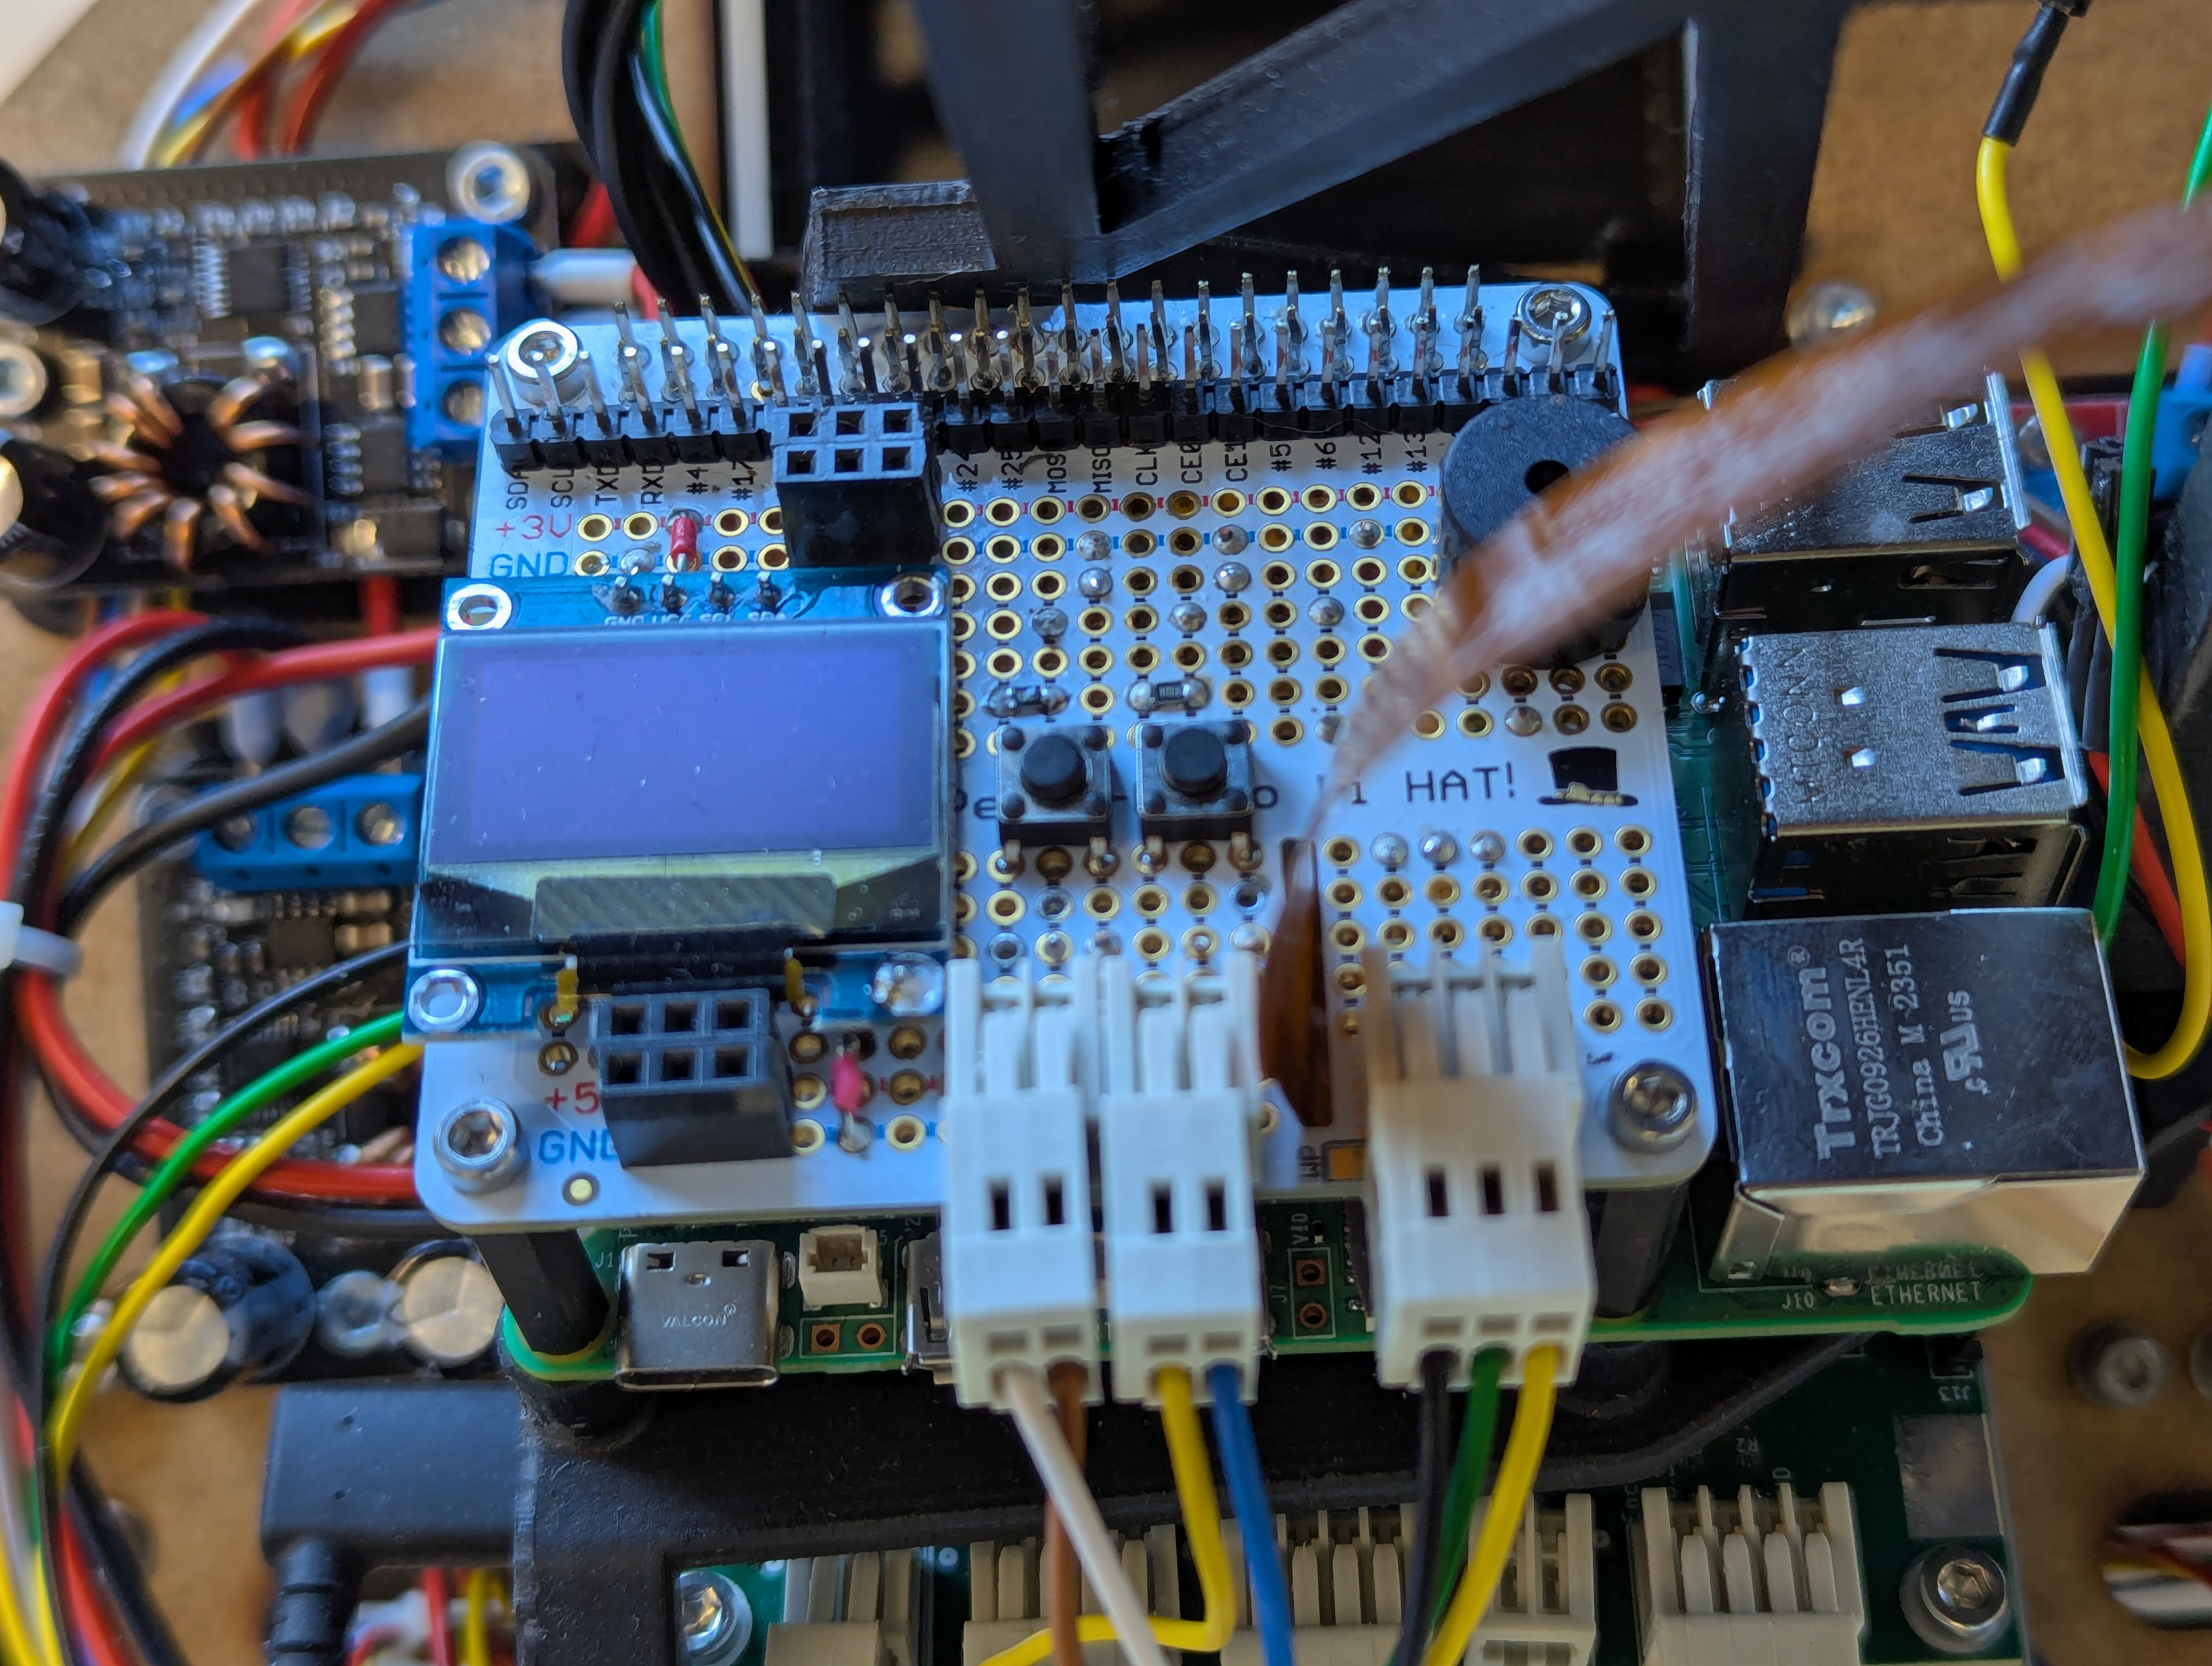
\includegraphics[width=\linewidth]{assets/IT/peripherie/raspi-hat_2.jpg}
    \end{subfigure}
    \caption{Raspberry Pi HAT zusammengebaut}
    \label{fig:raspiheader-assembly}
\end{figure}

Die Software dieser Komponenten wurde direkt in Python auf dem Raspberry Pi umgesetzt. Nachfolgend in Abbildung \ref{fig:peripherie-classdiagramm} ist das Klassendiagramm ersichtlich. Wir haben eine RealPeripherieConnector, welcher von BaseConnector erbt, und die Hardwarefunktionen wie Buttons und Buzzer übernimmt. Zusätzlich haben wir einen MockPeripherieConnector, welcher zum Einsatz kommt, wenn kein GPIO zur Verfügung steht. Dieser Simuliert die Ein und Ausgabe auf dem Terminal. Somit kann stets der Programmcode auf dem PC ausgeführt werden, wo keine, über GPIO verbundene, Buttons und Buzzers verfügbar sind.

\begin{figure}[H]
    \centering
    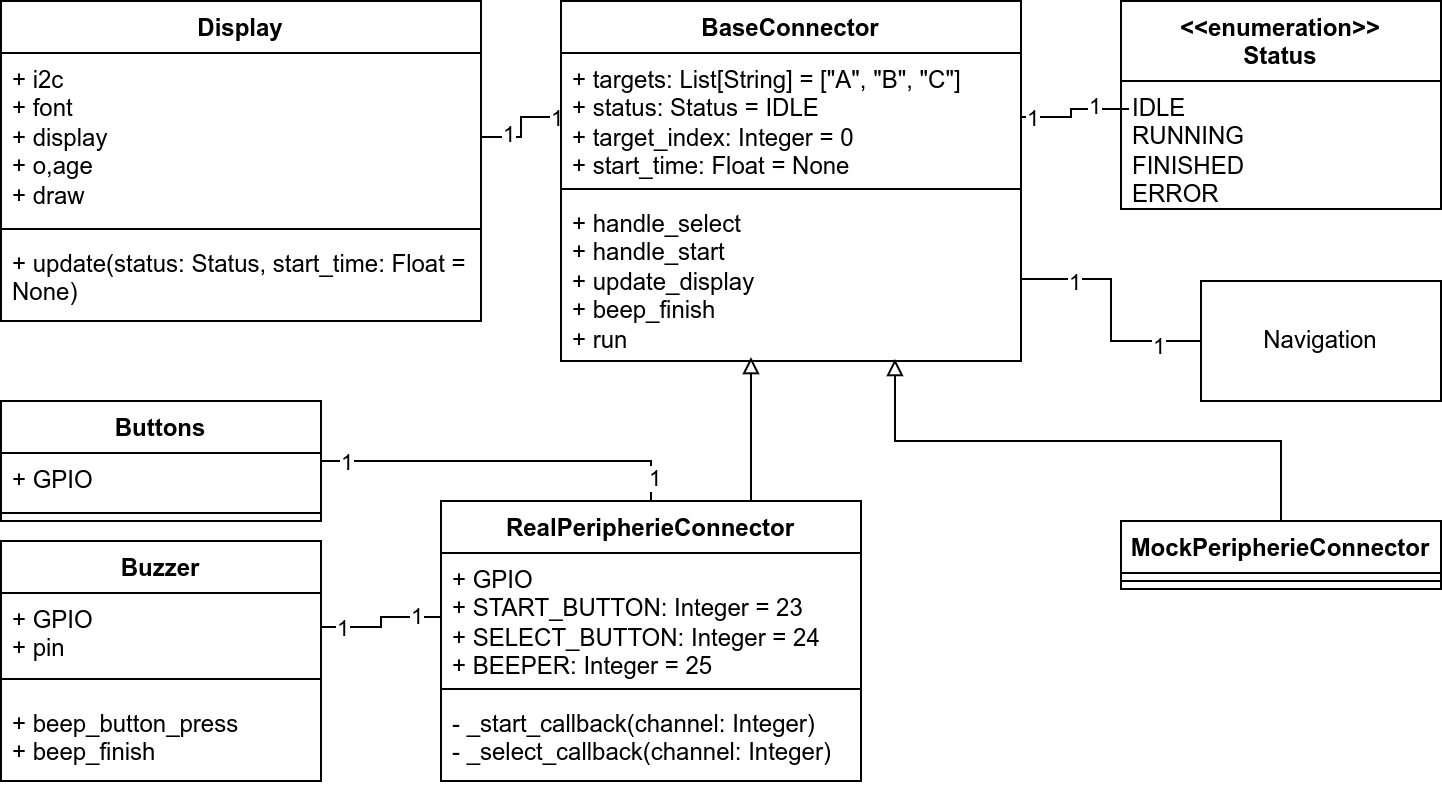
\includegraphics[width=\linewidth]{assets/IT/robot-sw-architecture-peripherie.png}
    \caption{Raspberry Pi HAT Klassendiagramm}
    \label{fig:peripherie-classdiagramm}
\end{figure}

\subsubsection{Peripherie Eingabe}
\label{zieleingabe}

\textbf{Zielknopf}

Die Zieleingabe wird dazu verwendet, um vor dem Start den geforderten Zielknoten auszuwählen. Bei Knopfdruck wird der gewählte Zielknoten durchgeschaltet, dies in der Reihenfolge A --> B --> C und dann wieder von vorne. So wird nur ein Taster benötigt, um zwischen den drei Zielen zu wechseln. Das Gewählte Ziel ist stets im Display (\ref{peripherie-display}) ersichtlich.

\textbf{Startknopf}

Der zweite Taster ist der Startknopf. Dieser wird nach der Eingabe des Zielknoten gedrückt, nach einer kurzen Wartezeit wird dann der Start initialisiert und der Roboter fängt an den Graphen Richtung Zielknoten zu traversieren.

Durch die einfache Zweitaster-Bedienung, und das ablesbare Display ist das Aufstellen sowie wählen des Zielknoten sehr gut unter 1 Minute möglich. 

\subsubsection{Peripherie Ausgabe}

\textbf{Display}\label{peripherie-display}

Das Display zeigt stets den aktuellen gewählten Zielknoten an, so kann einfach überprüft werden, welcher Zielknoten gewählt wird, bevor der Roboter gestartet wird. 
Zusätzlich wird der Status sowie die Laufzeit des Roboters dargestellt. Dadurch muss nicht separat eine Stoppuhr verwendet werden. Die Laufzeit wird automatisch beim erreichen des Zielknoten gestoppt und bleibt ablesbar.

TODO LUKAS: insert image of Display\\
TODO ALINA: Take image of each state of the display (IDLE, RUNNING, FINISHED)

\begin{figure}[H]
    \centering
    \begin{subfigure}[t]{0.30\textwidth}
        
\includegraphics[width=\linewidth]{assets/placeholder.png}
    \caption*{Status: IDLE}
    \end{subfigure}
    \hfill
    \begin{subfigure}[t]{0.30\textwidth}
        
\includegraphics[width=\linewidth]{assets/placeholder.png}
    \caption*{Status: RUNNING}
    \end{subfigure}
    \hfill
    \begin{subfigure}[t]{0.30\textwidth}
        
\includegraphics[width=\linewidth]{assets/placeholder.png}
    \caption*{Status: FINISHED}
    \end{subfigure}
    \caption{Raspberry Pi Display}
    \label{fig:raspiheader-display}
\end{figure}


\textbf{Buzzer}\label{peripherie-buzzer}

Der Buzzer ertönt sobald der Zielknoten erreicht wurde. Somit wird dem Bediener und Publikum vermittelt, dass der Roboter seine Traversierung beendet hat, und sich am Zielknoten befindet.

    %%%%%%%%%%%%%%%%%Epic 12%%%%%%%%%%%%%%%%%%%%%%%%%%%%%%%%%%%%%%%%%%%%%%%%%%%%%%%
\subsection{Ziel erreichen}

Es ist gefordert, dass der Roboter weiss, dass er sich im Ziel befindet und dies erkenntlich gibt mit einem Buzzer Geräusch, welches schon im vorangegangenen Kapitel \ref{peripherie-buzzer} beschrieben ist.

\subsubsection{Zielknoten erkennen}
\label{detect-target}

Es wurde bereits in \acrshort{pren1} die Methode gewählt, mit welcher die Buchstaben auf den Zielknoten erkannt werden sollen. Dieser Code muss nun lediglich migriert werden, um in die Architektur der Navigation zu passen.

Wie geplant wird der \gls{orb-gloss} Algorithmus verwendet, der in der OpenCV Library vorhanden ist. Es wird die TargetNodeReader Klasse im NodeReader Modul erstellt (siehe Abbildung \ref{fig:nav-arch}). Sobald eine Instanz dieser Klasse erstellt wird, lernt sie die Konturen von den Buchstaben A, B und C und speichert diese .
Dies lernt sie von den Beispielbildern von schwarzen Buchstaben auf weissem Hintergrund.
Jedes Mal wenn der Roboter einen Knoten fotografiert, wird dieses Bild verzerrt, um den Knoten in Vogelperspektive anzuzeigen (siehe Kapitel \ref{outgoing-lines}) und dann wird detektiert, ob sich darauf der Buchstabe des Zielknotens befindet. Falls der Zielknoten sich darauf befindet, macht der Roboter ein Buzzergeräusch (siehe Kapitel \ref{peripherie-buzzer}).

Auf folgender Grafik ist die Klasse in Verhältnis zu dem Navigator dargestellt.

\begin{figure}[H]
\centering
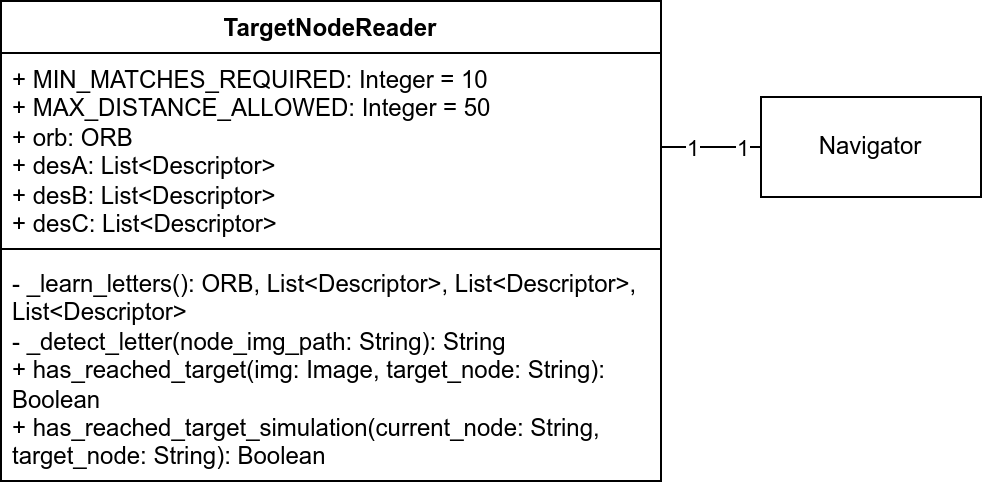
\includegraphics[width=\textwidth]{assets/IT/robot-sw-architecture-target-node-detector.png}
\caption{TargetNodeDetector Klassendiagramm}
\label{fig:target-node-nav}
\end{figure}

\acrshort{orb} gibt jeweils zurück, wie nahe die Anhaltspunkte des richtigen Objektes den Beispielbildern, die er gelernt hat, ist. Damit die Navigation in der Lage ist sowohl den richtigen Buchstaben zu erkennen, als auch jegliche Absenz eines Buchstabens, muss definiert werden, wie sicher sich der Algorithmus sein muss, dass es sich um einen Buchstaben handelt, damit es akzeptiert wird. Dafür wurden die folgenden zwei Parameter definiert:
\begin{verbatim}
# Anzahl Anhaltspunkte die gefunden werden müssen
MIN_MATCHES_REQUIRED = 10
# Wie unterschiedlich die Anhaltspunkte sein dürfen,
# um immer noch als Match zu zählen
MAX_DISTANCE_ALLOWED = 50
\end{verbatim}

Eine genaue Erklärung dieser Parameter, sowie ein Protokoll, wie die Werte ermittelt wurden, können im Anhang im Kapitel \nameref{target-node-unittests} gefunden werden.

Diese Funktionalität wurde erneut mit Unittests getestet.
Dabei wird die Klasse, welche die Konturen der Buchstaben lernt, instanziert und es werden realistische Bilder an die Methode übergeben, welche die Knoten liest. Alle Buchstaben inklusive Knoten ohne Buchstaben werden richtig erkannt. Diese Tests sind ebenfalls im Anhang im Kapitel \nameref{target-node-unittests} zu finden.

Durch die ausführlichen Tests kann das Risiko 22, dass der Roboter das Ziel verpasst oder es sich eingebildet, sehr stark mitigiert werden (siehe Tabelle \ref{table:risks}).

Damit die Navigation nach wie vor auf allen Umgebungen laufen kann, werden hier zwei Methoden erstellt. Eine Dummy Methode, die aus dem Simulator übernommen wurde und die richtige Methode, die Buchstaben von Bildern detektiert. Auf diese Weise kann einfach hin und her gewechselt werden je nach Umgebung.


\newpage
%%%%%%%%%%%%%%%%%Epic 13%%%%%%%%%%%%%%%%%%%%%%%%%%%%%%%%%%%%%%%%%%%%%%%%%%%%%%%
\subsection{Funktion-Stop}


Der Hauptschalter ist leicht zugänglich vorne am Roboter angebracht und trennt alle relevanten Funktionen vom Stromkreis. Befindet sich der Schalter in der unteren Stellung (siehe Abbildung \ref{fig:Schaltergehäuse}), ist das Fahrzeug deaktiviert.
Eine Ausnahme bildet der Raspberry Pi, der auch bei deaktiviertem Hauptschalter weiterhin mit Strom versorgt wird. Dies ist bewusst so vorgesehen, um Datenverlust oder Dateisystemfehler durch unerwartetes Abschalten zu vermeiden.

Im Schemaauszug zur Verdrahtung des Hauptschalters ist ebenfalls ersichtlich, dass der Motortreiber Zugriff auf die Akkuspannung hat (siehe Abbildung \ref{fig: Verdrahtung Hauptschalter}). Dadurch können die Motoren mit einer höheren Spannung betrieben werden, was die Leistungsfähigkeit steigert. Zudem wurde darauf geachtet, dass die Masseverbindung zwischen dem Raspberry Pi und dem restlichen Fahrzeug ausschliesslich über die UART-Schnittstelle erfolgt. Auf diese Weise sollen unerwünschte Massepotenzialunterschiede und daraus resultierende Störströme vermieden werden.

\begin{figure}[H]
\centering
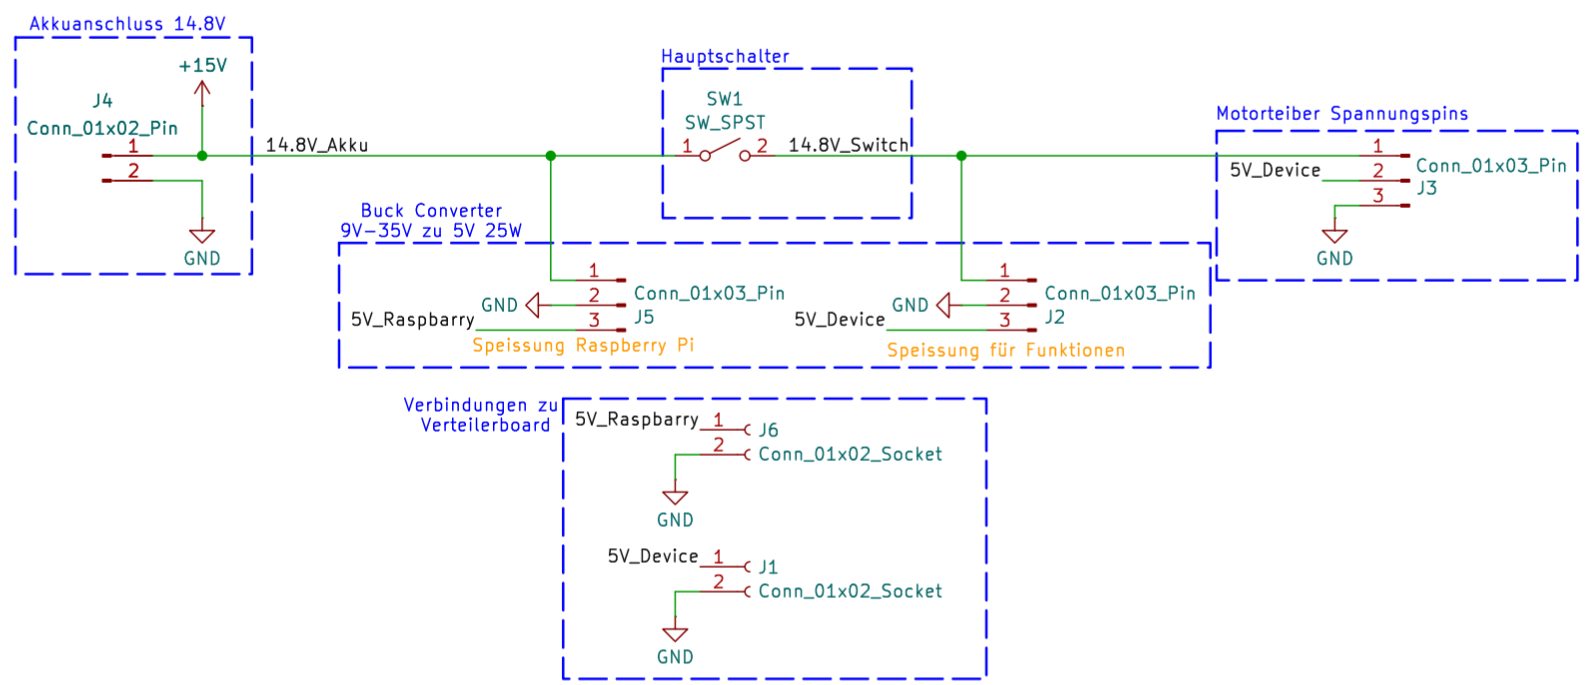
\includegraphics[width=\textwidth]{assets/ET/PINOUT/Speissung.png}
\caption{Verdrahtung Hauptschalter}
\label{fig: Verdrahtung Hauptschalter}
\end{figure}

\newpage
\subsubsection{Schaltergehäuse}

Am Schaltergehäuse werden der Hauptschalter und die zwei Inputtasten für die Zielauswahl und das Startsignal montiert. Das Gehäuse steht leicht erhöht auf Grundplatte. Unter dem Gehäuse werden die Kabel für den Ultraschallsensor durchgeführt.


\begin{figure}[H]
\centering
\includegraphics[width=0.5\textwidth, angle=-90, trim={10cm 0cm 10cm 0cm}, clip]{assets/MT/Schaltergehäuse.jpg}
\caption{Schaltergehäuse}
\label{fig:Schaltergehäuse}
\end{figure}


    \section{Realisiertes Funktionsmuster}

In diesem Kapitel wird die Umsetzung des in \acrshort{pren1} erarbeiteten Konzept anhand der erstellten Anforderungsliste (siehe Kapitel ``\nameref{anforderungliste}'') bewertet. Der Fokus liegt auf den Fest- und Mindestanforderungen.

\subsection{Anforderungen}

Die physischen Anforderungen an den Roboter konnten vollständig erfüllt werden. Das maximal zulässige Gewicht von 2 kg wurde mit einem Gesamtgewicht von 1.262 kg, insbesondere durch den Einsatz von Leichtbaustrukturen, deutlich unterschritten. Die maximale Baugrösse 300x300x800mm kann in der Startkonfiguration mit Greifer in Ausgangsstellung eingehalten werden. Zusätzlich erforderliche Komponenten wie ein Notausschalter, ein Eingabetaster zur Zieleingabe sowie eine Statusanzeige wurden erfolgreich integriert.

Der Roboter ist in der Lage eine bestimmte Distanz vor und zurück zu fahren und sich einen bestimmten Winkel zu drehen.

Durch diese Funktionen und den Greifer ist der Roboter in der Lage ein Hindernis mit einer Masse von 300g anzuheben und im Umkreis von 20mm am alten Ort abzusetzen. Auf Abbildungen \ref{fig:greifer-open} \& \ref{fig:griefe-rclose} ist das Greifen gezeigt.


\begin{figure}[H]
\centering
\begin{minipage}[b]{0.49\textwidth}
  \centering
    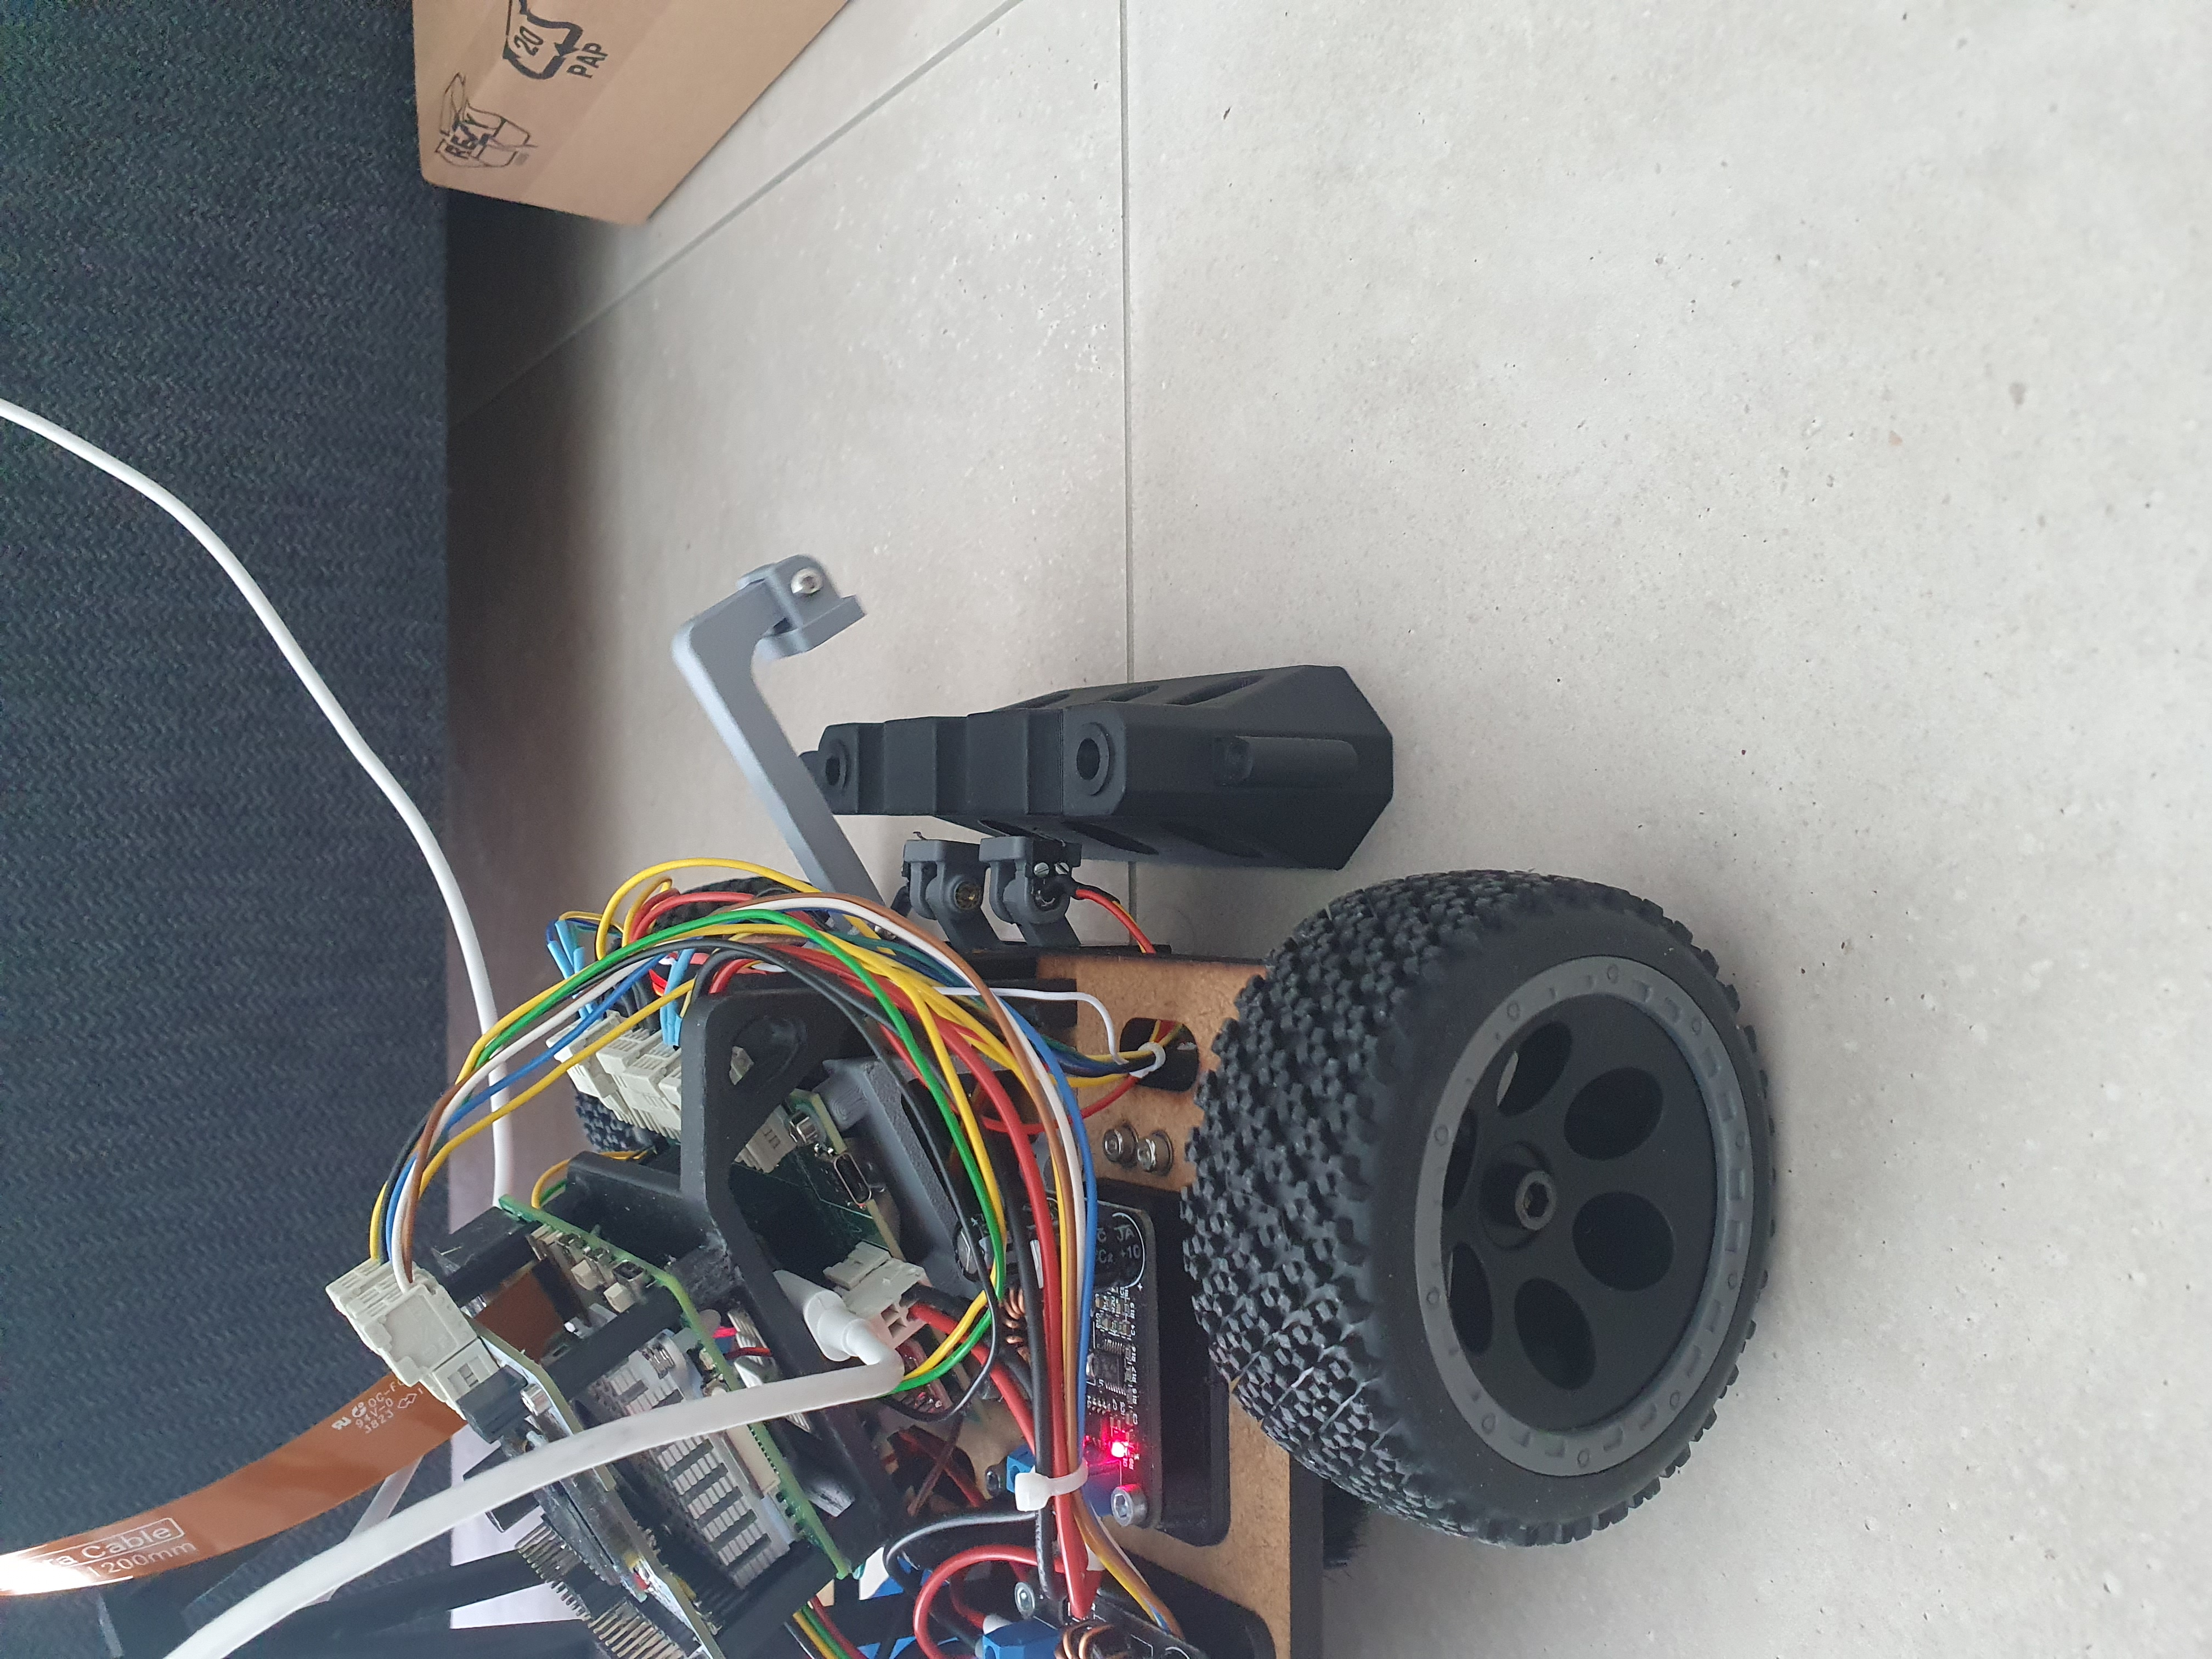
\includegraphics[width=\textwidth, angle=-90]{assets/MT/greifer-open.jpg}
    \caption{Greifer offen}
    \label{fig:greifer-open}
\end{minipage}
\hfill
\begin{minipage}[b]{0.49\textwidth}
  \centering
  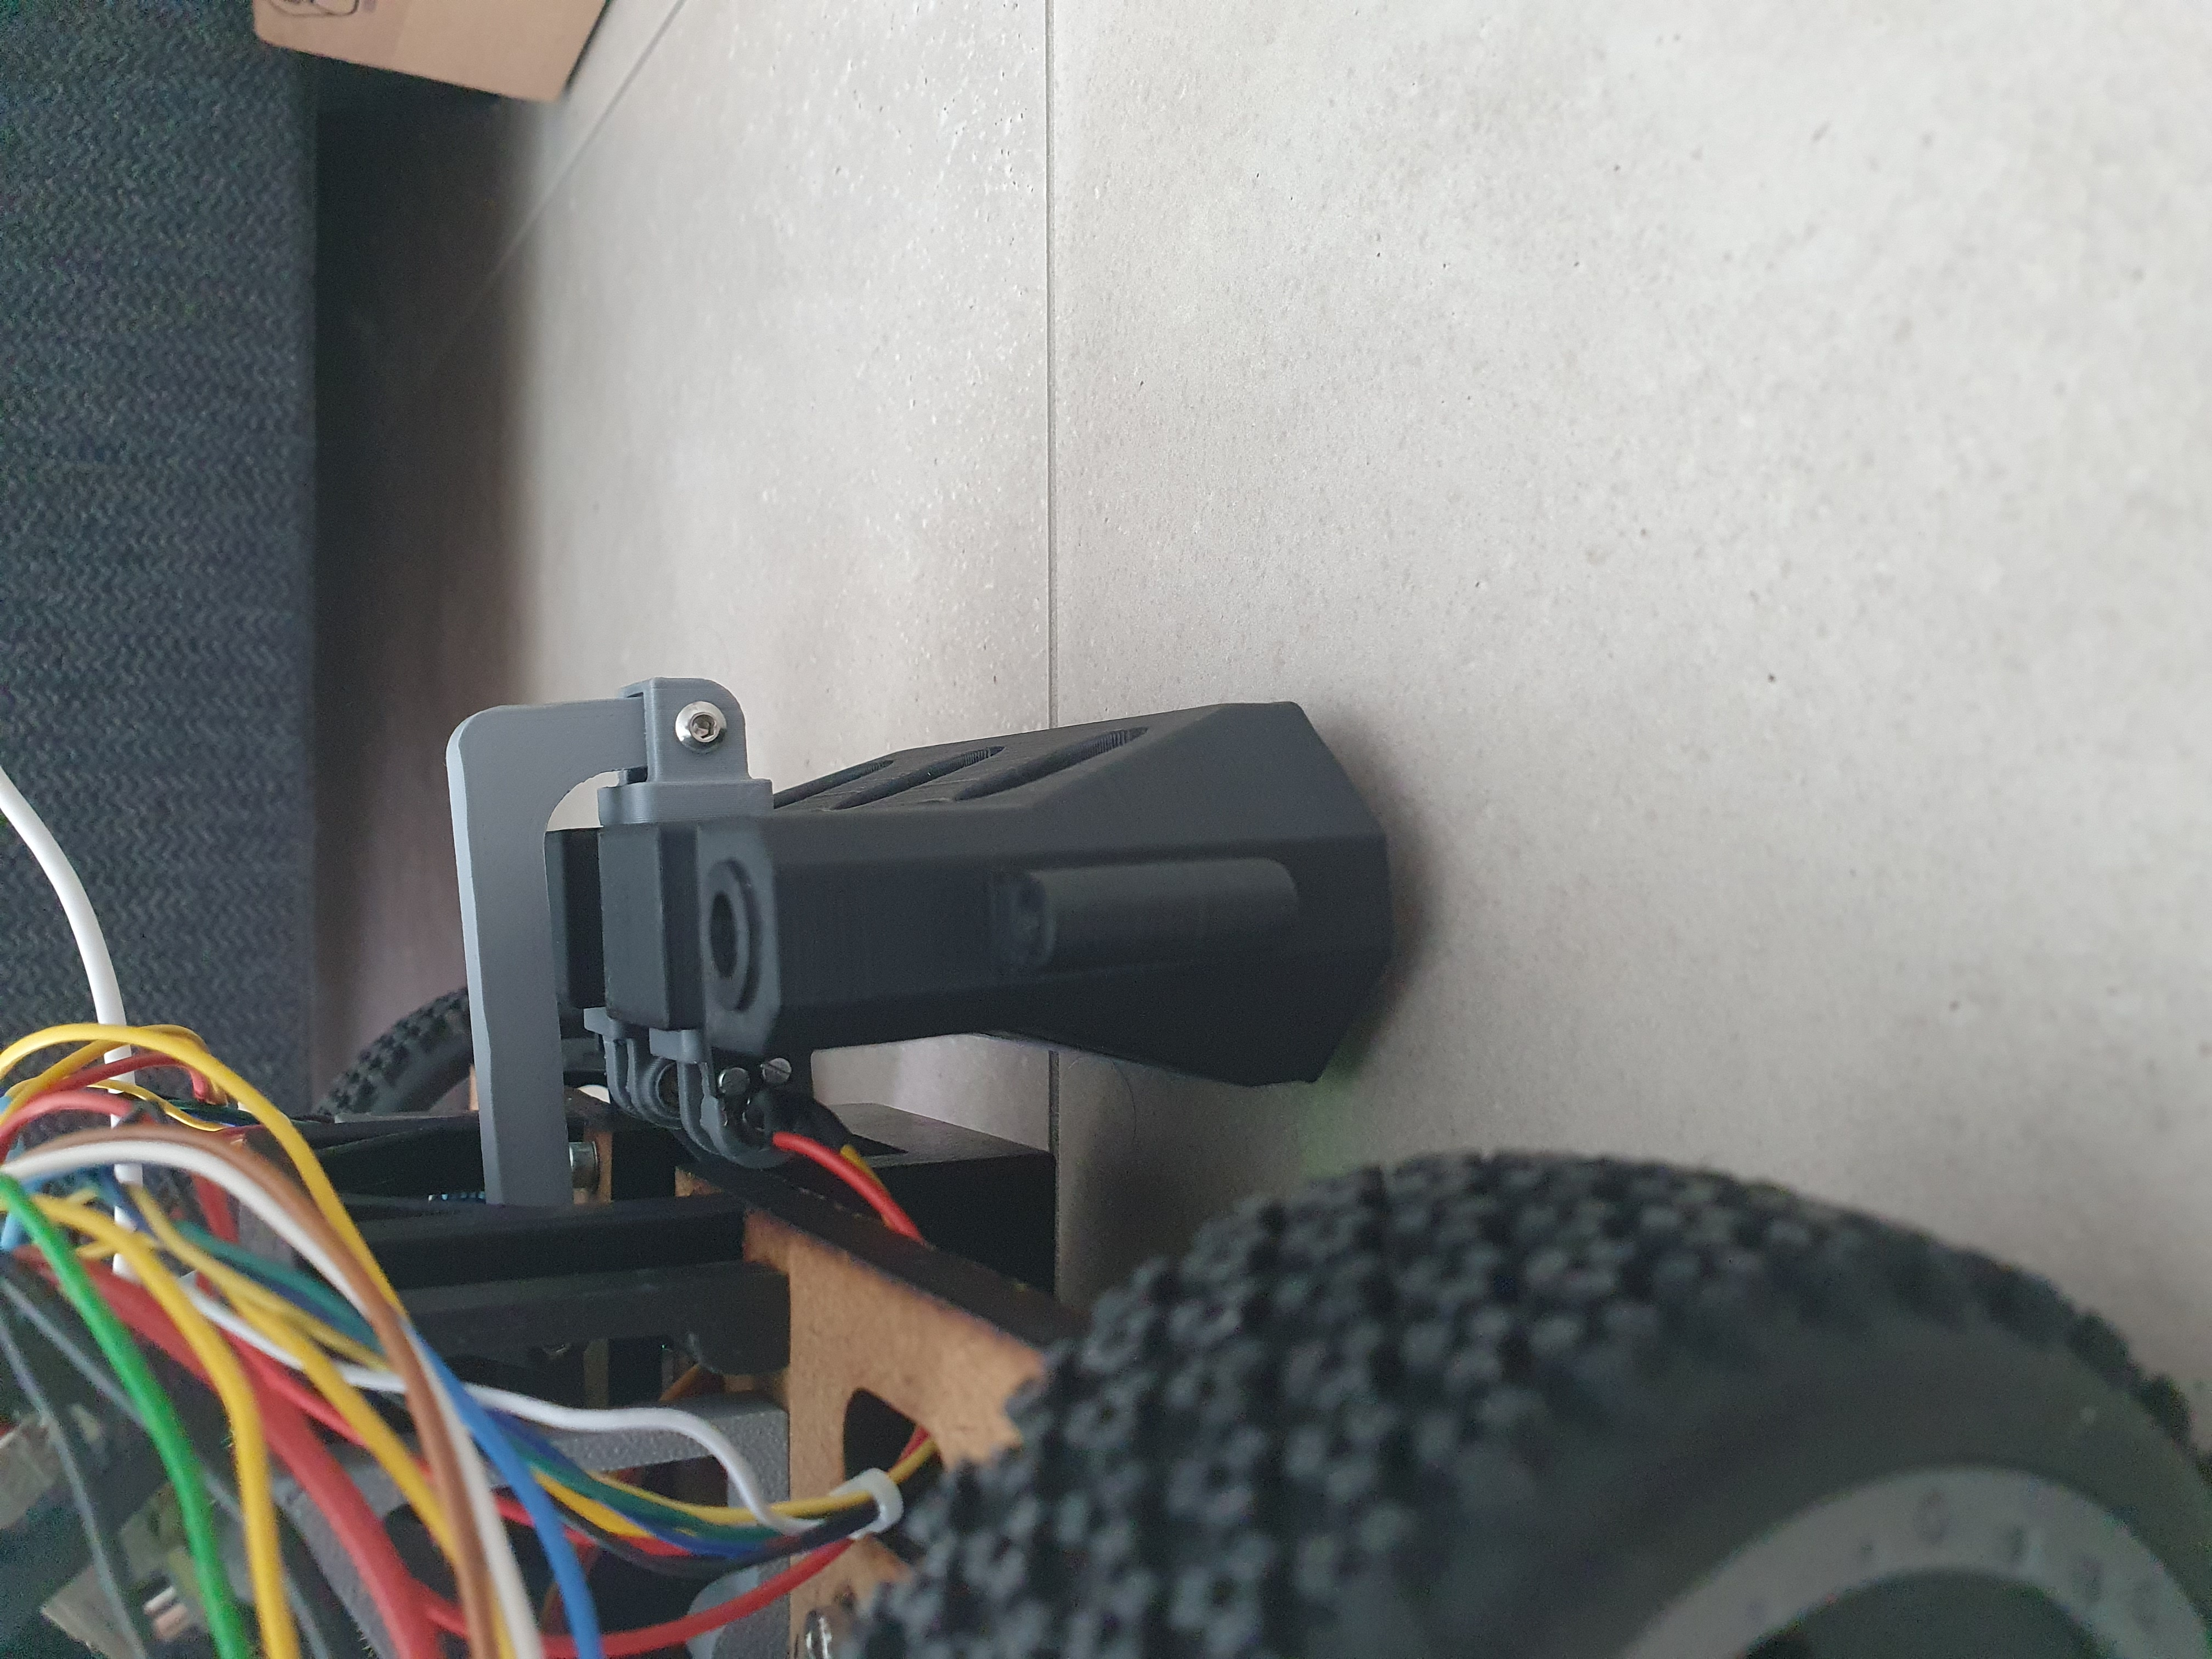
\includegraphics[width=\textwidth, angle=-90]{assets/MT/greifer-close.jpg}
  \caption{Greifer geschlossen}
  \label{fig:griefe-rclose}
\end{minipage}
\end{figure}

Das Folgen der Linie erfolgt wie in \acrshort{pren1} geplant mit einem Liniensensor, der aus mehreren Phototransistoren besteht. Die Regelung der Motoren erfolgt mit Hilfe eines PD-Reglers. Der PD-Regler konnte auf dem Testparcour geprüft werden und ist in der Lage der Linie zu folgen und auf einem Knoten anzuhalten.


% Used hyperlink beceause of includepdf instead of section to label
Die Bilderkennung und der Wegfindungsalgorithmus konnten mithilfe des Kameratestaufbaus aus \acrshort{pren1} und einem leicht veränderten Code bereits vor Ort getestet werden (siehe Anhang \hyperlink{statische-traver.1}{Testprotokoll Statische Traversierung}). Gesperrte Knoten konnten bei den Testläufen mit einer 100\% Sicherheit erkennt werden, ebenso konnten die Barrieren in 100\% der Fälle erkannt werden. Dies bezieht sich auf die manuellen Testdurchläufe und das Trainingsresultat des Models (siehe Confusion Matrix auf Abbildung \ref{fig:conf-matrix-model}. Trotzdem wird mit dem Ultraschall eine zusätzliche Sicherung eingebaut. Dieser misst auf \pm 1cm zuverlässig, wie nahe sich ein Objekt vor dem Roboter befindet.

Auch die Erkennung der ausgehenden Kanten war immer erfolgreich. Der Algorithmus hat bei allen Testdurchläufen einen direkten Weg ins Ziel gefunden. 

\begin{figure}[H]
\centering
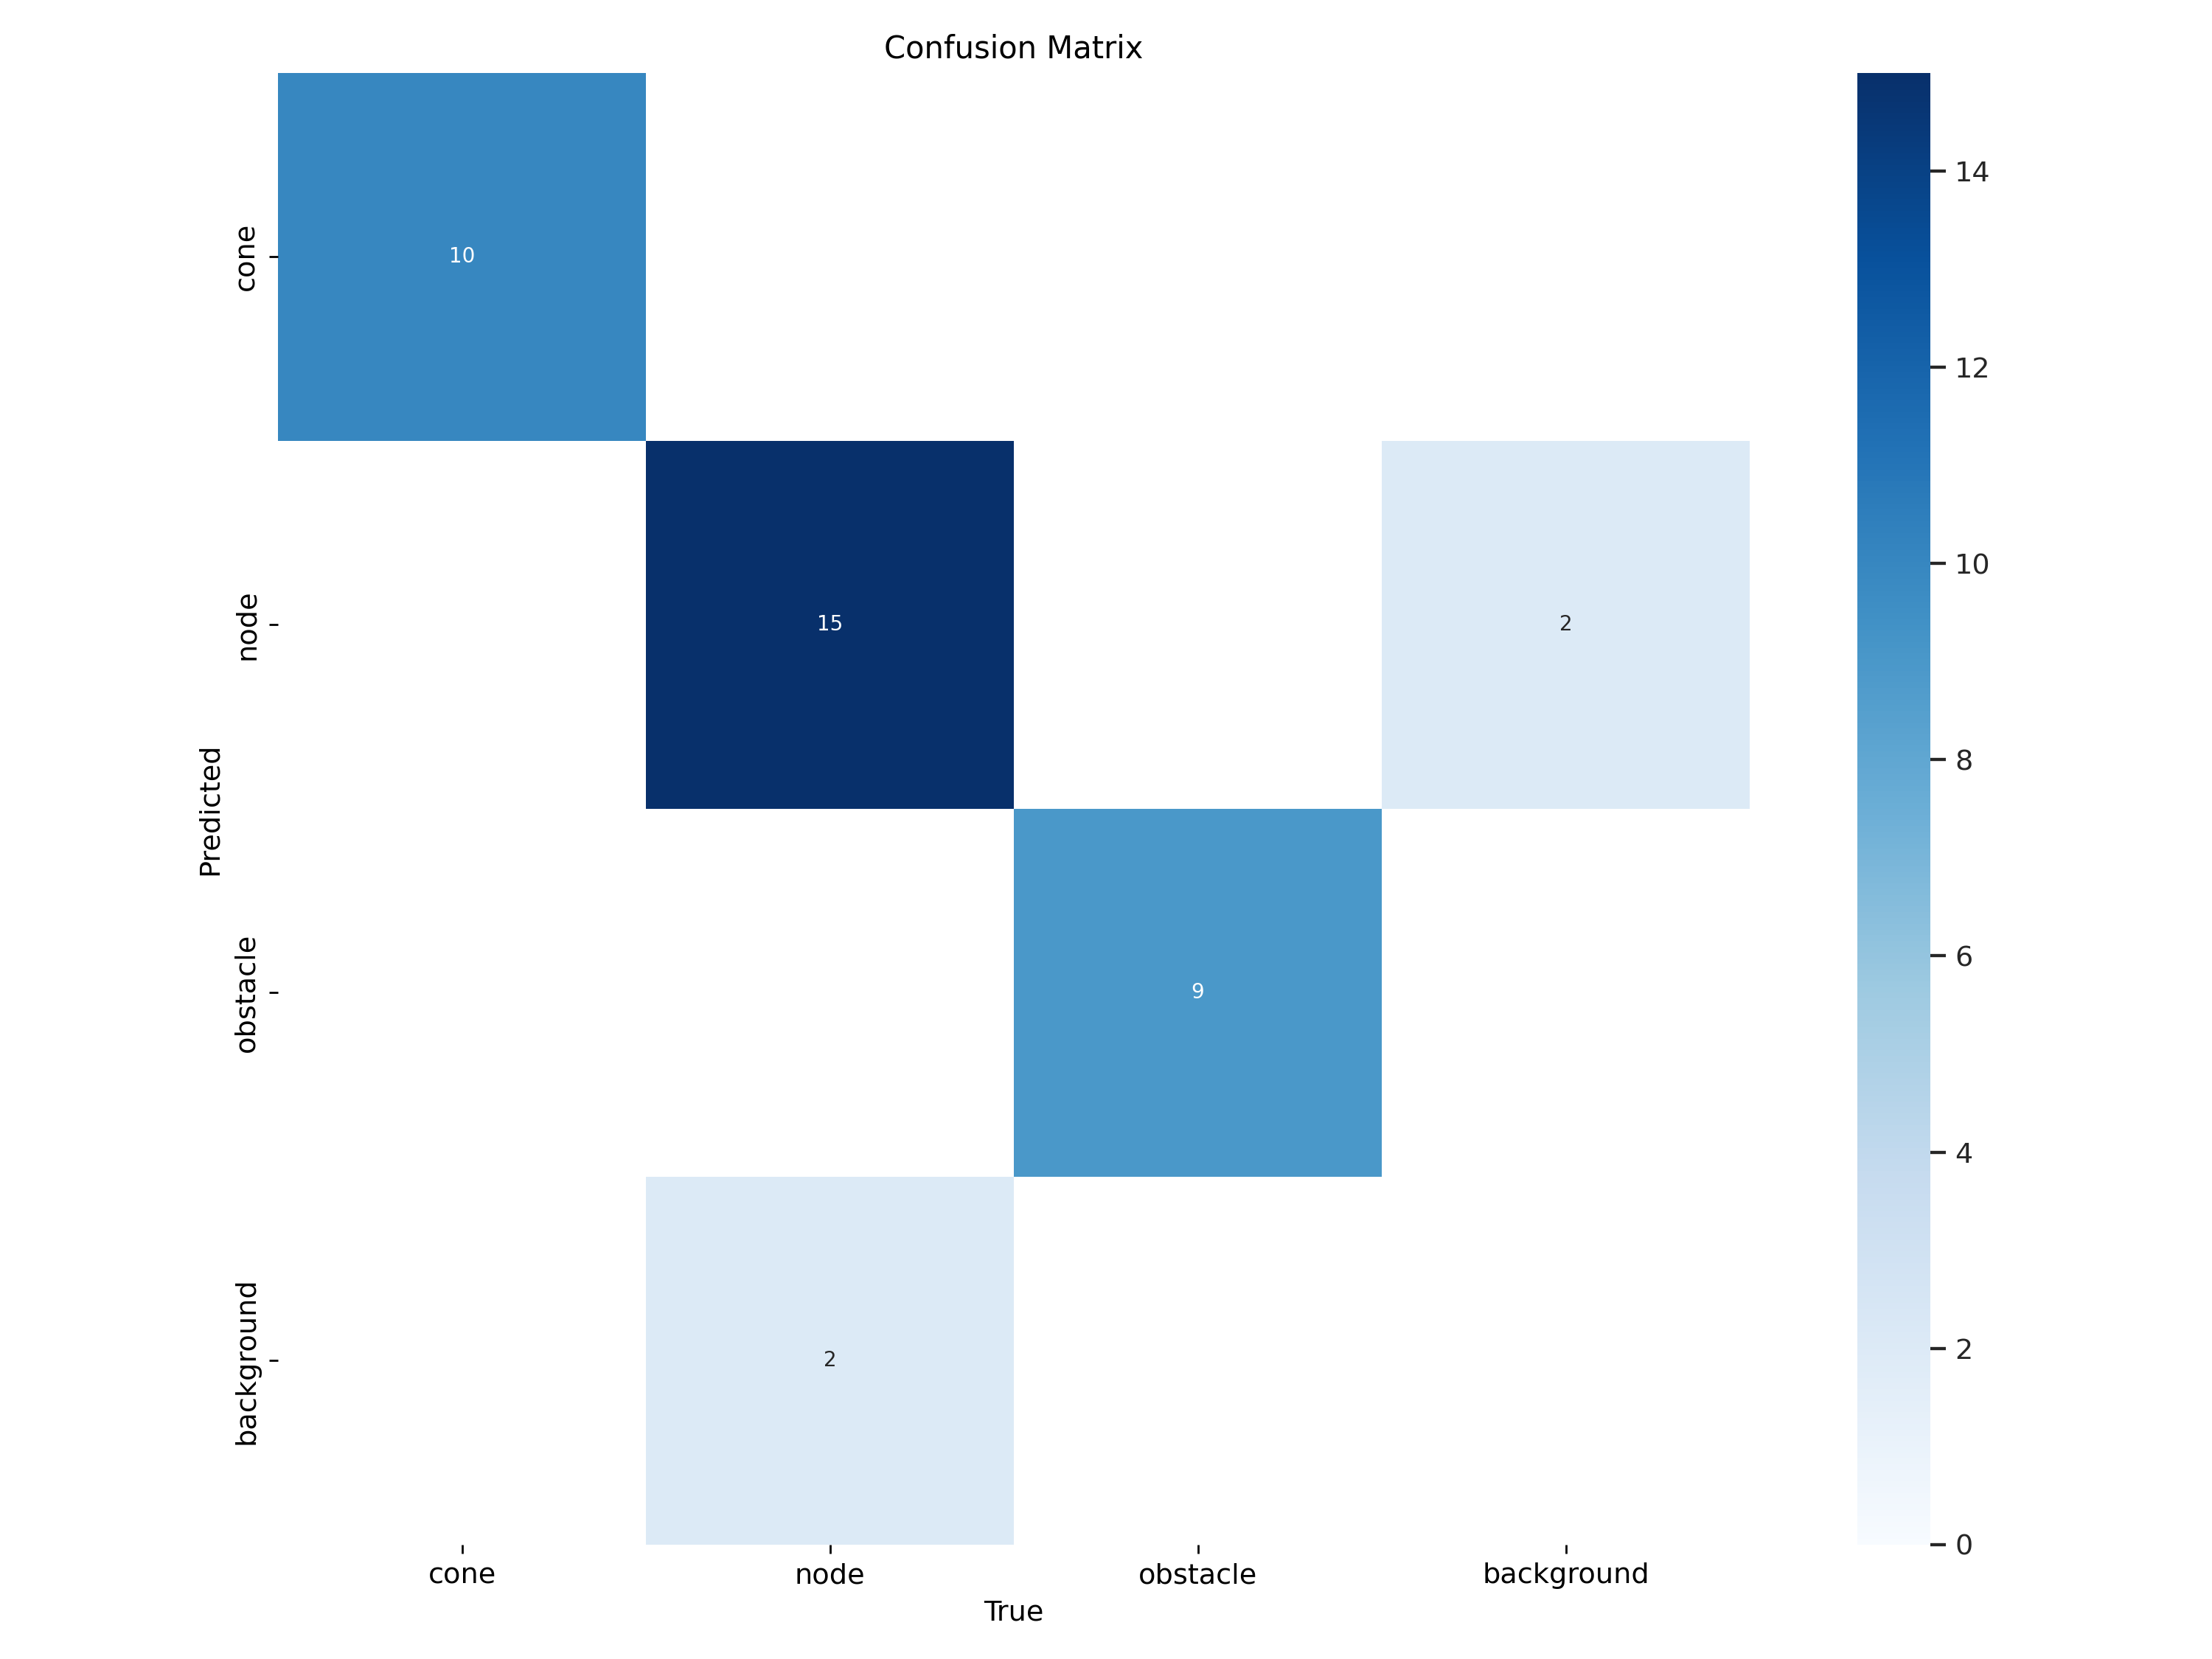
\includegraphics[width=10cm]{assets/IT/yolo/confusion_matrix.png}
\caption{Confusion Matrix Bilderkennung}
\label{fig:conf-matrix-model}
\end{figure}

Es kann ein Ziel ausgewählt werden und der Roboter kann gestartet werden. Die Zielknoten können zuverlässig erkannt werden, was mit realistischen Tests geprüft wurde. Der Buzzersound, der angibt, dass das Ziel erreicht wurde, ertönt schnell und laut.

Der Roboter kann über einen Schalter ein- und ausgeschaltet werden.

Die Konstruktionswerkstoffe konnten wie in PREN1 vorgesehen unter Berücksichtigung der im Kapitel \ref{nachhaltigkeit} Nachhaltigkeit aufgeführten Kriterien ausgewählt werden.

Obwohl fast alle einzelnen Anforderungen erfüllt werden konnten, kann der Roboter momentan nicht das Wegenetz durchqueren. Die Steuerung konnte bis jetzt noch nicht zusammengefügt werden. Die Navigation und die Mechanik funktionieren jedoch beide als Teilsystem.
    \section{Nachhaltigkeit}
(noch nicht fertig Timo)

Trotz der Herausforderungen in der Umsetzung konnte ein grosser Teil der in PREN1  definierten Nachhaltigkeitsziele (referenzieren) erfüllt werden. Das Projekt hat gezeigt, dass auch in technisch anspruchsvollen Studierendenprojekten nachhaltiges Handeln möglich und praktikabel ist.

\subsection{3R-Prinzip: Reduce, Reuse, Recycle}
Die in PREN1 definierten Nachhaltigkeitsprinzipien,insbesondere die 3 R (Reduce, Reuse, Recycle), wurden auch in der praktischen Umsetzung in PREN2 angewendet.  

 In diesem Kapitel wird erläutert wie die drei Rs im Verlauf des Semesters umgesetzt wurden.

\subsubsection{Reduce}

% Wie im pren1

Zur weiteren Reduktion des Ressourcenverbrauchs wurde auf papierlose Zusammenarbeit gesetzt. Die gesamte Kommunikation und Dokumentation erfolgte digital. Eine eigene Overleaf-Instanz für die LaTeX-Dokumentation wurde auf einem bereits laufenden Server betrieben, wodurch zusätzlicher Stromverbrauch vermieden werden konnte. Auch das tägliche PDF-Building der Dokumentation wurde bewusst auf ein Minimum reduziert.

Viele Bauteile wie Sensoren, Steckbrettmaterialien, PLA-Filament oder Endschalter waren bereits im Besitz einzelner Teammitglieder und konnten direkt verwendet werden. Dadurch konnten nicht nur unnötige Bestellungen, sondern auch Verpackungsmaterial, Transportwege und Kosten reduziert werden.


\subsubsection{Reuse}

Im Bereich Reuse wurden zahlreiche Elemente des Prototypings direkt in den finalen Roboter übernommen. Dazu zählen etwa die Räder, der Kameraturm und der Greifer. Auch Elektronikkomponenten wie der Raspberry Pi, Sensoren und die Kamera wurden teilweise aus bereits vorhandenen Beständen eingebracht. Die modulare Bauweise erlaubte es, einzelne Bauteile mehrfach zu verwenden und flexibel anzupassen. Beispielsweise konnte die Grundplatte mehrfach verändert werden, ohne ersetzt werden zu müssen. Auch das Konzept, mehrere kleine statt einer grossen Leiterplatte zu verwenden, wurde aus Nachhaltigkeitsgründen beibehalten.



Die Grundplatte des Prototyps aus PREN1 wurde so konstruiert, dass sie modular erweiterbar ist. Zusätzliche Bohrungen und Nuten konnten während der Entwicklung fortlaufend eingebracht werden, ohne dass eine neue Platte gefertigt werden musste. Die Nachbearbeitung mittels Laserschneidmaschine verlief dabei ohne technische Probleme. Dadurch konnte der Materialeinsatz auf eine einzige Grundplatte beschränkt und die Entstehung von Abfall minimiert werden. Eine Übersicht der verschiedenen Bearbeitungszustände ist in Abbildung \ref{fig: Weiterentwicklung der Grundplatte} dargestellt.

\begin{figure}[H] % oder [htbp]
    \centering
    \begin{subfigure}[b]{0.45\textwidth}
        \centering
        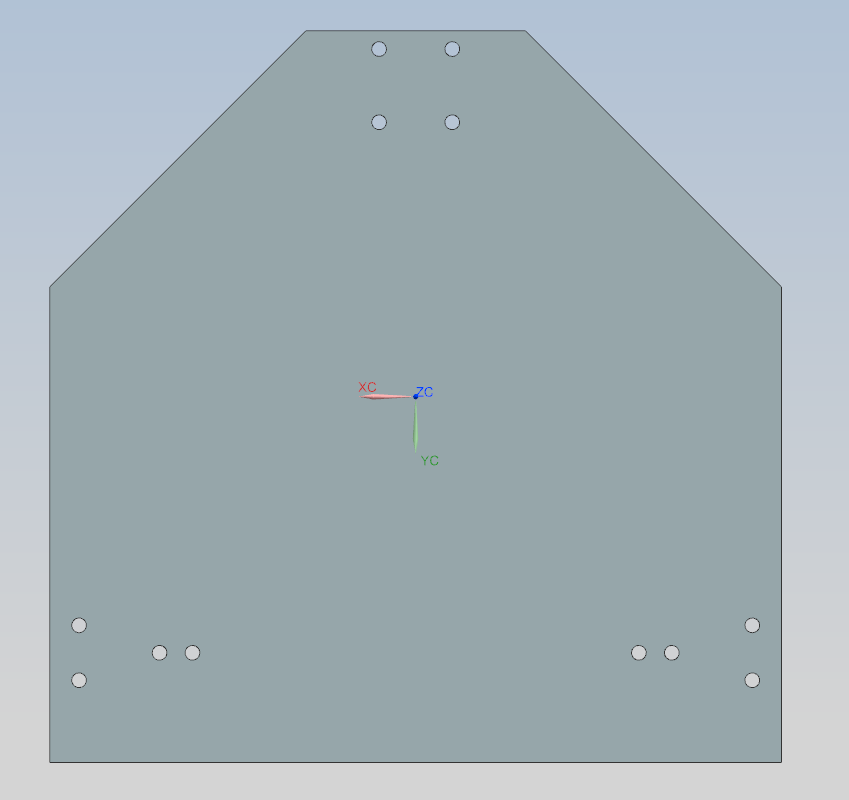
\includegraphics[width=\linewidth]{assets/MT/Grundplatte_V0.png}
        \caption{Grundplatte V0}
    \end{subfigure}
    \hfill
    \begin{subfigure}[b]{0.45\textwidth}
        \centering
        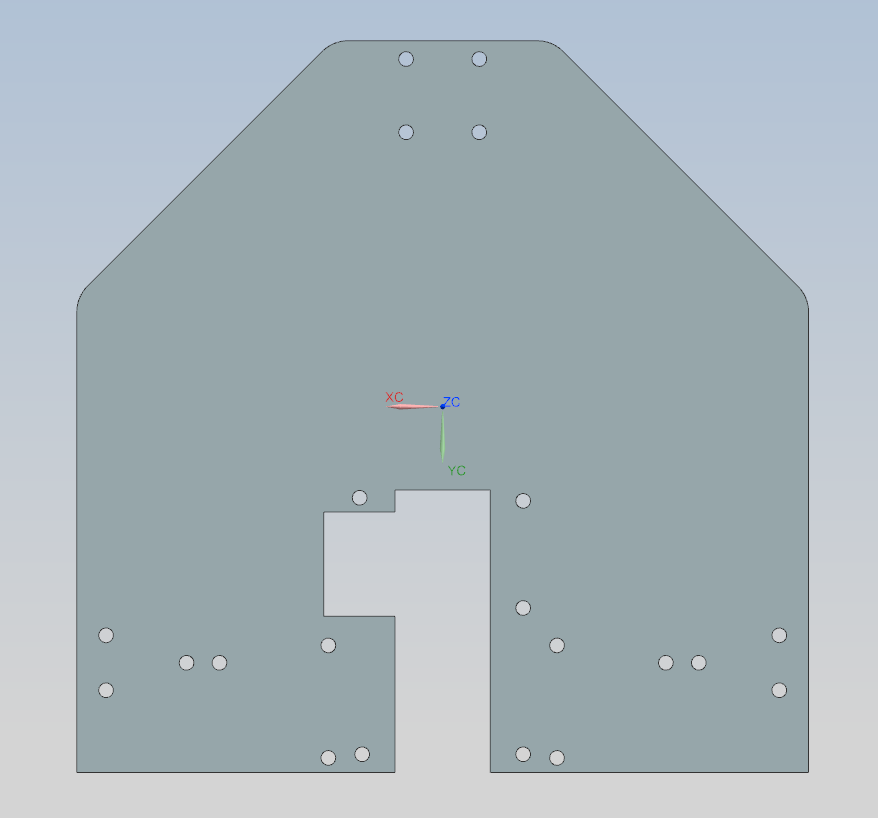
\includegraphics[width=\linewidth]{assets/MT/Grundplatte_V1.png}
        \caption{Grundplatte V1}
    \end{subfigure}

    \vspace{0.5cm}

    \begin{subfigure}[b]{0.45\textwidth}
        \centering
        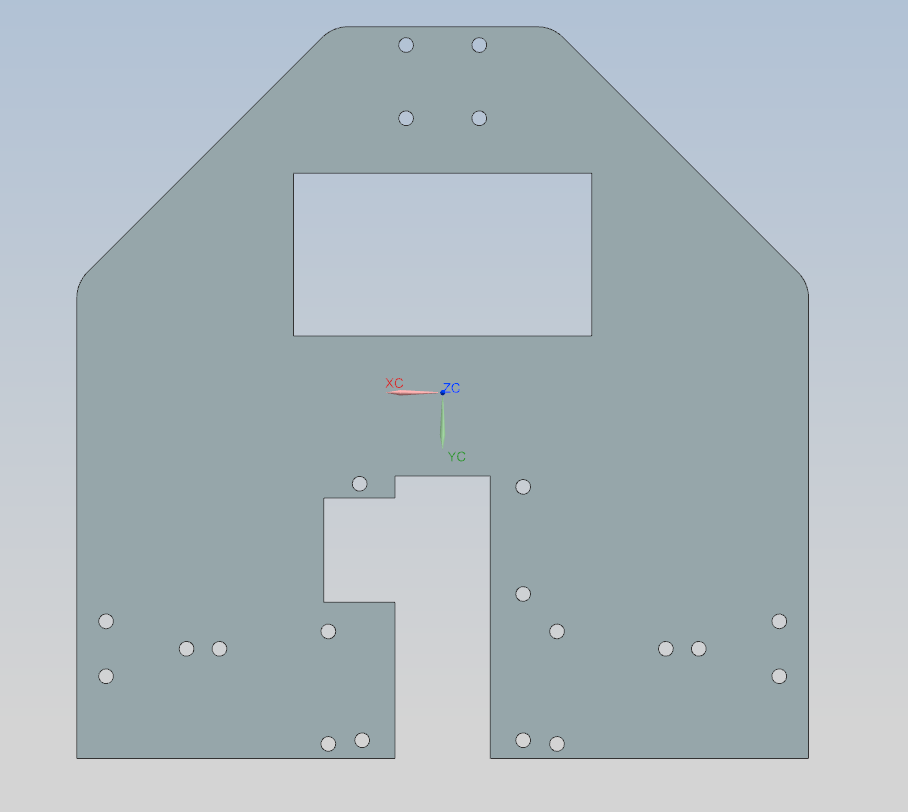
\includegraphics[width=\linewidth]{assets/MT/Grundplatte_V2.png}
        \caption{Grundplatte V2}
    \end{subfigure}
    \hfill
    \begin{subfigure}[b]{0.45\textwidth}
        \centering
        \includegraphics[width=\linewidth]{assets/MT/Grundplatte_V3.png}
        \caption{Grundplatte V3}
    \end{subfigure}
    \caption{Weiterentwicklung der Grundplatte}
    \label{fig: Weiterentwicklung der Grundplatte}
\end{figure}


\subsubsection{Recycle}

Durch die modulare Bauweise ist der Roboter nach Gebrauch auch wieder komplett zerleg
bar. Materialien und Komponenten, welche nicht wiederverwendet werden können, können einzeln recycelt werden.

\subsection{Ökobilanz und Materialanalyse}

\subsubsection{Betrachtung hinsichtlich Ökobilanz}
% Beschreibung des Gesamtgewichtes und der drei größten Material-Positionen
Das Gesamtgewicht des Fahrzeugs beträgt \textbf{1.262 Kg}. In folgender Tabelle werden die drei grössten Material-Positionen in Kilogramm und Prozent des Gesamtgewichtes aufgelistet, gefolgt von einer Beschreibung der Recyclingfähigkeit, Entsorgung und/oder Abfallbehandlung dieser Materialien.

\begin{table}[h]
\centering
\caption{Material-Positionen nach Gewichtsanteil}
\begin{tabular}{l c c p{5cm}}
\toprule
Material & Gewicht  & Anteil (\%) & Beschreibung der Recyclingfähigkeit/Entsorgung \\
\midrule
\acrshort{mdf} & 0.166 Kg & 13\% & Recycelbar aber schwierig \\
\acrshort{pla} & 0.252 Kg & 20\% & Gut Recycelbar \\
Batterie & 0.202 Kg & 16\% & Recyceln möglich aber ist teuer \\
\bottomrule
\end{tabular}
\end{table}

\subsubsection{Nachhaltig-kritischste Materialien}
% Auflistung und Beschreibung der nachhaltig-kritischsten Materialien
Im Folgenden werden mindestens drei der nachhaltig-kritischsten Materialien, die im Fahrzeug verbaut sind, aufgelistet. Für jedes Material wird erläutert, warum es nicht nachhaltig ist, und es werden mögliche Massnahmen zur Vermeidung vorgeschlagen.

\begin{itemize}
    \item \textbf{Material 1:} \acrfull{mdf} \\
          \textit{Grund der mangelnden Nachhaltigkeit:} Hoher Energieaufwand und vergleichbar hoher Leimanteil  \\
          \textit{Vermeidungsstrategie:} Leimholzplatten mit weniger Leimanteil oder Massivholzplatten verwenden. Ökolgisch zertifiziertes MDF ist nachhaltiger
          
    \item \textbf{Material 2:} Lithium in der Batterie \\
          \textit{Grund der mangelnden Nachhaltigkeit:} Lithium ist umweltschädlich bei der Herstellung. Abbau und Raffinerie benötigt viel Energie und Wasser und setzt Schadstoffe frei. \\
          \textit{Vermeidungsstrategie:} Lithium für Batterien ist praktisch nicht vermeidbar wenn eine Batterie benötigt wird. Der Herstellungsprozess kann jedoch umweltfreundlicher gestaltet werden
          
    \item \textbf{Material 3:} Kupfer in Kabel \\
          \textit{Grund der mangelnden Nachhaltigkeit:} Kupfer ist umweltschädlich bei der Herstellung. Abbau und Raffinerie benötigt viel Energie und Wasser und setzt Schadstoffe frei. \\
          \textit{Vermeidungsstrategie:} Kabel und Leitungen von Hersteller beziehen welche ausschliesslich recycletes Kupfer verwenden.
\end{itemize}


    \section{Schlussdiskussion}

In den folgenden Kapiteln wird zusammengefasst, was in \acrshort{pren2} bearbeitet wurde mit Ausblick auf den Wettbewerb.
Ebenfalls werden die gesammelten Erfahrungen bezüglich der Arbeiten und der Zusammenarbeit im Team beschrieben und welche Lehren daraus gezogen werden konnten.

\subsection{Erfüllung der Anforderungen}

Der Roboter kann die einzelnen benötigten Funktionen umsetzen:

\begin{itemize}
    \item Der Roboter kann eine bestimmte Distanz vorwärts und rückwärts fahren.
    \item Der Roboter kann sich drehen.
    \item Der Roboter kann einer Linie folgen.
    \item Der Roboter kann anhalten, sobald er sich auf einem Knoten befindet.
    \item Der Roboter greift das Hindernis, sobald er es am Endschalter spürt.
    \item Der Roboter kann, sobald er ein Hindernis am Endschalter spürt, einen Prozess starten, um das Hindernis zu beseitigen. Das Hindernis wird am selben Ort wieder abgestellt.
    \item Der Roboter kann mit einem Ultraschall Objekte vor sich bemerken.
    \item Der Roboter kann ein Bild machen von einem Knoten und die Winkel der ausgehenden Linien erkennen.
    \item Der Roboter kann ein Bild machen zu einem Nachbarsknoten und erkennen, ob sich eine Pylone, eine Barriere oder nur ein Knoten dort befindet.
    \item Der Roboter kann den schnellsten Weg zum Ziel finden.
    \item Es kann ein Ziel ausgewählt werden.
    \item Der Roboter kann mit einem Notstop ausgeschaltet werden.
    \item Der Roboter kann erkennen, wenn er sich im Ziel befindet.
    \item Der Roboter kann mit einem Buzzergeräusch zeigen, dass er sich im Ziel befindet.
\end{itemize}

Die einzelnen Funktionen der Steuerung konnten jedoch noch nicht zusammengesetzt werden.

Die Navigation wurde trotzdem getestet ohne ein Fahrwerk, der Kameraturm wurde an die Orte geschoben, welche die Navigation vorgibt. Mit den Instruktionen der Navigation konnte der Graph erfolgreich traversiert werden. Dieser Test ist im Anhang beschrieben in Kapitel \nameref{statische-traver}. Auch die Mechanik konnte erfolgreich umgesetzt werden. Der Roboter fährt und dreht sich stabil, der Greifmechanismus funktioniert und alle Komponenten unterstützen die Funktionen erfolgreich.

Die nicht-funktionalen Anforderungen konnten ebenfalls erreicht werden: Die maximale Grösse wurde eingehalten und das Gewicht wurde klar unterschritten. Der Roboter ist robust gebaut und durch die Verwendung von \acrshort{pla} konnte nachhaltiger gearbeitet werden. Auch das Budget konnte eingehalten werden.

\subsubsection{Ausblick}

Die Funktionen konnten implementiert werden, jedoch muss zwingend noch daran gearbeitet werden, sodass es als Komplettsystem funktioniert. Die nächsten Wochen werden dafür verwendet, dies noch zu implementieren.

\textbf{Risiken}

Die folgenden Risiken aus der Risikobewertung bestehen noch für den Wettbewerb. 

\begin{itemize}
    \item Risiko 2: Knoten werden nicht erkannt
    \item Risiko 8: Hindernisse werden beim Anheben verschoben.
    \item Risiko 12: Roboter wählt falschen Pfad.
\end{itemize}

Jedoch ist das relevanteste Risiko, das es in den folgenden Wochen gilt zu beseitigen, dass die Zeit nicht mehr reichte, die einzelnen Steuerungsfunktionen zusammenzusetzen.
Bei dem Zusammensetzen werden wahrscheinlich weitere Probleme auftreten, die innert kurzer Zeit behoben werden müssen.



\subsection{Lessons Learned}

Die während PREN2 aufgetretenen Hindernisse, führten zu wichtigen Learnings, die in künftigen Projekten früher erkannt oder umgangen werden können.

Das Konzept aus \acrshort{pren1} dient als Basis für den Roboterbau. Es gab Momente, in denen festgestellt wurde, dass Teile des Konzeptes nicht so funktionieren, wie geplant. Dies passierte beispielsweise bei der Messung der Distanz zu dem nächsten Knoten. Die funktioniert technisch zwar, war aber zu riskant, da der Knoten selber nicht immer genau erkannt wurde. Deshalb wurde das Konzept hier angepasst. Die Herausforderung dabei ist es, dass das neue Konzept in das Gesamtkonzept passen muss. Wir haben gelernt mit unerwarteten Problemen auf angemessene Art umzugehen.

Ein weiteres Hindernis war das parallele Arbeiten. Zu Beginn hatten wir mehrere Prototypen des Roboters, die einzelne Teilfunktionen ausführen konnten. Ab einem gewissen Stand der Systemintegration konnte der Roboter nur noch als ganzes getestet werden. Es musste koordiniert werden, wer wann welche Tests durchführt. Der Test der Navigation wurde schlussendlich mit der Hilfe von der Kamerahalterung aus PREN1 durchgeführt, so konnten parallel mehrere Tests durchgeführt werden.

Im Verlauf des Projekts wurde deutlich, wie wichtig die Technologierecherche in \acrshort{pren1} war. Rückblickend hätte eine intensivere Recherche in bestimmten Bereichen in \acrshort{pren2} von grossem Nutzen sein können. Insbesondere beim Problem mit den Encoder Motoren. Für zukünftige Projekte sollte allgemein beim auftretenden von Problemen frühzeitig parallel an der Fehleranalyse gearbeitet und gleichzeitig eine alternative Lösung erarbeitet werden. Dieses Vorgehen hätte geholfen die Implementierung des Gyroskop früher in Betracht zu ziehen.




    % 

\section{Template}
\subsection{Some subsection}
Lorem ipsum dolor sit amet, officia excepteur ex fugiat reprehenderit enim labore culpa sint ad nisi Lorem pariatur mollit ex esse exercitation amet. Nisi anim cupidatat excepteur officia. Reprehenderit nostrud nostrud ipsum Lorem est aliquip amet voluptate voluptate dolor minim nulla est proident. Nostrud officia pariatur ut officia. Sit irure elit esse ea nulla sunt ex occaecat reprehenderit commodo officia dolor Lorem duis laboris cupidatat officia voluptate. Culpa proident adipisicing id nulla nisi laboris ex in Lorem sunt duis officia eiusmod. Aliqua reprehenderit commodo ex non excepteur duis sunt velit enim. Voluptate laboris sint cupidatat ullamco ut ea consectetur et est culpa et culpa duis.

\subsection{Another subsection: Liste}
How to make a bullet-point list.
\begin{itemize}
    \item First item
    \item Second item
    \item Third item
\end{itemize}

 And another one:
 
\begin{itemize}
    \item First item
    \item Second item
\end{itemize}
\subsection{Third subsection: Nummerierte Liste}
How to make a numbered list:
\begin{enumerate}
    \item First enum
    \item Second enum
    \item Third enum
\end{enumerate}
\subsubsection{Some sub-subsection}
Lorem ipsum dolor sit amet, qui minim labore adipisicing minim sint cillum sint consectetur cupidatat.


\subsection{Some subsection: Bild einfuegen}
Lorem ipsum dolor sit amet, officia excepteur ex fugiat reprehenderit enim labore culpa sint ad nisi Lorem pariatur mollit ex esse exercitation amet. Nisi anim cupidatat excepteur officia. Reprehenderit nostrud nostrud ipsum Lorem est aliquip amet voluptate voluptate dolor minim nulla est proident. Nostrud officia pariatur ut officia. Sit irure elit esse ea nulla sunt ex occaecat reprehenderit commodo officia dolor Lorem duis laboris cupidatat officia voluptate. Culpa proident adipisicing id nulla nisi laboris ex in Lorem sunt duis officia eiusmod. Aliqua reprehenderit commodo ex non excepteur duis sunt velit enim. Voluptate laboris sint cupidatat ullamco ut ea consectetur et est culpa et culpa duis.

\begin{figure}[h]
\centering
\includegraphics[width=\textwidth]{img/HSLU_Logo.png}
\caption{Sample caption}
\label{fig:hslu-logo}
\end{figure}

Here we can reference image \ref{fig:hslu-logo} if a label has been defined when inserting the image. If you do this it will be uniform.

\subsubsection{Some sub-subsection: Tabelle}

This is how you make a table and reference it like this: \ref{table:template}:

\begin{table}[h!]
\centering
\begin{tabular}{ |l| l| l|} % Dimension breite
  \textbf{Column Header 1} & \textbf{Column Header 2} &  \textbf{Column Header 3}\\
  \hline
  
  Row 1, Col1 & Row 1, Col 2 & Row 1, Col 3\\

  Row 2 &Row 2 & Row 2 \\
  
  Row 3 & Row 3 & Row 3 \\
  
  
  Only fill first Col && and the last\\
\end{tabular}
\caption{Table to show how to use tables}
\label{table:template}
\end{table}

\subsection{Subsection: Akronyme und Quellen}

For acronym entries, add them to the ``glossary.tex'' file and reference them like this: \acrfull{pren1} when you use them for the first time.

When you wanna use the short form do this \acrshort{pren1}.

How to use a source\cite{wikipedia-scrum}.

\subsection{Subsection: Quotes/Anführungszeichen}

\verb|"Plug and Play" --> Falsche Quotes -->| "Plug and Play"

\verb|‘Plug and Play’ --> doppelte Quotes -->| ‘Plug and Play’

\verb|‘‘Plug and Play’’ --> Einfache Quotes -->| “Plug and Play”

oder für Deutsche Grammatik:

\verb|\enquote{Plug and Play} -->| \enquote{„Plug and Play“}


%%%%%%%%%%%%%%%%%%%%%%%%%%%%%%%%%%%%%%%%%%%%%%%%%%%%%%%%%%%%%%%%%%%%%%%%%%%%%%%%%%%%%%%%%%
%%%%%%%%%%%%%%%%%%%%%%%%%%%%%%%%%%%%%%%%%%%%%%%%%%%%%%%%%%%%%%%%%%%%%%%%%%%%%%%%%%%%%%%%%%
%%%%%%%%%%%%%%%%%%%%%%%%%%%%%%%%%%%%%%%%%%%%%%%%%%%%%%%%%%%%%%%%%%%%%%%%%%%%%%%%%%%%%%%%%%


    % TODO Glossary is ugly
    \newpage
    \addglossary
    \printglossary[]


    % Literaturverzeichnis
  \setcounter{biburllcpenalty}{7000}
  \setcounter{biburlucpenalty}{8000}
  \newpage
  \addcontentsline{toc}
    {section}
    {Literatur}
  \printbibliography[
    heading=subbibliography
  ]

  % Anhang

  \newpage

\section*{Anhang}
  \addcontentsline{toc}
    {section}
    {Anhang}



\subsection*{Elektronischer Anhang}\label{elect-anhang}
\addcontentsline{toc}
{subsection}
{Elektronischer Anhang}

Diese Dokumentation wurde zusammen mit einem elektronischen Anhang in Form einer ZIP-Datei abgegeben. Darin befinden sich der Simulator Programmiercode inklusive dessen Ergebnisse und die erstellten CAD Dateien.

TODO LIST OF WHATS IN THERE

\newpage
\subfile{parts/x-projektplanung}
\newpage

%%%%%%%%%%%%%%%%%% Aufgabenstellung

\subsection*{Originale Aufgabenstellung}\label{aufgabenstellung}
\addcontentsline{toc}
{subsection}
{Originale Aufgabenstellung}

Nachfolgend ist die originale Aufgabenstellung angehängt.

\includepdf[pages=-]{assets/projektmanagement/AufgabenstellungPREN1HS24.pdf}

%%%%%%%%%%%%%%% Anforderungsliste %%%%%%%%%%%%%%%%%%%%%%%%%

\subsection*{Anforderungsliste}\label{anforderungliste}
  \addcontentsline{toc}
    {subsection}
    {Anforderungsliste}
Die  Anforderungsliste ist ersichtlich in Tabellen \ref{table:anforderungsliste_page1} und \ref{table:anforderungsliste_page2}.

\begin{table}[H]
\centering
\includegraphics[width=\textwidth]{assets/projektmanagement/Anforderungsliste_V1.01_page1.pdf}
\caption{Anforderungsliste Teil 1}
\label{table:anforderungsliste_page1}
\end{table}
\newpage

\begin{table}[H]
\centering
\includegraphics[width=\textwidth]{assets/projektmanagement/Anforderungsliste_V1.01_page2.pdf}
\caption{Anforderungsliste Teil 2}
\label{table:anforderungsliste_page2}
\end{table}
\newpage


%%%%%%%%%%%%%%%% Model Evaluation %%%%%%%%%%%%%%%%%%%%%%%%%5

\subsection*{YOLOv11 Model Evaluation}\label{model-evaluation}
  \addcontentsline{toc}
    {subsection}
    {YOLOv11 Model Evaluation}

Damit Pylonen, Barrieren und Knoten erkannt werden können, wird ein Model trainiert. Insgesamt wurden über 30 verschiedene YOLO Models trainiert. Viele davon wurden bereits in einem vorherigen Schritt aussortiert, da einige sehr offensichtlich schlechte Performance aufwiesen aufgrund davon, wie es die Objekte erkannt, beziehungsweise nicht erkannt hat. Auf der folgenden Seite ist eine Tabelle angehängt, in der die relevanten Models miteinander verglichen werden und das beste Model gewählt wurde.

Die Model Performance wird an folgenden Parametern gemessen:\cite{model-performance}

\begin{itemize}
    \item Confusion Matrix: Zeigt was das Model vorhergesagt hat und was tatsächlich zu sehen war. Je 'diagonaler' die Matrix, desto besser.
    \item F1-Confidence: Zeigt die Balance zwischen Confidence (Wahrscheinlichkeit, dass Vorrausgesagtes stimmt) und F1 Score (Harmonischer Durchschnitt von Recall und Precision). Je höher der F1 Wert, desto besser.
    \item Precision-Confidence: Zeigt die Balance zwischen Precision (Anteil von 'True Positives'; wenn Model sagt, es gibt einen Knoten, wie akkurat ist diese Deutung?) und Confidence. Je tiefer die Confidence, desto besser, da dadurch der hoechste Praezisionswert bereits bei einer tieferen Confidence erreicht wird.
    \item Precision-Recall: Zeigt die Balance zwischen Precision und Recall (Faehigkeit, alle Instanzen zu erkennen). Je hoeher die Precision, desto besser.
    \item Recall-Confidence: Zeigt die Balance zwischen Recall und Confidence. Je höher der Recall, desto besser.
    \item Lernverlauf: Zeigt inwiefern der Verlust (Unterschied zwischen Vorhergesagtem und Realität) sinkt bei den Trainingsdaten und den Validationsdaten. Beginnt der Verlust bei der Validation zu steigen, deutet dies auf Overfitting hin\footnote{https://developers.google.com/machine-learning/crash-course/overfitting/overfitting}. Sollte exponentiell sinken. Zeigt, wie das Model und Wissen gewinnt. Sollte exponentiell steigen.
\end{itemize}


Der Vergleich zwischen mehreren potentiellen Modellen ist in folgendem Dokument ersichtlich. Zwei Modelle wurden jeweils verglichen aufgrund von mehreren Werten. Ist der jeweilige Wert des einen Models besser, wird diese Zelle grün eingefärbt.

Es wurde untersucht, ob das Modell bessere Ergebnisse bringt, wenn die beiden Barrieren pro Farbe in einzelnen Klassen aufgeteilt werden oder nicht und verschiedene Augmentationen wurden verglichen. Augmentationen werden auf die Trainingsbilder angewandt, damit diese diverser sind und zum einen mehr der Realitaet entsprechen und auch um mehr Trainingsmaterial zu haben. Ebenfalls wurde experimentiert mit unterschiedlichen Grössen der Bilder. 

\includepdf[pages=-]{assets/IT/testing/yolo/ModelComparison.pdf}


%%%%%%%%%%%%%%%%%%%%%%%%%%%target node%%%%%%%%%%%%%%%%%%%%%%%%%%%%%

\subsection*{Zielknotenerkennung}\label{target-node-unittests}
  \addcontentsline{toc}
    {subsection}
    {Zielknotenerkennung}

Die Tests der Zielknotenerkennung haben zwei Ziele:

\begin{enumerate}
    \item Parameter tunen.
    \item Funktionalitaet testen.
\end{enumerate}

\textbf{Parameter tunen}

Die Zielknotenerkennung hat folgende Parameter, deren Werte durch Tests optimiert wurden. Ein Match bezeichnet einen gefundenen Erkennungspunkt des Buchstabens. Auf dem folgenden Bild \ref{img:orb-example} gibt es beispielsweise 14 Matches (Linien), deren Durchschnittliche Distanz 0 ist, da es sich um das selbe Bild handelt. Die Erkennungspunkte sind im Bild links gleich weit voneinander entfernt wie im rechten.

\begin{figure}[H]
\centering
\includegraphics[width=5cm]{assets/IT/testing/target_node/orb-a.png}
\caption{Beispielbild mit Erkennungspunkten 'Matches'}
\label{img:orb-example}
\end{figure}

\begin{enumerate}
    \item MIN\_MATCHES\_REQUIRED = 10: Wie viele Matches muss es geben?
    \item MAX\_DISTANCE\_ALLOWED = 50: Wie ungenau dürfen die Matches maximal sein?
    \item Differenz Messpunkte < 5: Differenz der Anzahl Matches für jeden Buchstaben, um die Buchstaben mit den zwei meisten Matches vergleichen zu müssen, anstatt direkt den Buchstaben mit den meisten Matches zu nehmen.
    \item Distanz der Distanz > 5: Differenz in der durchschnittlichen Distanz der Matches der zwei Buchstaben mit den meisten Matches. Hat der Buchstaben mit weniger Matches eine Distanz, die mindestens 6 kleiner ist, passt dieser besser.
\end{enumerate}

Die finalen Werte wurden mithilfe von diesen Testresultaten in Tabelle \ref{letter-matches-orb} ermittelt. Ist die Anzahl Match Differenz grösser als 5, wird die Distanz von zwei Buchstaben gemessen.  Ist die Differenz der Distanzen grösser als 5, wird der zweite Buchstabe genommen. Werden benötigte Anzahl Matches nicht erreicht oder wird die maximale Distanz überschritten, wird kein Buchstabe erkannt.

\begin{table}[H]
\centering
\small
\begin{tabularx}{\textwidth}{|c|X|X|c|X|c|}
\hline
\textbf{Buchstabe} & \textbf{Anzahl Matches pro Buchstabe} & \textbf{Anzahl Match Differenz} & \textbf{Distanz} & \textbf{Differenz Distanz} \\
\hline
None & {'A': 5, 'B': 5, 'C': 5} & 0 &  &  \\
\hline
A & {'A': 135, 'B': 42, 'C': 22} & 93 & A: 0.00 &  \\
\hline
B & {'B': 221, 'C': 51, 'A': 42} & 170 & B: 0.00 &  \\
\hline
C & {'C': 173, 'B': 51, 'A': 22} & 122 & C: 0.00 &  \\
\hline
None & {'B': 11, 'A': 10, 'C': 10} & 1 & B: 72.45, A: 63.30 & \textit{Distanzen > 50}\\
\hline
A & {'A': 21, 'B': 11, 'C': 9} & 10 & A: 18.80 &  \\
\hline
B & {'B': 25, 'A': 12, 'C': 10} & 13 & B: 13.80 &  \\
\hline
B & {'B': 28, 'A': 21, 'C': 15} & 7 & B: 15.70 &  \\
\hline
C & {'A': 24, 'C': 23, 'B': 18} & 1 & A: 45.58, C: 32.61 & 12.97 \\
\hline
C & {'B': 22, 'C': 22, 'A': 13} & 0 & B: 35.41, C: 29.77 & 5.64 \\
\hline
C & {'B': 19, 'C': 15, 'A': 13} & 4 & B: 23.30, c: 29.01 & 5.71 \\
\hline
A & {'A': 26, 'C': 14, 'B': 12} & 12 & A: 22.30 &  \\
\hline
A & {'A': 20, 'B': 13, 'C': 9} & 7 & A: 16.30 &  \\
\hline
A & {'A': 24, 'B': 12, 'C': 10} & 12 & A: 16.10 &  \\
\hline
B & {'B': 28, 'A': 22, 'C': 15} & 6 & B: 15.80 &  \\
\hline
\end{tabularx}
\caption{Analyse der Buchstaben-Matches mit Distanzen}
\label{letter-matches-orb}
\end{table}

\textbf{Funktionalität testen}

Die Logik, um den richtigen Buchstaben zu erkennen beschränkt sich nicht nur auf den \acrshort{orb} Algorithmus. Es wurde selber noch ein Algorithmus implementiert. Grundsätzlich wird der Buchstabe, für den die meisten Matches gefunden wurden, zurückgeben. Jedoch ist es vor allem bei dem Buchstaben C so, dass es relativ wenige Messpunkte gibt, da der Buchstaben sehr simpel ist. Das heisst, wenn C erkannt werden soll, gibt es oft falsche Buchstaben, mit mehr Messpunkten. Falls die Buchstaben mit den meisten und den zweit meisten Messpunkten nur 5 Messpunkte auseinander liegen, werden die Distanzen der Messpunkte verglichen. Wenn der Buchstaben, der maximal 5 Messpunkte weniger hat, eine durchschnittliche Distanz von mehr als 5 hat, wird der Buchstaben zurückgegeben, mit den wenigeren Messpunkten. Diese Logik wird in den Unittests getestet.

Die folgenden Fälle wurden getestet:

\begin{enumerate}
    \item Buchstabe A ist ersichtlich (verschiedene Rotationen): Optimale Verhältnisse \& realistische Verhältnisse.
    \item Buchstabe B ist ersichtlich (verschiedene Rotationen): Optimale Verhältnisse \& realistische Verhältnisse.
    \item Buchstabe C ist ersichtlich (verschiedene Rotationen): Optimale Verhältnisse \& realistische Verhältnisse.
    \item Kein Buchstabe ist ersichtlich: Optimale Verhältnisse \& realistische Verhältnisse.
\end{enumerate}

\begin{table}[H]
\centering
\small
\begin{tabularx}\textwidth{ |c |X |  X | c | }
\hline
 \textbf{Bild} & \textbf{Soll} & \textbf{Ist} & \textbf{Resultat} \\
  
  \hline

       
\begin{minipage}{.1\textwidth}
\includegraphics[width=\linewidth]{assets/IT/testing/target_node/empty-node.png}
\end{minipage}
        &Kein Buchstabe erkannt.&Kein Buchstabe erkannt.&Erfüllt\\

        \hline

        
       
\begin{minipage}{.1\textwidth}
\includegraphics[width=\linewidth]{assets/IT/testing/target_node/letter-A.png}
\end{minipage}
        &Buchstabe A erkannt.&Buchstabe A erkannt.&Erfüllt\\

        \hline


        
       
\begin{minipage}{.1\textwidth}
\includegraphics[width=\linewidth]{assets/IT/testing/target_node/letter-B.png}
\end{minipage}
        &Buchstabe B erkannt.&Buchstabe B erkannt.&Erfüllt\\

        \hline

        
       
\begin{minipage}{.1\textwidth}
\includegraphics[width=\linewidth]{assets/IT/testing/target_node/letter-C.png}
\end{minipage}
        &Buchstabe C erkannt.&Buchstabe C erkannt.&Erfüllt\\

        \hline

\begin{minipage}{.1\textwidth}
\includegraphics[width=\linewidth]{assets/IT/testing/target_node/node_after_transformation.png}
\end{minipage}
        &Kein Buchstabe erkannt.&Kein Buchstabe erkannt.&Erfüllt\\
        \hline
\begin{minipage}{.1\textwidth}
\includegraphics[width=\linewidth]{assets/IT/testing/target_node/real-a.png}
\end{minipage}
        &Buchstabe A erkannt.&Buchstabe A erkannt.&Erfüllt\\

  \hline
\begin{minipage}{.1\textwidth}
\includegraphics[width=\linewidth]{assets/IT/testing/target_node/real-a2.png}
\end{minipage}
        &Buchstabe A erkannt.&Buchstabe A erkannt.&Erfüllt\\

  \hline
\begin{minipage}{.1\textwidth}
\includegraphics[width=\linewidth]{assets/IT/testing/target_node/real-a3.png}
\end{minipage}
        &Buchstabe A erkannt.&Buchstabe A erkannt.&Erfüllt\\

  \hline

  \begin{minipage}{.1\textwidth}
\includegraphics[width=\linewidth]{assets/IT/testing/target_node/real-a4.png}
\end{minipage}
        &Buchstabe A erkannt.&Buchstabe A erkannt.&Erfüllt\\
        \hline

  \begin{minipage}{.1\textwidth}
\includegraphics[width=\linewidth]{assets/IT/testing/target_node/real-b.png}
\end{minipage}
        &Buchstabe B erkannt.&Buchstabe B erkannt.&Erfüllt\\
        \hline
          \begin{minipage}{.1\textwidth}
\includegraphics[width=\linewidth]{assets/IT/testing/target_node/real-b2.png}
\end{minipage}
        &Buchstabe B erkannt.&Buchstabe B erkannt.&Erfüllt\\
        \hline
          \begin{minipage}{.1\textwidth}
\includegraphics[width=\linewidth]{assets/IT/testing/target_node/real-b3.png}
\end{minipage}
        &Buchstabe B erkannt.&Buchstabe B erkannt.&Erfüllt\\
        \hline
         \end{tabularx}
\end{table}

\newpage

\begin{table}[H]
\centering
\small
\begin{tabularx}\textwidth{| c |X | X | c | }
\hline
 \textbf{Bild} & \textbf{Soll} & \textbf{Ist} & \textbf{Resultat} \\
  
  \hline
          \begin{minipage}{.1\textwidth}
\includegraphics[width=\linewidth]{assets/IT/testing/target_node/real-c.png}
\end{minipage}
        &Buchstabe C erkannt.&Buchstabe C erkannt.&Erfüllt\\

  \hline

            \begin{minipage}{.1\textwidth}
\includegraphics[width=\linewidth]{assets/IT/testing/target_node/real-c2.png}
\end{minipage}
        &Buchstabe C erkannt.&Buchstabe C erkannt.&Erfüllt\\

  \hline

            \begin{minipage}{.1\textwidth}
\includegraphics[width=\linewidth]{assets/IT/testing/target_node/real-c3.png}
\end{minipage}
        &Buchstabe C erkannt.&Buchstabe C erkannt.&Erfüllt\\

  \hline
\end{tabularx}
\caption{Target Node Recognition Testprotokoll}
\label{table:target-node-test}
\end{table}



Auf dem folgenden Bild \ref{img:target_node_unittests} sind alle Unittests ersichtlich, die alle erfolgreich waren.

\begin{figure}[H]
\centering
\includegraphics[width=\textwidth]{assets/IT/testing/target_node/target_node_reader_unittests.png}
\caption{Alle Target Node Unittests}
\label{img:target_node_unittests}
\end{figure}

%%%%%%%%%%%%%%%%%%%%%%%%%%%% Unittests %%%%%%%%%%%%%%%%%%%%%%%%%%%
\newpage
\subsection*{Navigation automatisierte Unittests}\label{nav-unittests}
  \addcontentsline{toc}
    {subsection}
    {Navigation automatisierte Unittests}

\subsubsection*{Angle Reader}\label{angle-reader-unittests}
\addcontentsline{toc}{subsubsection}{Angle Reader}

Der Angle Reader wird verwendet, um aus Kamerabildern Winkel zu erkennen, die den Positionen und Verbindungen im Basisgraphen entsprechen. Er nutzt dazu Bildverarbeitung, um Knoten zu maskieren, Konturen zu analysieren, Winkel zu berechnen und diese anschliessend den Verbindungen zuzuordnen. Die folgenden Unittests prüfen das Verhalten einzelner Teilfunktionen unabhängig vom realen Bildinput.

Folgende Szenarien wurden getestet:

\begin{enumerate}
\item Maske korrekt vorbereiten aus RGB-Bild (HSV-Filterung).
\item Knotenmaskierung mit Morphologie und Kreiszeichnung.
\item Winkelberechnung aus erkannter Kontur.
\item Ergebnisbild speichern, wenn Winkel vorhanden sind.
\item Fehler beim Speichern ohne berechnete Winkel.
\item Für jedes gültige Knotenpaar: Korrekte relative Winkelberechnung.
\item Für jede Verbindung: Zuordnung eines einzelnen Winkels zu einem Nachbarknoten.
\item Für jeden Knoten: Positionsbasierte Winkelzuordnung bei unsortierter Eingabe.
\end{enumerate}

Die Abbildung \ref{fig:angle-reader-unittests} dokumentiert die getesteten Funktionen mit Zielverhalten und Resultat.

\begin{figure}[H]
\centering
\includegraphics[width=\textwidth]{assets/IT/testing/unittests/angle_reader_unittests_result.png}
\caption{Alle Angle Reader Unittests}
\label{fig:angle-reader-unittests}
\end{figure}



\newpage
\subsubsection*{Object Detector}\label{object-detector-unittests}
\addcontentsline{toc}
{subsubsection}
{Object Detector}

Der Object Detector erhaelt Bilder und detektiert, welche Objekte sich darauf befinden mit dem YOLO Model. Dann wird ein Algorithmus angewandt, um sicherzustellen, dass nur das Objekt direkt vor dem Roboter beachtet wird, ausser hinter dem Hindernis befindet sich eine Pylone, dann soll die Pylone beachtet werden.
Die Unittests des Object Detectors sollen nicht primär das Modell testen, sondern den Algorithmus, der das relevante Objekt findet. Folgende Szenarien wurden getestet:

\begin{enumerate}
    \item Eine Barriere befindet sich vor dem Roboter, dahinter ein Knoten.
    \item Nur ein Knoten befindet sich vor dem Roboter.
    \item Nur eine Pylone befindet sich vor dem Roboter (auf dem nächsten Knoten).
    \item Eine Barriere befindet sich vor dem Roboter, dahinter eine Pylone.
    \item Eine Barriere befindet sich vor dem Roboter, dahinter ein Knoten. Ebenfalls ist auf dem Bild eine Barriere, die nicht direkt vor dem Roboter ist.
    \item Ein Knoten befindet sich vor dem Roboter. Auf der Linie zu der Seite, befindet sich eine Barriere, die nicht vor dem Roboter ist.
\end{enumerate}

\textit{Die annotierten Bilder in der folgenden Tabelle \ref{table:object-det-test}, wurden von dem Object Detector selber annotiert in dem jeweiligen Testfall.}

\begin{table}[H]
\centering
\small
\begin{tabularx}\textwidth{|c | X |X | X | X | c | }
\hline
  \textbf{Nr} & \textbf{Bild} & \textbf{Annotiertes Bild} &\textbf{Soll} & \textbf{Ist} & \textbf{Resultat} \\
  
  \hline

        1&
\begin{minipage}{.18\textwidth}
\includegraphics[width=\linewidth]{assets/IT/testing/yolo/barrier.jpg}
\end{minipage}
        &
\begin{minipage}{.18\textwidth}
\includegraphics[width=\linewidth]{assets/IT/testing/yolo/barrier_annot.png}
\end{minipage}        
        &Barriere erkannt.&Barriere erkannt.& Erfüllt\\
        \hline
        2&
\begin{minipage}{.18\textwidth}
\includegraphics[width=\linewidth]{assets/IT/testing/yolo/node.jpg}
\end{minipage}
        &
\begin{minipage}{.18\textwidth}
\includegraphics[width=\linewidth]{assets/IT/testing/yolo/node_annot.png}
\end{minipage}        
        &Knoten erkannt.&Knoten erkannt.& Erfüllt\\
        \hline

        3&
\begin{minipage}{.18\textwidth}
\includegraphics[width=\linewidth]{assets/IT/testing/yolo/pylon.jpg}
\end{minipage}
        &
\begin{minipage}{.18\textwidth}
\includegraphics[width=\linewidth]{assets/IT/testing/yolo/pylon_annot.png}
\end{minipage}        
        &Pylone erkannt.&Pylone erkannt.& Erfüllt\\
        \hline


        4&
\begin{minipage}{.18\textwidth}
\includegraphics[width=\linewidth]{assets/IT/testing/yolo/pylon_behind_obst.png}
\end{minipage}
        &
\begin{minipage}{.18\textwidth}
\includegraphics[width=\linewidth]{assets/IT/testing/yolo/pylon_behind_obst_annot.png}
\end{minipage}        
        &Pylone erkannt.&Pylone erkannt.& Erfüllt\\
        \hline

         \end{tabularx}
\end{table}

\newpage

\begin{table}[H]
\centering
\small
\begin{tabularx}\textwidth{|c | X |X | X | X | c | }
\hline
  \textbf{Nr} & \textbf{Bild} & \textbf{Annotiertes Bild} &\textbf{Soll} & \textbf{Ist} & \textbf{Resultat} \\
  \hline
        5&
\begin{minipage}{.18\textwidth}
\includegraphics[width=\linewidth]{assets/IT/testing/yolo/2_barriers_1_node.jpg}
\end{minipage}
        &
\begin{minipage}{.18\textwidth}
\includegraphics[width=\linewidth]{assets/IT/testing/yolo/2_barriers_1_node_annot.png}
\end{minipage}        
        &Barriere erkannt.&Barriere erkannt.&Erfüllt \\
        \hline
        6&
\begin{minipage}{.18\textwidth}
\includegraphics[width=\linewidth]{assets/IT/testing/yolo/node-obst-on-the-side.jpg}
\end{minipage}
        &
\begin{minipage}{.18\textwidth}
\includegraphics[width=\linewidth]{assets/IT/testing/yolo/node-obst-on-the-side_annot.png}
\end{minipage}
        &Knoten erkannt.&Knoten erkannt.& Erfüllt\\
  \hline


\end{tabularx}
\caption{Object Detector Testprotokoll}
\label{table:object-det-test}
\end{table}

Auf dem folgenden Bild \ref{img:object_detector_unittests} sind alle Unittests ersichtlich, die alle erfolgreich waren.

\begin{figure}[H]
\centering
\includegraphics[width=\textwidth]{assets/IT/testing/yolo/object-detector-unittests.png}
\caption{Alle Object Detector Unittests}
\label{img:object_detector_unittests}
\end{figure}





%%%%%%%%%%%%%%%%%%%%%%% protocol opencv calibration %%%%%%%%%%%%%%%%%%%%%%%%

\addcontentsline{toc}
{subsection}
{Protokoll OpenCV Kalibration}

\includepdf[pages=-]{assets/IT/testing/protocol_opencv_calibration.pdf}


%%%%%%%%%%%%%%%%%%%%%%% testprocotol static node and edge detection %%%%%%%%%%%%%%%%%%%%%%%%

\addcontentsline{toc}
{subsection}
{Testprotokoll Ausgehende Kanten erkennen}

\includepdf[pages=-]{assets/IT/testing/testprotocol_static_node_edge_detection.pdf}


%%%%%%%%%%%%%%%%%%%%%%% testprocotol static node and edge detection %%%%%%%%%%%%%%%%%%%%%%%%

\addcontentsline{toc}
{subsection}
{Testprotokoll Statische Traversierung}
\label{statische-traver}

\includepdf[pages=-]{assets/IT/testing/testprotocol_static_traversal.pdf}

%%%%%%%%%%%%%%%%%%%%%%% testprocotol Fahrregelung mit Liniensensoren %%%%%%%%%%%%%%%%%%%%%%%%

\addcontentsline{toc}
{subsection}
{Testprotokoll Liniensensor}

\includepdf[pages=-]{assets/ET/Testprotokolle/Testprotokoll_Regelung.pdf}



%%%%%%%%%%%%%%%%%%%%%%%5 drehen mit encoder %%%%%%%%%%%%%%%%%%%%%%%%5

\newpage
\subsection*{Untersuchung Drehen mit Encodern}\label{drehen-encoder}
  \addcontentsline{toc}
    {subsection}
    {Untersuchung Drehen mit Encodern}

Es gab Probleme mit dem Drehen. Der Winkel, der gedreht werden sollte, wurde sehr ungenau umgesetzt und es konnte kein Regelmässigkeit darin erkannt werden.

Die Hardware, sowie der zugehörige Code wurde auf Fehler überprüft. Mit dem Oszilloskop wurden die vom Encoder erzeugten Signale analysiert. Dabei zeigte sich ein hochfrequentes Rauschen, dessen Amplituden jedoch zu gering sind, um nennenswerte Fehler zu verursachen. Die Ursache des Rauschens konnte auf die verwendeten DC-Motoren zurückgeführt werden.

Anschliessend wurde ein Encoder mithilfe eines Frequenzgenerators simuliert, um das Zähleverhalten des implementierten Codes zu überprüfen. Die Taktfrequenz wurde auf 500 Hz eingestellt. Kanal 2 wurde mit einer Phasenverschiebung von 90\textdegree \ nacheilend konfiguriert. Unter diesen Bedingungen sollte der implementierte Zähler eine Inkrementierung vornehmen.

Das Taktsignal wurde für eine Dauer von 2 Sekunden angelegt, was direkt am Frequenzgenerator eingestellt wurde. Der erwartete Endwert des Zählers lag entsprechend bei etwa 1000.

\begin{table}[H]
\centering
\caption{Ergebnisse der aufgezeichneten Taktimpulse Decoder}
\label{tab:taktergebnisse_de}
\begin{tabular}{|c|c|}
\hline
\textbf{Messung} & \textbf{Aufgezeichnete Takte} \\
\hline
1 & 723 \\
2 & 1397 \\
3 & 1412 \\
4 & 655 \\
\hline
\end{tabular}
\end{table}

Wie aus Tabelle \ref{tab:taktergebnisse_de} ersichtlich ist, weichen die aufgezeichneten Werte um bis zu 41\% vom erwarteten Sollwert ab. Diese Abweichung ist zu gross, um eine präzise Regelung darauf aufzubauen.

Es wurde ebenfalls der Code des MCCAR untersucht. Der Code liest die Encoder auf eine andere Weise aus. Anstelle der integrierten Decoder, wurde ein eigener Decoder implementiert. Dazu wird das Input Capture verwendet. Dies hat den Vorteil, dass die Geschwindigkeit der einzelnen Räder berechnet werden kann.

\begin{table}[H]
\centering
\caption{Ergebnisse der aufgezeichneten Taktimpulse Input Capture}
\label{tab:taktergebnisse_im}
\begin{tabular}{|c|c|}
\hline
\textbf{Messung} & \textbf{Aufgezeichnete Takte} \\
\hline
1 & 902 \\
2 & 1252 \\
3 & 842 \\
4 & 876 \\
\hline
\end{tabular}
\end{table}

Die Abweichung beim Input Capture ist geringer als bei den integrierten Decodern, liegt jedoch immer noch bei etwa 25\% (siehe Tabelle \ref{tab:taktergebnisse_im}). Dies ist zu viel. Die Encoder können nicht verwendet werden um sich genau zu drehen.


%%%%%%%%%%%%%%%%%%%%%%%%%%%%%%%%%%%%%%%%%% drehehn gyro %%%%%%%%%%%%%%%5

\newpage
\subsection*{Tests mit Gyroskop}\label{drehen-gyro}
  \addcontentsline{toc}
    {subsection}
    {Tests mit Gyroskop}

Die ersten Tests mit dem Gryskop wurden mit einem Bread Board durchgeführt und wurde mit einem Tiny K22 verbunden. Auf diese Weise kann das Gyroskop isoliert von den anderen Komponenten getestet werden. Damit das Gyroskop möglichst gerade sind konnte, wurde es aufgestellt. Durch die bereits angebrachten Widerstände konnte es nicht hingelegt werden. Das Setup ist ersichtlich auf Abbildung \ref{img:gyro-tests-1}.

\begin{figure}[H]
\centering
\includegraphics[width=10cm]{assets/ET/Gyroskop/gyro-breadboard.jpg}
\caption{Erste Gyroskop Tests}
\label{img:gyro-tests-1}
\end{figure}

Zuerst wurde ein simples Programm geschrieben, um die Werte über UART1 im Terminal auszulesen. Das Gyroskop gibt 16-Bit-Messwerte für jede Achse (X, Y und Z) im Big-Endian-Format aus, wobei das höchstwertige Byte zuerst übertragen wird. Da der Prozessor des TinyK22 im Little-Endian-Format arbeitet, müssen diese Bytes nach dem Empfang zuerst noch korrekt konvertiert werden.\footnote{https://wraycastle.com/de/blogs/knowledge-base/big-endian-little-endian}

Als nächstes wurde ein Programm geschrieben, das erwartet, dass das Gyroskop sich um einen bestimmten Winkel (in den folgenden Tests 90\textdegree) dreht und sobald der Winkel erreicht wird, wird eine Nachricht dafür ausgegeben. Dafür wurde das Breadboard in verschiedenen Geschwindigkeiten um 90\textdegree \ gedreht, bis die Nachricht erschien. Die Messung war in allen Geschwindigkeiten sehr genau. Der Wert war immer zwischen 90.0\textdegree \ und 90.5\textdegree.

Die folgenden Bewegungen wurden durchgeführt mit dem Gyroskop: 

\begin{figure}[H]
  \centering
  \begin{minipage}[b]{0.29\textwidth}
    \centering
    \includegraphics[width=\textwidth, angle=-90]{assets/ET/Gyroskop/gyro-0-deg.jpg}
    \caption{0 Grad}
    \label{fig:gyro-0}
  \end{minipage}
  \hfill
  \begin{minipage}[b]{0.29\textwidth}
    \centering
    \includegraphics[width=\textwidth, angle=-90]{assets/ET/Gyroskop/gyro-90-deg.jpg}
    \caption{+90 Grad}
    \label{fig:gyro--90}
  \end{minipage}
    \hfill
  \begin{minipage}[b]{0.29\textwidth}
    \centering
    \includegraphics[width=\textwidth, angle=-90]{assets/ET/Gyroskop/gyro-90-deg2.jpg}
    \caption{-90 Grad}
    \label{fig:gyro-90}
  \end{minipage}
\end{figure}

Dazu gab es folgende Ausgabe des Testprogrammes:

\begin{figure}[H]
\centering
\includegraphics[width=10cm]{assets/ET/Gyroskop/GyroTest.png}
\caption{Ausgabe 90 Grad Drehung}
\label{img:gyro-tests-base}
\end{figure}

Da aus Platzgründen das Gyroskop vertikal angebracht werden muss, werden die Werte der Y-Achse ausgelesen um die Drehung des Roboters zu messen.

Nachdem das Gyroskop angebracht wurde, wurden die Tests von zuvor wiederholt, indem der Roboter von Hand gedreht wurde, um sicherzustellen, dass die richtige Achse ausgelesen werden. Erst dann wurde der Motor für die Drehung verwendet. Sobald der definierte Winkel erreicht wurden, stoppt der Roboter. Dies funktionierte ebenfalls. Dabei wurde die Drehung jedoch etwas ungenauer. Der Roboter dreht sich ungefähr 10\textdegree \ zu weit, da die Motoren zu langsam ausgeschaltet werden. Dies wird jedoch akzeptiert, da es sich nur um eine kleine Ungenauigkeit handelt, die vom Liniensensor beim Losfahren wieder korrigiert wird.


%%%%%%%%%%%%%%%%%%%%%% nachkorrektur wert hindernis %%%%%%%%%%%%%%%%%%%%%%%%%
\newpage
\subsection*{Hindernis umplatzieren - Nachkorrekturwert}\label{hindernis-nachkorrektur}
  \addcontentsline{toc}
    {subsection}
    {Hindernis umplatzieren - Nachkorrekturwert}

Damit der Nachkorrekturwert, der gefahren werden muss, damit das Hindernis am selben Ort abgestellt werden kann, ermittelt werden kann, werden 10 Testdurchläufe durchgeführt. Dabei wird wiederholt der Roboter das Hindernis aufheben, sich 180\textdegree \ drehen und dann dort wo er ist, das Hindernis wieder hinstellten. Dies jeweiligen Abstellorte wurden mit Postit Zetteln markiert (siehe Abbildung \ref{fig:abstellorte}). Die Mitte von jedem Postit korrespondiert mit der Mitte der Barriere. Auch der ursprüngliche Ort der Barriere wird markiert (siehe Abbildung \ref{fig:roboter-grefit-martkier}). Die Distanzen zwischen dem Abstellort und dem ursprüngliche Ort der Barriere wird gemessen. 

Ein blaues Postit, das den Abstellort markiert, ist 12mm breit. Die Distanz von dem Rand des blauen Postit, das sich am weitesten weg von der Barriere befindet, zu der Mitte der Barriere beträgt 153 mm.

\begin{figure}[H]
  \centering
  \begin{minipage}[b]{0.49\textwidth}
    \centering
    \includegraphics[width=\textwidth]{assets/ET/ultraschall/greifen.jpg}
    \caption{Roboter greift Barriere von markierten Ort}
    \label{fig:roboter-grefit-martkier}
  \end{minipage}
    \hfill
  \begin{minipage}[b]{0.49\textwidth}
    \centering
    \includegraphics[width=\textwidth]{assets/ET/ultraschall/nachkorrektur.jpg}
    \caption{Alle Abstellorte bei den Testversuchen in blau}
    \label{fig:abstellorte}
  \end{minipage}
\end{figure}

Die Werte aus, die auf dem Bild abgelesen werden können sind hier aufgelistet.

\begin{itemize}
    \item 153mm - 6mm = 147mm
    \item 153mm - 13mm = 140mm (2x)
    \item 153mm - 22mm = 131mm(3x)
    \item 153mm - 50mm = 103mm (2x)
    \item 153mm - 56mm = 97mm 
    \item 153mm - 76mm = 77mm
\end{itemize}

Der Durchschnitt dieser Werte beträgt 120mm. Der Nachkorrekturwert wird auf 120mm gesetzt.





\end{document}